% The main report of spec section 17.2. Build with `make reports` from the
% repository root, or `latexmk -pdf -cd report/main.tex`.
%
% Every number in this document is generated. See preamble.tex for the two
% mechanical rules that govern these sources and why they are shaped this way.
\documentclass[11pt,a4paper,oneside]{report}

% Shared preamble for all three reports of spec section 17.
%
% Two mechanical rules govern every LaTeX source in this repository, and both
% are enforced in CI rather than by review. They are documented here once,
% because a reader of a chapter will otherwise wonder why the source looks the
% way it does.
%
% THE DASH RULE. Ground rule 13 forbids U+2014 and U+2013 anywhere in the
% project, and forbids the LaTeX ligature forms in .tex sources as well, since
% those typeset to exactly the characters the rule bans.
% scripts/check_dashes.py rejects any run of two or more adjacent hyphens in a
% .tex file. That collides with the one place this project genuinely needs two
% hyphens on the page: a command line flag. The collision is resolved in
% source rather than by an exemption. The macro below inserts an empty group
% between the two hyphens, so the source never carries the adjacent pair and
% the typeset page carries exactly two hyphen glyphs:
%
%     \texttt{\dd{}engine rules}     typesets as the flag a reader would type
%
% Inside a verbatim block the same macro is available because the shell
% environment declares the backslash and braces as command characters.
%
% THE NUMBER RULE. Law 3 forbids a hand typed number anywhere in a report.
% scripts/check_traceability.py scans these sources for anything shaped like a
% measurement and fails unless the line names the committed result file the
% number came from. The chapters of this report therefore contain no digits at
% all: every quoted number is a macro defined in tables/values.tex by
% scripts/make_report_tables.py, beside the path it was read from, and every
% table and figure is generated by that script or by
% scripts/make_report_figures.py. Editing a number by hand is not a policy
% violation that somebody might notice. It is a build failure.

\usepackage[T1]{fontenc}
\usepackage[utf8]{inputenc}
\usepackage{lmodern}
\usepackage[margin=2.5cm]{geometry}
\usepackage{microtype}
\usepackage{booktabs}
\usepackage{longtable}
\usepackage{array}
\usepackage{graphicx}
\usepackage{xcolor}
\usepackage[font=small,labelfont=bf]{caption}
\usepackage{enumitem}
\usepackage{fancyvrb}
\usepackage{parskip}
\usepackage[hidelinks]{hyperref}

% Result paths are printed verbatim and are allowed to break at a slash. The
% url package reads its argument with its own catcodes, so an underscore in a
% run id needs no escape, which matters: an escaped path in the source would no
% longer match the citation pattern the traceability check looks for, and the
% check would silently stop seeing the citation it was given.
%
% Run identifiers are long and carry no slash, so the break list is widened
% inside the command's own style: a run id that cannot break would overflow its
% column rather than wrapping, and the paths are the one thing in these
% documents that a reader may need to type back in.
\DeclareUrlCommand\rpath{%
  \urlstyle{tt}%
  \def\UrlBreaks{\do\/\do\.\do\-\do\_\do\T\do\Z\do\p\do\v\do\b\do\a}%
  \def\UrlBigBreaks{\do\/}%
}

% An identifier printed verbatim in a narrow table column: a metric name, a
% slice name, a taxonomy label. Same mechanism as \rpath, with breaks allowed
% at the separators identifiers actually use, so a long label wraps inside its
% column instead of running off the page.
\DeclareUrlCommand\ident{%
  \urlstyle{tt}%
  \def\UrlBreaks{\do\_\do\-\do\/\do\:\do\.}%
  \def\UrlBigBreaks{}%
}

% The two hyphen macro described at the top of this file.
\newcommand{\dd}{-{}-}

% A command line flag, written as the reader would type it.
\newcommand{\flag}[1]{\texttt{\dd{}#1}}

% Console transcripts. commandchars lets \dd{} through so that a flag can be
% shown inside an otherwise verbatim block.
\DefineVerbatimEnvironment{shell}{Verbatim}{%
  commandchars=\\\{\},%
  fontsize=\small,%
  frame=single,%
  framesep=3mm,%
  rulecolor=\color{black!30}%
}

% Markup samples, with no command characters at all, so angle brackets, quotes
% and braces are exactly what they look like.
\DefineVerbatimEnvironment{markup}{Verbatim}{%
  fontsize=\small,%
  frame=single,%
  framesep=3mm,%
  rulecolor=\color{black!30}%
}

% A finding code, a taxonomy label, or any other identifier that has one exact
% spelling and must not be hyphenated across a line break.
\newcommand{\code}[1]{\texttt{#1}}

% The standing caveat, printed wherever a reader could otherwise mistake a
% measurement on this corpus for a claim about the open web.
\newcommand{\syntheticnote}{%
  \emph{Measured on a seeded synthetic corpus generated by this repository.
  Behaviour on real world pages is unmeasured and is stated as unmeasured.}%
}

\setlist{itemsep=2pt,parsep=0pt,topsep=4pt}
\captionsetup[table]{skip=4pt}
\captionsetup[figure]{skip=6pt}

% Generated by scripts/make_report_tables.py. Do not edit.
% Every definition carries the committed file its value was read from.
\newcommand{\vRulesMacroF}{0.7911}  % results: experiments/results/test/2026-08-26T21-15-35Z_p6-rules_6457ac7/metrics.json
\newcommand{\vRulesMicroF}{0.7678}  % results: experiments/results/test/2026-08-26T21-15-35Z_p6-rules_6457ac7/metrics.json
\newcommand{\vRulesSeenMacroF}{0.7991}  % results: experiments/results/test/2026-08-26T21-15-35Z_p6-rules_6457ac7/metrics.json
\newcommand{\vRulesUnseenMacroF}{0.7276}  % results: experiments/results/test/2026-08-26T21-15-35Z_p6-rules_6457ac7/metrics.json
\newcommand{\vRulesAbstention}{0.2620}  % results: experiments/results/test/2026-08-26T21-15-35Z_p6-rules_6457ac7/metrics.json
\newcommand{\vRulesCommittedAccuracy}{0.9702}  % results: experiments/results/test/2026-08-26T21-15-35Z_p6-rules_6457ac7/metrics.json
\newcommand{\vRulesLatencyFifty}{35.2}  % results: experiments/results/test/2026-08-26T21-15-35Z_p6-rules_6457ac7/metrics.json
\newcommand{\vRulesLatencyNinetyFive}{134.0}  % results: experiments/results/test/2026-08-26T21-15-35Z_p6-rules_6457ac7/metrics.json
\newcommand{\vRulesLoadShare}{0.9912}  % results: experiments/results/test/2026-08-26T21-15-35Z_p6-rules_6457ac7/metrics.json
\newcommand{\vRulesTotalSeconds}{137.4}  % results: experiments/results/test/2026-08-26T21-15-35Z_p6-rules_6457ac7/metrics.json
\newcommand{\vRulesCleanMacroF}{0.8677}  % results: experiments/results/test/2026-08-26T21-15-35Z_p6-rules_6457ac7/metrics.json
\newcommand{\vRulesPartialMacroF}{0.8677}  % results: experiments/results/test/2026-08-26T21-15-35Z_p6-rules_6457ac7/metrics.json
\newcommand{\vRulesMixedMacroF}{0.8005}  % results: experiments/results/test/2026-08-26T21-15-35Z_p6-rules_6457ac7/metrics.json
\newcommand{\vRulesHostileMacroF}{0.4681}  % results: experiments/results/test/2026-08-26T21-15-35Z_p6-rules_6457ac7/metrics.json
\newcommand{\vRulesMissingPrecision}{1.0000}  % results: experiments/results/test/2026-08-26T21-15-35Z_p6-rules_6457ac7/metrics.json
\newcommand{\vRulesMissingRecall}{0.5684}  % results: experiments/results/test/2026-08-26T21-15-35Z_p6-rules_6457ac7/metrics.json
\newcommand{\vRulesMissingAccusations}{449}  % results: experiments/results/test/2026-08-26T21-15-35Z_p6-rules_6457ac7/metrics.json
\newcommand{\vRulesMissingCorrect}{449}  % results: experiments/results/test/2026-08-26T21-15-35Z_p6-rules_6457ac7/metrics.json
\newcommand{\vRulesMissingWrong}{0}  % results: experiments/results/test/2026-08-26T21-15-35Z_p6-rules_6457ac7/metrics.json
\newcommand{\vRulesWrongAccusations}{28}  % results: experiments/results/test/2026-08-26T21-15-35Z_p6-rules_6457ac7/metrics.json
\newcommand{\vRulesWrongRecall}{0.9333}  % results: experiments/results/test/2026-08-26T21-15-35Z_p6-rules_6457ac7/metrics.json
\newcommand{\vNgramMacroF}{0.7394}  % results: experiments/results/test/2026-08-26T21-17-53Z_p6-ngram_6457ac7/metrics.json
\newcommand{\vNgramMicroF}{0.8226}  % results: experiments/results/test/2026-08-26T21-17-53Z_p6-ngram_6457ac7/metrics.json
\newcommand{\vNgramSeenMacroF}{0.7735}  % results: experiments/results/test/2026-08-26T21-17-53Z_p6-ngram_6457ac7/metrics.json
\newcommand{\vNgramUnseenMacroF}{0.5637}  % results: experiments/results/test/2026-08-26T21-17-53Z_p6-ngram_6457ac7/metrics.json
\newcommand{\vNgramAbstention}{0.0363}  % results: experiments/results/test/2026-08-26T21-17-53Z_p6-ngram_6457ac7/metrics.json
\newcommand{\vNgramCommittedAccuracy}{0.8204}  % results: experiments/results/test/2026-08-26T21-17-53Z_p6-ngram_6457ac7/metrics.json
\newcommand{\vNgramLatencyFifty}{165.6}  % results: experiments/results/test/2026-08-26T21-17-53Z_p6-ngram_6457ac7/metrics.json
\newcommand{\vNgramLatencyNinetyFive}{261.5}  % results: experiments/results/test/2026-08-26T21-17-53Z_p6-ngram_6457ac7/metrics.json
\newcommand{\vNgramLoadShare}{0.9874}  % results: experiments/results/test/2026-08-26T21-17-53Z_p6-ngram_6457ac7/metrics.json
\newcommand{\vNgramTotalSeconds}{137.9}  % results: experiments/results/test/2026-08-26T21-17-53Z_p6-ngram_6457ac7/metrics.json
\newcommand{\vNgramCleanMacroF}{0.9350}  % results: experiments/results/test/2026-08-26T21-17-53Z_p6-ngram_6457ac7/metrics.json
\newcommand{\vNgramPartialMacroF}{0.9290}  % results: experiments/results/test/2026-08-26T21-17-53Z_p6-ngram_6457ac7/metrics.json
\newcommand{\vNgramMixedMacroF}{0.7151}  % results: experiments/results/test/2026-08-26T21-17-53Z_p6-ngram_6457ac7/metrics.json
\newcommand{\vNgramHostileMacroF}{0.5409}  % results: experiments/results/test/2026-08-26T21-17-53Z_p6-ngram_6457ac7/metrics.json
\newcommand{\vNgramMissingPrecision}{0.9731}  % results: experiments/results/test/2026-08-26T21-17-53Z_p6-ngram_6457ac7/metrics.json
\newcommand{\vNgramMissingRecall}{0.4114}  % results: experiments/results/test/2026-08-26T21-17-53Z_p6-ngram_6457ac7/metrics.json
\newcommand{\vNgramMissingAccusations}{334}  % results: experiments/results/test/2026-08-26T21-17-53Z_p6-ngram_6457ac7/metrics.json
\newcommand{\vNgramMissingCorrect}{325}  % results: experiments/results/test/2026-08-26T21-17-53Z_p6-ngram_6457ac7/metrics.json
\newcommand{\vNgramMissingWrong}{9}  % results: experiments/results/test/2026-08-26T21-17-53Z_p6-ngram_6457ac7/metrics.json
\newcommand{\vNgramWrongAccusations}{23}  % results: experiments/results/test/2026-08-26T21-17-53Z_p6-ngram_6457ac7/metrics.json
\newcommand{\vNgramWrongRecall}{0.7000}  % results: experiments/results/test/2026-08-26T21-17-53Z_p6-ngram_6457ac7/metrics.json
\newcommand{\vLlmMacroF}{0.6353}  % results: experiments/results/test/2026-08-26T20-32-48Z_p6-llm_6457ac7/metrics.json
\newcommand{\vLlmMicroF}{0.6953}  % results: experiments/results/test/2026-08-26T20-32-48Z_p6-llm_6457ac7/metrics.json
\newcommand{\vLlmSeenMacroF}{0.6373}  % results: experiments/results/test/2026-08-26T20-32-48Z_p6-llm_6457ac7/metrics.json
\newcommand{\vLlmUnseenMacroF}{0.6045}  % results: experiments/results/test/2026-08-26T20-32-48Z_p6-llm_6457ac7/metrics.json
\newcommand{\vLlmAbstention}{0.0255}  % results: experiments/results/test/2026-08-26T20-32-48Z_p6-llm_6457ac7/metrics.json
\newcommand{\vLlmCommittedAccuracy}{0.7037}  % results: experiments/results/test/2026-08-26T20-32-48Z_p6-llm_6457ac7/metrics.json
\newcommand{\vLlmLatencyFifty}{524189.3}  % results: experiments/results/test/2026-08-26T20-32-48Z_p6-llm_6457ac7/metrics.json
\newcommand{\vLlmLatencyNinetyFive}{674727.4}  % results: experiments/results/test/2026-08-26T20-32-48Z_p6-llm_6457ac7/metrics.json
\newcommand{\vLlmLoadShare}{0.0537}  % results: experiments/results/test/2026-08-26T20-32-48Z_p6-llm_6457ac7/metrics.json
\newcommand{\vLlmTotalSeconds}{2565.8}  % results: experiments/results/test/2026-08-26T20-32-48Z_p6-llm_6457ac7/metrics.json
\newcommand{\vLlmCleanMacroF}{0.6696}  % results: experiments/results/test/2026-08-26T20-32-48Z_p6-llm_6457ac7/metrics.json
\newcommand{\vLlmPartialMacroF}{0.6522}  % results: experiments/results/test/2026-08-26T20-32-48Z_p6-llm_6457ac7/metrics.json
\newcommand{\vLlmMixedMacroF}{0.6352}  % results: experiments/results/test/2026-08-26T20-32-48Z_p6-llm_6457ac7/metrics.json
\newcommand{\vLlmHostileMacroF}{0.5265}  % results: experiments/results/test/2026-08-26T20-32-48Z_p6-llm_6457ac7/metrics.json
\newcommand{\vLlmMissingPrecision}{0.7803}  % results: experiments/results/test/2026-08-26T20-32-48Z_p6-llm_6457ac7/metrics.json
\newcommand{\vLlmMissingRecall}{0.6835}  % results: experiments/results/test/2026-08-26T20-32-48Z_p6-llm_6457ac7/metrics.json
\newcommand{\vLlmMissingAccusations}{692}  % results: experiments/results/test/2026-08-26T20-32-48Z_p6-llm_6457ac7/metrics.json
\newcommand{\vLlmMissingCorrect}{540}  % results: experiments/results/test/2026-08-26T20-32-48Z_p6-llm_6457ac7/metrics.json
\newcommand{\vLlmMissingWrong}{152}  % results: experiments/results/test/2026-08-26T20-32-48Z_p6-llm_6457ac7/metrics.json
\newcommand{\vLlmWrongAccusations}{125}  % results: experiments/results/test/2026-08-26T20-32-48Z_p6-llm_6457ac7/metrics.json
\newcommand{\vLlmWrongRecall}{0.9667}  % results: experiments/results/test/2026-08-26T20-32-48Z_p6-llm_6457ac7/metrics.json
\newcommand{\vTestFields}{2317}  % results: experiments/results/bench/2026-08-26T20-32-48Z_bench_6457ac7/benchmark.json
\newcommand{\vTestForms}{240}  % results: experiments/results/bench/2026-08-26T20-32-48Z_bench_6457ac7/benchmark.json
\newcommand{\vTestTemplates}{10}  % results: experiments/results/bench/2026-08-26T20-32-48Z_bench_6457ac7/benchmark.json
\newcommand{\vLabelsObserved}{36}  % results: experiments/results/bench/2026-08-26T20-32-48Z_bench_6457ac7/benchmark.json
\newcommand{\vMissingNeeded}{790}  % results: experiments/results/bench/2026-08-26T20-32-48Z_bench_6457ac7/benchmark.json
\newcommand{\vWrongNeeded}{30}  % results: experiments/results/bench/2026-08-26T20-32-48Z_bench_6457ac7/benchmark.json
\newcommand{\vLlmWrongPrecision}{0.2320}  % results: experiments/results/bench/2026-08-26T20-32-48Z_bench_6457ac7/benchmark.json
\newcommand{\vReportingMinimum}{30}  % results: experiments/results/bench/2026-08-26T20-32-48Z_bench_6457ac7/benchmark.json
\newcommand{\vLlmRequests}{480}  % results: experiments/results/bench/2026-08-26T20-32-48Z_bench_6457ac7/benchmark.json
\newcommand{\vLlmAttempts}{480}  % results: experiments/results/bench/2026-08-26T20-32-48Z_bench_6457ac7/benchmark.json
\newcommand{\vLlmRetried}{0}  % results: experiments/results/bench/2026-08-26T20-32-48Z_bench_6457ac7/benchmark.json
\newcommand{\vLlmFailed}{0}  % results: experiments/results/bench/2026-08-26T20-32-48Z_bench_6457ac7/benchmark.json
\newcommand{\vLlmUnresolved}{0}  % results: experiments/results/bench/2026-08-26T20-32-48Z_bench_6457ac7/benchmark.json
\newcommand{\vLlmPromptTokens}{677632}  % results: experiments/results/bench/2026-08-26T20-32-48Z_bench_6457ac7/benchmark.json
\newcommand{\vLlmCompletionTokens}{159126}  % results: experiments/results/bench/2026-08-26T20-32-48Z_bench_6457ac7/benchmark.json
\newcommand{\vLlmMinutes}{42.8}  % results: experiments/results/bench/2026-08-26T20-32-48Z_bench_6457ac7/benchmark.json
\newcommand{\vRulesMinutes}{2.3}  % results: experiments/results/bench/2026-08-26T20-32-48Z_bench_6457ac7/benchmark.json
\newcommand{\vNgramMinutes}{2.3}  % results: experiments/results/bench/2026-08-26T20-32-48Z_bench_6457ac7/benchmark.json
\newcommand{\vLatencyRatio}{5037}  % results: experiments/results/bench/2026-08-26T20-32-48Z_bench_6457ac7/benchmark.json
\newcommand{\vFamilySize}{33}  % results: experiments/results/analysis/2026-08-26T21-20-11Z_p6-analysis_6457ac7/analysis.json
\newcommand{\vClusters}{10}  % results: experiments/results/analysis/2026-08-26T21-20-11Z_p6-analysis_6457ac7/analysis.json
\newcommand{\vArrangements}{1024}  % results: experiments/results/analysis/2026-08-26T21-20-11Z_p6-analysis_6457ac7/analysis.json
\newcommand{\vMinAttainableP}{0.001953}  % results: experiments/results/analysis/2026-08-26T21-20-11Z_p6-analysis_6457ac7/analysis.json
\newcommand{\vAlpha}{0.05}  % results: experiments/results/analysis/2026-08-26T21-20-11Z_p6-analysis_6457ac7/analysis.json
\newcommand{\vFalseDiscoveryRate}{0.05}  % results: experiments/results/analysis/2026-08-26T21-20-11Z_p6-analysis_6457ac7/analysis.json
\newcommand{\vPracticalThreshold}{0.02}  % results: experiments/results/analysis/2026-08-26T21-20-11Z_p6-analysis_6457ac7/analysis.json
\newcommand{\vImprovements}{11}  % results: experiments/results/analysis/2026-08-26T21-20-11Z_p6-analysis_6457ac7/analysis.json
\newcommand{\vRegressions}{5}  % results: experiments/results/analysis/2026-08-26T21-20-11Z_p6-analysis_6457ac7/analysis.json
\newcommand{\vBelowThreshold}{0}  % results: experiments/results/analysis/2026-08-26T21-20-11Z_p6-analysis_6457ac7/analysis.json
\newcommand{\vNoChange}{17}  % results: experiments/results/analysis/2026-08-26T21-20-11Z_p6-analysis_6457ac7/analysis.json
\newcommand{\vUnderpowered}{0}  % results: experiments/results/analysis/2026-08-26T21-20-11Z_p6-analysis_6457ac7/analysis.json
\newcommand{\vCrossCheckChecked}{33}  % results: experiments/results/analysis/2026-08-26T21-20-11Z_p6-analysis_6457ac7/analysis.json
\newcommand{\vCrossCheckDisagreements}{0}  % results: experiments/results/analysis/2026-08-26T21-20-11Z_p6-analysis_6457ac7/analysis.json
\newcommand{\vOldClusters}{5}  % results: experiments/results/analysis/2026-08-26T02-53-59Z_analysis_336175f/analysis.json
\newcommand{\vOldArrangements}{32}  % results: experiments/results/analysis/2026-08-26T02-53-59Z_analysis_336175f/analysis.json
\newcommand{\vOldMinAttainableP}{0.0625}  % results: experiments/results/analysis/2026-08-26T02-53-59Z_analysis_336175f/analysis.json
\newcommand{\vOldFamilySize}{11}  % results: experiments/results/analysis/2026-08-26T02-53-59Z_analysis_336175f/analysis.json
\newcommand{\vOldUnderpowered}{11}  % results: experiments/results/analysis/2026-08-26T02-53-59Z_analysis_336175f/analysis.json
\newcommand{\vCorpusForms}{960}  % results: corpus/manifest.json
\newcommand{\vCorpusFields}{10351}  % results: corpus/manifest.json
\newcommand{\vCorpusTemplates}{40}  % results: corpus/manifest.json
\newcommand{\vCorpusLocales}{6}  % results: corpus/manifest.json
\newcommand{\vCorpusFamilies}{5}  % results: corpus/manifest.json
\newcommand{\vCorpusTiers}{4}  % results: corpus/manifest.json
\newcommand{\vCorpusSeed}{20260825}  % results: corpus/manifest.json
\newcommand{\vTrainForms}{500}  % results: models/dev_metrics.json
\newcommand{\vTrainRows}{5402}  % results: models/dev_metrics.json
\newcommand{\vDevForms}{120}  % results: models/dev_metrics.json
\newcommand{\vDevRows}{1596}  % results: models/dev_metrics.json
\newcommand{\vExcludedForms}{100}  % results: models/dev_metrics.json
\newcommand{\vClassesFitted}{42}  % results: models/dev_metrics.json
\newcommand{\vDevMacroF}{0.7866}  % results: models/dev_metrics.json
\newcommand{\vDevAccuracy}{0.8421}  % results: models/dev_metrics.json
\newcommand{\vEceBefore}{0.0281}  % results: models/dev_metrics.json
\newcommand{\vEceAfter}{0.0454}  % results: models/dev_metrics.json
\newcommand{\vMacroFBeforeCalibration}{0.7690}  % results: models/dev_metrics.json
\newcommand{\vSwitchoverCount}{100}  % results: models/dev_metrics.json
\newcommand{\vParityRows}{1596}  % results: models/dev_metrics.json
\newcommand{\vParityAgreements}{1596}  % results: models/dev_metrics.json
\newcommand{\vParityDelta}{0.000000477}  % results: models/dev_metrics.json
\newcommand{\vFeatureWidth}{7986}  % results: models/train_manifest.json
\newcommand{\vChosenC}{8.0}  % results: models/train_manifest.json
\newcommand{\vOnnxOpset}{26}  % results: models/train_manifest.json
\newcommand{\vTauHigh}{0.8964}  % results: src/autofill_audit/audit/thresholds.json
\newcommand{\vTauLow}{0.6278}  % results: src/autofill_audit/audit/thresholds.json
\newcommand{\vTargetPrecision}{0.98}  % results: src/autofill_audit/audit/thresholds.json
\newcommand{\vDevPrecisionAtTau}{0.9954}  % results: src/autofill_audit/audit/thresholds.json
\newcommand{\vDevRecallAtTau}{0.3701}  % results: src/autofill_audit/audit/thresholds.json
\newcommand{\vRuleTauHigh}{0.70}  % results: src/autofill_audit/audit/thresholds.json
\newcommand{\vRuleTauLow}{0.40}  % results: src/autofill_audit/audit/thresholds.json
\newcommand{\vLlmTauHigh}{0.0}  % results: src/autofill_audit/audit/thresholds.json
\newcommand{\vLlmTauLow}{0.0}  % results: src/autofill_audit/audit/thresholds.json


\graphicspath{{figures/}}

\title{%
  \Large\textbf{autofill-audit}\\[.6em]
  \large Does a fifty kilobyte linear model get close enough to a twelve
  billion parameter one to be the right default for a developer tool?\\[.4em]
  \normalsize A rule baseline, an n-gram model and a local language model,
  measured against each other on a seeded synthetic corpus of HTML forms
}
\author{Olajide Badejo}
\date{2026-08-27}

\begin{document}

\maketitle

\begin{abstract}
\noindent
A browser autofills a form field only when the markup gives it enough to
recognise the field. \textbf{autofill-audit} loads a page in a real browser,
walks the DOM including same origin frames and open shadow roots, classifies
every control against the WHATWG autofill token set, and reports the controls
that will not autofill together with the attribute to add. This report is the
measurement half of that project.

Three classifiers are compared on the held out test split of a seeded synthetic
corpus: a table of regular expressions, a calibrated character and word n-gram
logistic regression exported to ONNX, and a twelve billion parameter
instruction model at four bit quantization served locally. The comparison is
paired, clustered at the template level, corrected across the whole family of
comparisons, and gated on a practical effect size fixed before any of it ran.

The language model came third. It lost to both classical engines on the label
weighted average, on the field weighted average, on every markup quality tier,
and on the locales the classical engines had seen, and most of those margins
survive correction. The one slice it led the n-gram model on is the held out
locale, and that difference does not survive correction. The result that
generalises furthest is not the accuracy gap, which depends on the corpus being
synthetic, but the runtime inversion: for the classical engines the browser is
essentially the whole wall clock and the classifier is a rounding error on a
page load, and for the language model that reverses.

Half of the eight predictions registered before the benchmark were wrong, and
the report says which and why. \syntheticnote
\end{abstract}

\tableofcontents
\listoftables
\listoffigures

\chapter{The problem, and why it is worth measuring}
\label{ch:problem}

\section{What breaks}

A browser fills a form field automatically only when the markup gives it enough
to recognise what the field is for. When it cannot, the person on the other side
of the screen types their street address by hand, on a phone, at the last step
of a checkout. That is not a cosmetic defect. It is the point in a funnel where
people stop.

The web platform already says how to avoid it. The WHATWG HTML Living Standard
defines the \code{autocomplete} attribute and a fixed set of autofill field name
tokens, and the browser vendors' own form guidance explains what their
heuristics do with them \cite{whatwg-autofill,webdev-forms,chrome-autofill}. The
hard part is not knowing the rule. The hard part is standing in front of a page
somebody else wrote, with sixty controls on it, and working out which ones are
broken and exactly what to add to each.

That is the gap this tool sits in. It loads a page in a real browser, walks the
document including same origin frames and open shadow roots, collects the
signals a browser's own heuristics would use, classifies every control against
the specification's token set, and reports the controls that will not autofill
together with the attribute to add to each one.

\section{The one design commitment everything else follows from}

The label space \emph{is} the specification's token set. Not a bespoke ontology
that is later mapped onto it.

This is worth stating early because it removes an entire class of bug from the
product. A control classified as \code{postal-code} produces the advice
\emph{add} \code{autocomplete="postal-code"}, and there is no second,
undertested translation layer between the prediction and the fix. A project that
invented its own categories would need a mapping table from category to token,
that table would be wrong somewhere, and the wrongness would surface as
confident bad advice on somebody's production markup.

\section{Why the output needs evidence rather than confidence}

The output of this tool is a list of accusations. \emph{This field will not
autofill, and here is why.} A developer acts on those, edits production markup,
and ships.

A wrong finding costs them time and costs the tool its credibility. An
unattributed finding costs more than either, because a finding that says
\emph{this looks like a postal code} without saying which signal fired and how
sure the classifier is cannot be argued with, which means it cannot be checked,
which means the only available responses are to trust it or to delete the check.

So every finding this tool emits carries a \code{signals} list naming the
concrete inputs that triggered it, and, from the point at which a probabilistic
classifier exists, a calibrated confidence. Below the reported threshold the
tool says \code{LOW\_CONFIDENCE} or \code{UNDETECTABLE\_FIELD} rather than
guessing quietly. There is no third branch, and in particular there is no path
by which a rule table's default case becomes a confident answer.

\section{What this report is}

The tool is one half of the project. The other half is the question of whether
any of it works, and that question has a specific form here.

\begin{quote}
Does a fifty kilobyte linear model that runs in microseconds on a CPU get close
enough to a twelve billion parameter language model to be the right default for
a developer tool?
\end{quote}

That is the headline experiment. It is a product question rather than a research
one, and it was chosen because it is the question an engineer actually faces
when deciding what to put in a wheel that people install with one command. This
report answers it with numbers, and prints the answer the measurement gave
rather than the one the project was built expecting.

The measurement itself is described in Chapter~\ref{ch:method}, the numbers are
in Chapter~\ref{ch:headline}, the significance procedure and its verdicts are in
Chapter~\ref{ch:statistics}, and the predictions that were registered before any
of it ran are scored in Chapter~\ref{ch:predictions}. What the answer does not
license is in Chapter~\ref{ch:limitations}, and it is a longer chapter than the
answer.

\section{How to read the numbers in this document}

\syntheticnote

Two properties of this document are worth knowing before the first table.

\textbf{No number here was typed by hand.} Every table is generated from a
committed result file by \code{scripts/make\_report\_tables.py}, every figure by
\code{scripts/make\_report\_figures.py}, and every number quoted in a sentence
is a macro defined by the first of those beside the path it was read from. The
chapters of this report contain no digits at all. A continuous integration job
scans these sources for anything shaped like a measurement and fails the build
unless the line names the result file behind it, then follows that file to its
run manifest and the manifest to a commit object this repository can produce.

\textbf{Every result cited here was produced from a clean working tree.} A run
taken from a tree with uncommitted changes is marked dirty in its manifest and
is not citable, and the traceability job fails on a citation of one. One
artefact in this repository does carry that mark, and Chapter~\ref{ch:method}
says which and what follows from it, rather than leaving the reader to find it.

\chapter{The taxonomy and where it comes from}
\label{ch:taxonomy}

\section{Provenance}

The ground truth label space is the WHATWG autofill field name token set
\cite{whatwg-autofill} plus a small, enumerated set of extra labels. Nothing in
it was invented for convenience, and the extras are named individually rather
than admitted by a rule, because a category that can be added by a rule is a
category that grows until the label space is nobody's specification.

The extras exist for outcomes the token set has no word for, and each one earns
its place by naming something a report has to be able to say:

\begin{itemize}
  \item \code{NOT\_AUTOFILLABLE}, for a control that is a real control and has
    no autofill meaning at all: a search box, a consent checkbox, a quantity
    stepper. Without it the only honest answer for such a field would be
    \code{UNKNOWN}, which reads as \emph{the tool could not tell} when the truth
    is \emph{there is nothing to tell}.
  \item \code{UNKNOWN}, for a control whose evidence genuinely does not decide.
    This is an answer, not an absence of one.
  \item \code{COMPOSITE\_UNSPLIT}, for one input holding what the specification
    models as several fields, the archetype being a single expiry box
    accepting month and year together.
  \item \code{CC\_EXP\_SPLIT\_MONTH} and \code{CC\_EXP\_SPLIT\_YEAR}, for the
    two halves of a split expiry pair, which are individually meaningless and
    jointly a \code{cc-exp}.
\end{itemize}

\section{The growth rule, made mechanical}

A label may exist only if it is a specification token or an enumerated extra,
\emph{and} is emitted by at least one corpus answer key, \emph{and} is reachable
by at least one rule or present in the model's training distribution, \emph{and}
is asserted by at least one test. A label that cannot satisfy all four is
deleted, or carries a dated and tracked exemption.

That is a rule somebody will forget, so it is a script.
\code{scripts/check\_reachability.py} runs in continuous integration, reads the
taxonomy from the one source file that defines it, and fails the build on any
clause it can currently enforce. Its clauses were activated one at a time as the
phases that made each enforceable landed, and each activation moved a clause out
of the file's own pending list in the same commit that made it checkable, which
is the only way a pending list stays honest.

Two further properties of the check are worth naming because they are
strengthenings rather than restatements.

\textbf{It scans for label strings written outside the taxonomy module.} Ground
rule 6 says the taxonomy has exactly one definition in code. The check makes
that mechanical by walking the source and the scripts for label literals. It
deliberately excludes the handful of tokens that are also ordinary English
words, because a check that fires on the word \code{name} in a comment is a
check that gets switched off within a week.

\textbf{It requires a training floor.} Every label a model can predict must
appear in the training partition with at least a full template's worth of rows.
That clause was added at the corpus repair described in
Chapter~\ref{ch:corpus}, after three labels were found sitting at zero training
rows, which means the model had been asked about classes it had never once seen
and could only ever get wrong.

\section{Coverage in the corpus as generated}

Every label in the taxonomy is emitted by at least one answer key in the
generated corpus. Table~\ref{tab:label-coverage} in Appendix~\ref{app:tables}
lists the keyed field count per label, which is the evidence for clause (b) of
the growth rule and also the honest picture of how uneven the class distribution
is. Several labels are carried by a single template in a single position, and
the per label results in Table~\ref{tab:per-label} should be read against that
column rather than on their own.

\section{Why not a bespoke ontology}

The alternative was tempting and is worth refusing in writing.

A bespoke ontology would have let the corpus, the rules and the model agree with
each other perfectly, because all three would have been designed together. It
would also have made the tool's central output, the exact attribute value to
add, a translation step rather than a formatting step, and every disagreement
between the ontology and the specification would have become a silent wrong
answer in production markup.

More importantly, it would have made the evaluation meaningless outside this
repository. Measuring a classifier against categories the same project invented
measures internal consistency. Measuring it against the token set that browsers
actually implement measures the thing the tool claims to do.

\chapter{The corpus, the generator, and the split}
\label{ch:corpus}

\section{Why the corpus is generated}

No script in this repository fetches HTML from a live site and writes it to disk
as training data. Real world \emph{structure} was observed and reimplemented;
real world \emph{content} never enters the repository, including the author's
own. Card fields use the officially published test numbers
\cite{stripe-testing}, and names and addresses are self evidently invented.

That is a privacy commitment, and it is also what makes the measurement
reproducible: a corpus that is a deterministic function of a seed can be
regenerated byte for byte by anyone who has the seed, and two corpora with the
same manifest digest are the same corpus. The generator is checked by running it
twice and diffing the output, which is the phase gate that produced it.

\section{The composition, and the atom of the split}

\begin{table}[htbp]
  \centering
  \caption{The realised generator grid and the partitions it was split into.}
  \label{tab:corpus}
  \begingroup\small\setlength{\tabcolsep}{4pt}
\begin{tabular}{lr}
\toprule
\textbf{Corpus quantity} & \textbf{Value} \\
\midrule
Families & 5 \\  % results: corpus/manifest.json
Templates & 40 \\  % results: corpus/manifest.json
Locales & 6 \\  % results: corpus/manifest.json
Markup quality tiers & 4 \\  % results: corpus/manifest.json
Variants per cell & 1 \\  % results: corpus/manifest.json
Forms generated & 960 \\  % results: corpus/manifest.json
Keyed fields & 10351 \\  % results: corpus/manifest.json
Generator seed & 20260825 \\  % results: corpus/manifest.json
Base year & 2026 \\  % results: corpus/manifest.json
\midrule
Train forms & 500 \\  % results: models/dev_metrics.json
Dev forms & 120 \\  % results: models/dev_metrics.json
Test forms & 240 \\  % results: experiments/results/bench/2026-08-26T20-32-48Z_bench_6457ac7/benchmark.json
Excluded forms & 100 \\  % results: models/dev_metrics.json
Test templates & 10 \\  % results: experiments/results/bench/2026-08-26T20-32-48Z_bench_6457ac7/benchmark.json
\bottomrule
\end{tabular}
\endgroup
\par\smallskip\noindent{\footnotesize Source: \rpath{corpus/manifest.json}}
\par\noindent{\footnotesize Source: \rpath{models/dev_metrics.json}}
\par\noindent{\footnotesize Source: \rpath{experiments/results/bench/2026-08-26T20-32-48Z_bench_6457ac7/benchmark.json}}

\end{table}

Five form families, several structurally distinct templates each, instantiated
across six locales and four markup quality tiers. Table~\ref{tab:corpus} gives
the realised counts.

The template is the atom of the split, so the template had to become the atom of
the generator. A template asks for a name block or an address block \emph{by
style}; the locale profile decides which slots that style expands to and in what
order. A template that listed address line one and address line two directly
would silently assert that every locale composes an address the same way, and
the multilingual claim this project makes would then be a claim about one
language written six times.

The locale profiles are the substance of that. Each carries label text,
placeholder text and identifier strings; which slots exist; the order they
appear in; and how personal names decompose. German and French address blocks
carry no administrative area field at all. Japanese leads with the postal code
and adds a kana name pair. Nigerian postal codes are frequently absent,
expressed as a presence probability rather than a flat absence, because
\emph{frequently} is the honest shape of that fact.

One expectation was wrong and the correction is instructive. The plan
anticipated hand authored fallback tables for the Nigerian locale on the
assumption that the value provider library would be thin there
\cite{faker}. It was not: working providers existed for every locale, including
the kana name providers Japanese needs. The hand authored tables still exist and
still matter, but for a different reason: a value provider generates
\emph{values}, and no provider knows that a German form labels a postal code
field \emph{PLZ} and names the input \code{plz}. Interface text was always going
to be hand written, and that is what a locale profile is.

\section{The markup quality tiers}

The four tiers are the axis the whole tool is aimed at, so they are graded
rather than binary.

\begin{description}
  \item[clean] Correct labels, correct identifiers, correct declarations. A
    correct page must produce silence, and that is asserted over the whole clean
    slice rather than sampled.
  \item[partial] Correct structure, missing declarations. The ordinary case.
  \item[mixed] Sections written to different standards inside one form, which is
    what a real page looks like after two teams and three years.
  \item[hostile] Labels stripped, identifiers obfuscated, declarations absent or
    wrong.
\end{description}

The hostile tier turned out to be the most interesting to design. Half its
controls carry the label text as a placeholder, which is the placeholder as
label antipattern and is genuinely classifiable. The other half carry no text
signal at all and leave only the identifier, which is where the cross locale
claim is actually tested, because the identifiers are localised. One control per
form is deliberately undeterminable, and predicting \code{UNKNOWN} on it is the
correct answer rather than a failure. If every hostile control were equally
hopeless, the tier would measure nothing except that the tier is hard.

\section{The split policy and the leakage rule}

Whole templates are assigned to partitions, never individual forms. Two forms of
one template in two locales share an author, a naming convention and a slot
order, and splitting between them would measure how well a classifier memorises
one author rather than how well it generalises.

One locale is held out entirely. French appears in no training form. That gives
the report a genuine unseen locale column rather than a claim that character
n-grams ought to transfer.

Those two rules interact in a way the specification left open, and the
resolution is worth recording. A French form whose template is in the training
partition cannot go to training, because the locale is held out, and must not go
to development or test, because its template is a training template and that
would leak the convention the split exists to separate. Such forms go to a
fourth partition, \code{excluded}: generated, recorded, and used by nothing. The
reported unseen locale slice is the French forms whose templates are also
unseen, which is clean on both axes.

\section{The repair: a design that could not certify anything}

The most important thing that happened to this corpus was that it was found to
be too small in a specific, arithmetic way, and was rebuilt before the headline
benchmark rather than after it.

The significance test resamples whole templates, because fields inside a
template share an author. The first realised grid put one template per family in
the test partition, so the test split held \vOldClusters{} templates. A paired
sign flip permutation over that many clusters has \vOldArrangements{}
arrangements, so the smallest two sided p value the design can produce is
\vOldMinAttainableP{}, and the pre-registered false discovery level is
\vAlpha{}.

\textbf{The design could not reach its own level, at any effect size.} All
\vOldFamilySize{} comparisons in the first analysis came back inconclusive for
that reason, several of them sitting exactly at the floor, meaning the observed
difference was more extreme than every other arrangement the design permits and
was still not significance.

\begin{table}[htbp]
  \centering
  \caption{What widening the corpus did to the power of the design. More
  resamples would not have helped: at the original cluster count the test was
  already exhaustive.}
  \label{tab:power-repair}
  \begingroup\small\setlength{\tabcolsep}{4pt}
\begin{tabular}{lrrr}
\toprule
\textbf{Design quantity} & \textbf{first} & \textbf{repaired} & \textbf{headline} \\
\midrule
Clusters & \texttt{5} & \texttt{10} & \texttt{10} \\  % results: experiments/results/analysis/2026-08-26T02-53-59Z_analysis_336175f/analysis.json experiments/results/analysis/2026-08-26T06-23-41Z_p5r-analysis_0d900ff/analysis.json experiments/results/analysis/2026-08-26T21-20-11Z_p6-analysis_6457ac7/analysis.json
Arrangements & \texttt{32} & \texttt{1024} & \texttt{1024} \\  % results: experiments/results/analysis/2026-08-26T02-53-59Z_analysis_336175f/analysis.json experiments/results/analysis/2026-08-26T06-23-41Z_p5r-analysis_0d900ff/analysis.json experiments/results/analysis/2026-08-26T21-20-11Z_p6-analysis_6457ac7/analysis.json
Smallest attainable p & \texttt{0.062500} & \texttt{0.001953} & \texttt{0.001953} \\  % results: experiments/results/analysis/2026-08-26T02-53-59Z_analysis_336175f/analysis.json experiments/results/analysis/2026-08-26T06-23-41Z_p5r-analysis_0d900ff/analysis.json experiments/results/analysis/2026-08-26T21-20-11Z_p6-analysis_6457ac7/analysis.json
Comparison family size & \texttt{11} & \texttt{11} & \texttt{33} \\  % results: experiments/results/analysis/2026-08-26T02-53-59Z_analysis_336175f/analysis.json experiments/results/analysis/2026-08-26T06-23-41Z_p5r-analysis_0d900ff/analysis.json experiments/results/analysis/2026-08-26T21-20-11Z_p6-analysis_6457ac7/analysis.json
Inconclusive: cannot reach alpha & \texttt{11} & \texttt{0} & \texttt{0} \\  % results: experiments/results/analysis/2026-08-26T02-53-59Z_analysis_336175f/analysis.json experiments/results/analysis/2026-08-26T06-23-41Z_p5r-analysis_0d900ff/analysis.json experiments/results/analysis/2026-08-26T21-20-11Z_p6-analysis_6457ac7/analysis.json
\bottomrule
\end{tabular}
\endgroup
\par\smallskip\noindent{\footnotesize Source: \rpath{experiments/results/analysis/2026-08-26T02-53-59Z_analysis_336175f/analysis.json}}
\par\noindent{\footnotesize \phantom{Source: }\rpath{experiments/results/analysis/2026-08-26T06-23-41Z_p5r-analysis_0d900ff/analysis.json}}
\par\noindent{\footnotesize \phantom{Source: }\rpath{experiments/results/analysis/2026-08-26T21-20-11Z_p6-analysis_6457ac7/analysis.json}}

\end{table}

Three options were available: widen the corpus, accept the floor and report
every comparison as inconclusive forever, or pre-register a different alpha. The
third was refused on sight, because choosing a level after discovering that the
original one was unreachable is indistinguishable from moving the goalposts. The
second leaves the headline experiment answering its question with effect sizes
and no significance at all. The first was taken.

The cost was real and was paid in the open: a regeneration, a retraining, a
threshold rederivation and a re-measurement. Every recorded number in the
repository moved at once, and the explanation was committed \emph{before} the
work rather than after it, because a phase that is about to move every metric it
has owes the reader the reason first.

\begin{table}[htbp]
  \centering
  \caption{The two classical engines before and after the corpus repair. These
  are not two measurements of the same thing: the test partition afterwards is a
  different set of templates. They are here because a moved metric owes an
  explanation, not because the columns are being averaged.}
  \label{tab:engines-moved}
  \begingroup\small\setlength{\tabcolsep}{4pt}
\begin{tabular}{lrrrr}
\toprule
\textbf{Metric} & \textbf{rules before} & \textbf{rules after} & \textbf{ngram before} & \textbf{ngram after} \\
\midrule
macro-F1 & 0.7785 & 0.7911 & 0.4151 & 0.7394 \\  % results: experiments/results/test/2026-08-26T02-50-54Z_rules_57d2aed/metrics.json experiments/results/test/2026-08-26T06-18-34Z_p5r-rules_0d900ff/metrics.json experiments/results/test/2026-08-26T02-52-08Z_ngram_57d2aed/metrics.json experiments/results/test/2026-08-26T06-21-03Z_p5r-ngram_0d900ff/metrics.json
micro-F1 & 0.7744 & 0.7678 & 0.7041 & 0.8226 \\  % results: experiments/results/test/2026-08-26T02-50-54Z_rules_57d2aed/metrics.json experiments/results/test/2026-08-26T06-18-34Z_p5r-rules_0d900ff/metrics.json experiments/results/test/2026-08-26T02-52-08Z_ngram_57d2aed/metrics.json experiments/results/test/2026-08-26T06-21-03Z_p5r-ngram_0d900ff/metrics.json
macro-F1, unseen locale & 0.7193 & 0.7276 & 0.4057 & 0.5637 \\  % results: experiments/results/test/2026-08-26T02-50-54Z_rules_57d2aed/metrics.json experiments/results/test/2026-08-26T06-18-34Z_p5r-rules_0d900ff/metrics.json experiments/results/test/2026-08-26T02-52-08Z_ngram_57d2aed/metrics.json experiments/results/test/2026-08-26T06-21-03Z_p5r-ngram_0d900ff/metrics.json
macro-F1, clean tier & 0.8500 & 0.8677 & 0.5885 & 0.9350 \\  % results: experiments/results/test/2026-08-26T02-50-54Z_rules_57d2aed/metrics.json experiments/results/test/2026-08-26T06-18-34Z_p5r-rules_0d900ff/metrics.json experiments/results/test/2026-08-26T02-52-08Z_ngram_57d2aed/metrics.json experiments/results/test/2026-08-26T06-21-03Z_p5r-ngram_0d900ff/metrics.json
macro-F1, hostile tier & 0.5163 & 0.4681 & 0.4052 & 0.5409 \\  % results: experiments/results/test/2026-08-26T02-50-54Z_rules_57d2aed/metrics.json experiments/results/test/2026-08-26T06-18-34Z_p5r-rules_0d900ff/metrics.json experiments/results/test/2026-08-26T02-52-08Z_ngram_57d2aed/metrics.json experiments/results/test/2026-08-26T06-21-03Z_p5r-ngram_0d900ff/metrics.json
Abstention rate & 0.2676 & 0.2620 & 0.0508 & 0.0363 \\  % results: experiments/results/test/2026-08-26T02-50-54Z_rules_57d2aed/metrics.json experiments/results/test/2026-08-26T06-18-34Z_p5r-rules_0d900ff/metrics.json experiments/results/test/2026-08-26T02-52-08Z_ngram_57d2aed/metrics.json experiments/results/test/2026-08-26T06-21-03Z_p5r-ngram_0d900ff/metrics.json
Accuracy when committed & 0.9773 & 0.9702 & 0.6996 & 0.8204 \\  % results: experiments/results/test/2026-08-26T02-50-54Z_rules_57d2aed/metrics.json experiments/results/test/2026-08-26T06-18-34Z_p5r-rules_0d900ff/metrics.json experiments/results/test/2026-08-26T02-52-08Z_ngram_57d2aed/metrics.json experiments/results/test/2026-08-26T06-21-03Z_p5r-ngram_0d900ff/metrics.json
\bottomrule
\end{tabular}
\endgroup
\par\noindent{\footnotesize Source: \rpath{experiments/results/test/2026-08-26T02-50-54Z_rules_57d2aed/metrics.json}}
\par\noindent{\footnotesize Source: \rpath{experiments/results/test/2026-08-26T06-18-34Z_p5r-rules_0d900ff/metrics.json}}
\par\noindent{\footnotesize Source: \rpath{experiments/results/test/2026-08-26T02-52-08Z_ngram_57d2aed/metrics.json}}
\par\noindent{\footnotesize Source: \rpath{experiments/results/test/2026-08-26T06-21-03Z_p5r-ngram_0d900ff/metrics.json}}

\end{table}

Table~\ref{tab:engines-moved} is that explanation. The rule baseline barely
moved, because it is a fixed function of the markup and a different set of
templates simply asks it slightly different questions. The n-gram model moved
substantially, because it gained ten training templates and lost the three
classes it had been asked about without ever having seen them.

What deliberately did not move: the seed, the held out locale, the excluded
partition rule, the alpha, the false discovery rate, the absolute practical
effect threshold, the clustering unit, and the precision target behind the
decision threshold. Repairing a corpus is only honest if the standards it is
measured against stay exactly where they were, and a phase that moved a
threshold and a corpus at the same time would have produced two changes and no
attribution.

\chapter{The extractor and its blind spots}
\label{ch:extractor}

\section{The seam that makes everything downstream testable}

The extractor turns a page into a list of field descriptors, and that list is
the only interface anything downstream ever sees. A classifier never sees the
DOM and never sees an answer key. It sees a descriptor.

The implementation splits at exactly that boundary, and it was the single most
useful decision of the phase that built it. An in page traversal script reads
the document and returns plain records. Everything after that is ordinary Python
over those records, and the function that turns records into descriptors takes
the same input a browser would have produced and does the rest with no browser
at all.

The consequence is that selector generation, group detection, the honeypot rule,
declaration parsing and every normalisation step are covered by tests that run
in milliseconds, and the browser driven tests are left to prove the one thing
only a browser can prove: that a real page does say what the records claim. It
also means the coverage gate does not rest on a browser being installed, which
matters the first time a browser automation upgrade goes sideways
\cite{playwright-python}.

\section{What is collected}

Per control: the identifier and name, every label source in a documented
precedence order, placeholder, ARIA attributes \cite{aria-apg}, input type,
pattern, length constraints, required and readonly flags, option lists for
selects, the declared \code{autocomplete} value parsed into its token grammar,
the surrounding heading and legend context, the frame and shadow root the
control lives in, and a stable selector.

Two collection decisions are worth naming.

\textbf{Option lists are truncated at twice the largest list this project
reasons about.} The descriptor has no field for a total option count, so the
only way to tell a complete list of twelve months from the first twelve of five
thousand is to put the cut where a meaningful list never reaches.

\textbf{Several signals are collected and deliberately stop before the
descriptor.} They are collected because the signal specification says to and
they stop because the descriptor is a fixed downstream contract that every
golden test inherits. One of them, whether a select accepts multiple values, is
genuinely load bearing: a multi select with twelve options is a month picker to
a careless detector and a multiple choice control to a careful one.

\section{Normalisation, and two bugs a property test found}

Text normalisation is unglamorous and turned out to be where the only genuinely
subtle defects of the extractor lived. The published step order is compatibility
normalisation, case folding, camel case splitting, delimiter splitting, then a
stoplist. Taken literally that order destroys its own worked example: folding
the whole string before looking for lower to upper transitions turns
\code{firstName} into \code{firstname}, in which no boundary exists. The
implemented reading inserts boundaries first and folds each resulting token,
which loses nothing the fold was there for, because both properties it provides
are per character.

Idempotence is asserted as a property, and it earned its place twice.

\textbf{Combining marks were being treated as separators.} The splitter was
built on the language's word character class, which excludes combining marks.
The failing case found by the property test was the Turkish dotted capital I:
folding it yields a letter followed by a combining dot, splitting on that dot
drops the dot, and a second pass over the same text returns something different
from the first. The interesting part is what else the bug broke. Splitting on
combining marks shreds Devanagari, Thai, pointed Hebrew and anything in
decomposed form. It would never have shown up in this project's six locales, and
it would have been waiting for the first person to point the tool at a page
outside them.

\textbf{Case folding does not always produce lowercase.} Cherokee folds upward,
so folding a lowercase Latin letter beside a Cherokee capital leaves a case
transition that the camel case pass, which runs before the fold, never saw. Feed
the output back in and it splits differently. The fix is to bracket the fold with
boundary insertion rather than to run it once before, which is the only order
that satisfies both constraints.

The reaction to the first counterexample matters more than the fix. The first
instinct was to narrow the property to the six locales the corpus covers and
call idempotence a practical guarantee. Both counterexamples were outside those
locales and both were real defects, so the strategy went the other way instead
and now sweeps the whole basic multilingual plane, each codepoint alone and
beside four neighbours in both orders.

\section{The blind spots, stated as blind spots}

These are the cases where the tool cannot see, and each produces a named outcome
rather than silence.

\begin{description}
  \item[Closed shadow roots.] Unreachable by design of the platform, for this
    tool and for every other script on the page. Reported as
    \ident{UNDETECTABLE_FIELD}, with the reason recorded and a fix that suggests
    exposing the control in light DOM or declaring the attribute on the host.
  \item[Cross origin frames.] The frame is detected, its contents are not read,
    and the finding says that a hosted payment field is a common and correct
    pattern rather than implying a defect. The accessibility test is made from
    inside the parent document by asking for the frame's document in a guarded
    block, which is exactly the check a script on that page would make.
  \item[Canvas rendered widgets.] A canvas is always recorded as a region. A
    page level undetectable descriptor is emitted only when the page yielded no
    controls at all, because emitting one per large canvas would make every
    hostile checkout report one more field than its answer key holds and the
    reconciliation would never balance.
  \item[Multi step forms.] Only the step currently in the document is audited.
    There is no click through, because clicking is filling.
  \item[Whether the browser actually autofills.] The tool verifies that the
    markup gives the browser what it needs. It does not verify the browser's
    behaviour, and it never claims to.
\end{description}

One reconciliation discrepancy is worth recording because it looks like a defect
and is not. The extractor returns document order; an answer key lists fields in
the generator's slot order, which appends a tier's extra controls to the end.
Those agree everywhere except the mixed tier, where a hostile block sits in the
middle of a form whose extra controls belong to that block. The selectors are
the contract; the order of the list is not, and the property that every such
form is on the mixed tier is asserted rather than assumed.

\section{What the phase turned out to be about}

The DOM walk itself is a few dozen lines and was right almost immediately. What
took the time was deciding what counts as a honeypot, which label source wins,
when a canvas counts as a field, whether two adjacent selects are an expiry pair,
and what \emph{cannot be accessed} means for a frame.

Every one of those is a judgement that ends up in a report somebody reads, and
none of them is discoverable from the platform API. The corollary is that the
tests worth having are the ones that pin the judgements, not the ones that pin
the traversal, and the test suite is shaped accordingly.

\chapter{The classifier ladder}
\label{ch:classifiers}

The ladder is fixed in build order and was not reordered: a rule table, then an
n-gram logistic regression, then, only if the measured ceiling justified it, a
language model. The ordering is a claim about what a project owes its users, and
it is defended here rather than assumed.

\section{Why rules first}

A rule table is a table of regular expressions with a tier and a signal name on
every row. It has no probabilities and does not pretend to. It is also the
version of the tool that is genuinely useful to somebody who just wants their
checkout page fixed, and it shipped before any machine learning existed.

That ordering means the project can answer a question most projects cannot: is
the model solving a problem anybody has? A project that ships the model first
and the product last has no baseline to answer it with, and every subsequent
measurement is a comparison against nothing.

\subsection{Ties are the safety mechanism, not a shortcoming}

The rule engine has six precedence tiers. A tier decides when it yields a unique
match and otherwise falls through, and a tie surviving every tier is
\code{UNKNOWN}. That reads like a tidy up clause. It is the single most load
bearing rule in the engine.

German writes \emph{Stra\ss{}e und Hausnummer} for both a whole street address
and the first of several address lines. French writes \emph{Adresse} for both. A
field labelled only \emph{Password} is a login field on one page and a
registration field on the next. In each of those the wording genuinely does not
distinguish two labels, and the correct answer is that the tool does not know.

Once that is accepted the table changes shape. Instead of writing one pattern
per label and hoping they do not overlap, the overlaps become deliberate: both
labels carry the same phrase at the same weight, the tier ties by construction,
and the engine falls through to a tier that might separate them. The property
that a correct page produces no finding above the lowest severity fell out of
that design rather than being tuned into existence, and it passed the first time
it was run across the entire correct markup slice.

The alternative would have been to break each tie by picking a favourite. That
produces a confident instruction to write the wrong token into somebody's
production markup, and it would have looked like better coverage on every metric
except the one that matters.

\subsection{An honest dead rule}

The specification names the Japanese postal mark among the strings the postal
code label should match. It cannot fire: normalisation treats a lone symbol
character as a delimiter, so the mark never reaches a token stream, and the
Japanese postal field is reached through its word form instead.

The rule is in the table anyway, with a comment saying it cannot fire and why,
and a test asserting both halves of that. Making it reachable means changing what
counts as a token character, which changes every golden snapshot and every
committed fixture expectation. That is a deliberate decision with a cost rather
than a quiet fix, and it is recorded as one.

\section{Why an n-gram logistic regression before a transformer}

Three reasons, in the order they matter.

\textbf{It fits in a wheel.} The exported model plus its vocabulary and
calibration is small enough to install without comment, and inference needs an
array library and a runtime and nothing else. A tool that requires a large
download or a GPU to audit a form is a tool nobody installs.

\textbf{It is inspectable.} A linear model's weights name the character and word
n-grams behind a prediction, which is exactly what law 1 requires a finding to
carry. That property is not incidental to the design; it is why the rung exists
at that height.

\textbf{It sets a floor that a bigger model has to beat.} Without it, any
transformer result is a comparison against a rule table alone, and the
interesting question, whether the extra capacity buys anything on a task whose
whole input is a short list of attribute strings, never gets asked.

\subsection{Features}

Five blocks: character n-grams over the normalised token stream, word n-grams
over the same, one hot categorical signals, option shape booleans, and
structural buckets. Table~\ref{tab:training} gives the realised widths.

\begin{table}[htbp]
  \centering
  \caption{The training run that produced the shipped model.}
  \label{tab:training}
  \begingroup\small\setlength{\tabcolsep}{4pt}
\begin{tabular}{lr}
\toprule
\textbf{Training quantity} & \textbf{Value} \\
\midrule
Train forms & 500 \\  % results: models/dev_metrics.json
Train rows & 5402 \\  % results: models/dev_metrics.json
Dev forms & 120 \\  % results: models/dev_metrics.json
Dev rows & 1596 \\  % results: models/dev_metrics.json
Excluded forms & 100 \\  % results: models/dev_metrics.json
Classes fitted & 42 \\  % results: models/dev_metrics.json
Feature width & 7986 \\  % results: models/train_manifest.json
Character n-gram features & 5760 \\  % results: models/train_manifest.json
Word n-gram features & 2176 \\  % results: models/train_manifest.json
Categorical features & 32 \\  % results: models/train_manifest.json
Option shape features & 5 \\  % results: models/train_manifest.json
Structural features & 13 \\  % results: models/train_manifest.json
Chosen inverse regularisation & 8.0000 \\  % results: models/train_manifest.json
ONNX opset & 26 \\  % results: models/train_manifest.json
Dev macro-F1 & 0.7866 \\  % results: models/dev_metrics.json
Dev accuracy & 0.8421 \\  % results: models/dev_metrics.json
\bottomrule
\end{tabular}
\endgroup
\par\smallskip\noindent{\footnotesize Source: \rpath{models/dev_metrics.json}}
\par\noindent{\footnotesize Source: \rpath{models/train_manifest.json}}

\end{table}

\begin{table}[htbp]
  \centering
  \caption{The pre-registered hyperparameter sweep, on development macro-F1.
  The grid was registered before the model existed and was not widened
  afterwards.}
  \label{tab:sweep}
  \begingroup\small\setlength{\tabcolsep}{4pt}
\begin{tabular}{rr}
\toprule
\textbf{Inverse regularisation} & \textbf{Dev macro-F1} \\  % results: models/dev_metrics.json
\midrule
0.25 & 0.7308 \\  % results: models/dev_metrics.json
0.50 & 0.7375 \\  % results: models/dev_metrics.json
1.00 & 0.7505 \\  % results: models/dev_metrics.json
2.00 & 0.7612 \\  % results: models/dev_metrics.json
4.00 & 0.7660 \\  % results: models/dev_metrics.json
8.00 & 0.7690 \\  % results: models/dev_metrics.json
\midrule
chosen & 8.00 \\  % results: models/dev_metrics.json
\bottomrule
\end{tabular}
\endgroup
\par\smallskip\noindent{\footnotesize Source: \rpath{models/dev_metrics.json}}

\end{table}

\textbf{The sweep chose the edge of its own grid.} Table~\ref{tab:sweep} shows
the chosen value sitting at the largest value the grid offered. The grid was
pre-registered, so it was not widened afterwards: widening a pre-registered grid
because the answer landed at its edge is how a sweep becomes a search for a
number. The consequence is recorded instead, in the model card and here, and it
is that this model may be less regularised than a wider grid would have chosen.
A later phase that revisits it re-registers first.

\subsection{The export route, and why the fallback was the design}

The plan anticipated a fight with the converter for text vectorizers
\cite{skl2onnx} and named a fallback: move the whole text pipeline into hand
written code, export only the linear layer, and take that quickly rather than
spending a day coaxing a converter.

The fight never started, because the feature set was never convertible. Three of
the five feature blocks are categorical one hots, option shape booleans and
structural buckets, which no standard transformer produces. Putting the whole
featurisation in the graph would have meant writing custom converters for three
bespoke transformers \emph{and} trusting the vectorizer converters, which is a
larger version of exactly the risk the fallback exists to avoid.

So the fallback's hand written featuriser is not a retreat from the design. It
is the only design in which one implementation serves both training and
inference, which the feature specification required from the beginning. The
second argument arrived for free and will matter longer: a vectorizer anywhere in
the inference path puts a full machine learning framework on the dependency list
of a tool people install with one command \cite{scikit-learn,onnxruntime}.

The cost is real and is tested rather than waved past. A hand written analyser is
slower than a compiled one, and its faithfulness to the reference analyser is a
claim rather than an identity, so the claim is asserted character for character
over inputs including empty strings, words shorter than the n-gram length, and
Japanese text. The detail an independent reimplementation gets wrong is the
short word rule: a word shorter than the n-gram length yields its padded self
once rather than once per length, and getting that wrong silently triples the
weight of every two letter token.

\begin{table}[htbp]
  \centering
  \caption{The parity gate: the exported graph against the training time
  pipeline, on the full development split.}
  \label{tab:parity}
  \begingroup\small\setlength{\tabcolsep}{4pt}
\begin{tabular}{lr}
\toprule
\textbf{Parity quantity} & \textbf{Value} \\
\midrule
Dev rows compared & 1596 \\  % results: models/dev_metrics.json
Argmax agreements & 1596 \\  % results: models/dev_metrics.json
Agreement rate & 1.0000 \\  % results: models/dev_metrics.json
Largest absolute probability delta & 0.000000477 \\  % results: models/dev_metrics.json
Tolerance & 0.000010000 \\  % results: models/dev_metrics.json
Passed & yes \\
\bottomrule
\end{tabular}
\endgroup
\par\smallskip\noindent{\footnotesize Source: \rpath{models/dev_metrics.json}}

\end{table}

Table~\ref{tab:parity} is the gate that makes the export believable. The opset
was chosen by probing downward from the newest the installed toolchain defines
and taking the first that both converts and opens in a session; the converter
warns at every attempt that the requested opset is above the newest it has been
tested against. That warning is recorded rather than filtered, because it is
precisely the case where a successful export proves nothing and only the parity
gate proves something.

\subsection{A graph that cannot read its own weights}

Worth recording because it changed a design. The exported graph holds its
coefficients, intercepts and class order in a node's \emph{attributes} rather
than in graph initialisers, and the runtime does not hand a caller a node's
attributes. So the inference path cannot read its own weights, and naming the
n-grams behind a prediction would otherwise have required the full model format
library at runtime to produce one line of a report.

The resolution is a separate evidence table, written by the same training run,
holding each class's highest weighted features. A derived file is a drift risk,
so the parity suite reads the weights back out of the graph and asserts the
table agrees with them. A stale evidence file now fails the build rather than
naming the wrong n-grams in a finding, which would have satisfied law 1 in form
and violated it in substance.

\section{Calibration, and the part that got worse}

\begin{table}[htbp]
  \centering
  \caption{What calibration did to the model on the development split,
  including the summary statistic that moved the wrong way.}
  \label{tab:calibration}
  \begingroup\small\setlength{\tabcolsep}{4pt}
\begin{tabular}{lr}
\toprule
\textbf{Calibration quantity} & \textbf{Value} \\
\midrule
Classes fitted & 42 \\  % results: models/dev_metrics.json
Isotonic switchover, dev positives & 100 \\  % results: models/dev_metrics.json
Classes calibrated by identity & 2 \\  % results: models/dev_metrics.json
Classes calibrated by isotonic & 1 \\  % results: models/dev_metrics.json
Classes calibrated by sigmoid & 39 \\  % results: models/dev_metrics.json
Expected calibration error before & 0.0281 \\  % results: models/dev_metrics.json
Expected calibration error after & 0.0454 \\  % results: models/dev_metrics.json
Dev macro-F1 before calibration & 0.7690 \\  % results: models/dev_metrics.json
Dev macro-F1 after calibration & 0.7866 \\  % results: models/dev_metrics.json
\bottomrule
\end{tabular}
\endgroup
\par\smallskip\noindent{\footnotesize Source: \rpath{models/dev_metrics.json}}

\end{table}

\begin{figure}[htbp]
  \centering
  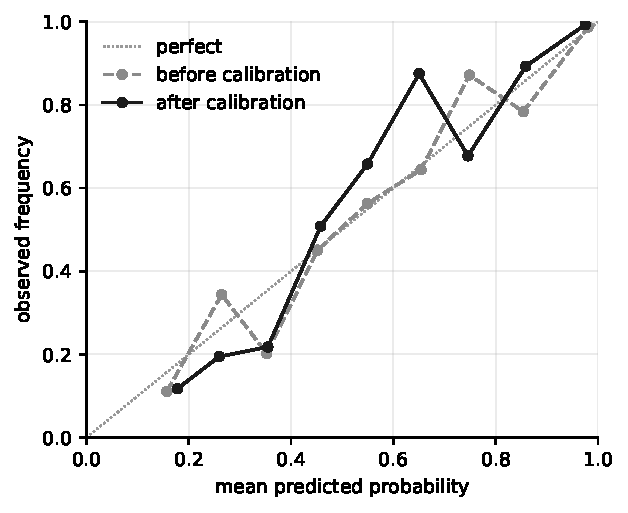
\includegraphics[width=.62\textwidth]{calibration_ngram.pdf}
  \caption[Reliability of the n-gram engine on the development split]{%
  Reliability of the n-gram engine on the development split, before and
  after calibration. Only this engine appears: the rule baseline has no
  probability at all, and the language model's confidence is self reported, so
  neither belongs on an axis of calibrated probability. Generated by
  \code{scripts/make\_report\_figures.py} from
  \rpath{models/dev_metrics.json}.}
  \label{fig:calibration}
\end{figure}

Expected calibration error was \emph{lower before calibration than after it}
(Table~\ref{tab:calibration}, Figure~\ref{fig:calibration}). The uncalibrated
model on this corpus is already close to honest, and refitting a one versus rest
sigmoid per class on a development split of one template per family, then
renormalising, moves classes that were already well behaved.

The calibrator stayed, for two reasons that are both stated rather than assumed.
Macro-F1 is higher with it. And the argument for calibrating at all is about the
number a single finding quotes to a developer, not about an average gap across a
split. What changed is the model card, which now says the error went the wrong
way and by how much. Dropping the calibrator because its summary statistic got
worse, without re-registering, would be tuning on the thing being measured.

One class reached the isotonic switchover, the label covering search boxes and
consent checkboxes. Every other class is calibrated by a sigmoid, and a handful
with no development positives at all are uncalibrated and named as such in the
card.

\section{The third rung, and what it is not}

The third engine is a twelve billion parameter instruction model at four bit
quantization, served locally through a runtime that enforces a JSON response
schema at decode time \cite{ollama-api}. It is optional at runtime, never
required for an audit, and never exercised by continuous integration.

\begin{table}[htbp]
  \centering
  \caption{What each engine says about itself. A run log records this block,
  because a comparison table that named neither the model tag nor the
  quantization would not say what it had measured.}
  \label{tab:engine-describe}
  \begingroup\small\setlength{\tabcolsep}{4pt}
\begin{tabular}{ll}
\toprule
\textbf{Engine property} & \textbf{Value} \\
\midrule
rules confidence kind & \texttt{tier} \\
ngram confidence kind & \texttt{calibrated-probability} \\
ngram execution provider & \texttt{CPUExecutionProvider} \\
ngram ONNX opset & \texttt{26} \\  % results: experiments/results/bench/2026-08-26T20-32-48Z_bench_6457ac7/benchmark.json
llm confidence kind & \texttt{self-reported} \\
llm model tag & \texttt{mistral-nemo:12b-instruct-2407-q4\_K\_M} \\  % results: experiments/results/bench/2026-08-26T20-32-48Z_bench_6457ac7/benchmark.json
llm quantization & \texttt{q4\_K\_M} \\  % results: experiments/results/bench/2026-08-26T20-32-48Z_bench_6457ac7/benchmark.json
llm temperature & \texttt{0.0} \\  % results: experiments/results/bench/2026-08-26T20-32-48Z_bench_6457ac7/benchmark.json
llm batch cap & \texttt{40} \\  % results: experiments/results/bench/2026-08-26T20-32-48Z_bench_6457ac7/benchmark.json
llm structured output & \texttt{json\_schema passed with every request} \\
llm prompt version & \texttt{1.0.0} \\  % results: experiments/results/bench/2026-08-26T20-32-48Z_bench_6457ac7/benchmark.json
\bottomrule
\end{tabular}
\endgroup
\par\smallskip\noindent{\footnotesize Source: \rpath{experiments/results/bench/2026-08-26T20-32-48Z_bench_6457ac7/benchmark.json}}

\end{table}

Three design points decide whether the comparison measures anything at all.

\textbf{The declaration is dropped from what the model sees.} Leaving it in lets
the model read the answer off the page on every clean tier form. The obvious
check, a substring search for the declared token in the serialised payload, is
wrong in both directions: a field named \code{email} that also declares
\code{autocomplete="email"} would trip it, and that combination is common enough
in a clean corpus that the check would have fired on the first real run and been
switched off, while a declaration reaching the payload through a derived value
would not trip it at all. So the property checked is \emph{independence}: pruning
a descriptor and pruning the same descriptor with its declaration stripped must
produce identical payloads. That has neither failure mode and is asserted on
every request rather than reviewed once.

\textbf{The keep list is a floor, not a ceiling.} The specification's list of
what pruning keeps omits several signals the featuriser feeds to the n-gram
model. Withholding a signal one engine has from the other tilts the comparison
exactly as far as handing over the whole document would, in the opposite
direction and with a better conscience. The rule applied is that the language
model sees what the featuriser sees and nothing more.

\textbf{Its threshold block is zero and zero, and that was registered before the
run.} The decision procedure is engine agnostic by confidence value and needs
two numbers, and the specification forbids a self reported confidence from
feeding the threshold policy. The only pair satisfying both is zero and zero.
The two consequences were written down in advance: the language model gets no
threshold protection and accuses on every committed prediction, and the low
confidence finding becomes unreachable for it. Deriving a boundary on the self
reported scale against a precision target, the way the n-gram engine's was
derived, would probably have raised its finding level precision. That it would
have flattered the engine is exactly why it had to be refused before the
measurement rather than after.

\chapter{The audit engine: what gets said out loud}
\label{ch:audit}

A classifier produces a label. An auditor produces an accusation. The distance
between those two is the audit engine, and it is where most of the decisions
that a user actually experiences are made.

\section{The decision procedure}

The procedure is ordered, first match wins, and it runs per control:

\begin{enumerate}
  \item If the control is undetectable, emit \code{UNDETECTABLE\_FIELD} with the
    reason and stop.
  \item If a declaration is present and parses to no token, emit
    \code{AUTOCOMPLETE\_OFF} and stop.
  \item If a declaration is present and is not a specification token, emit
    \code{OFF\_SPEC\_TOKEN} naming the token that was meant, and stop.
  \item If a declaration is present and the classifier is confident it names a
    different field, emit \code{WRONG\_AUTOCOMPLETE} and stop.
  \item If no declaration is present and the classifier is confident, emit
    \code{MISSING\_AUTOCOMPLETE} with the token to add.
  \item Otherwise emit the near miss or structural findings that apply, or
    nothing.
\end{enumerate}

Three places in that ordering had to be read rather than transcribed, and each is
a point where two parts of the specification pull against each other.

\textbf{The composite finding has no branch of its own in the published
pseudocode.} Its trigger reads as \emph{an inferred composite}, which taken
literally fires a warning on every correctly declared month and year input,
while the corpus design makes any finding above the lowest severity on a correct
form a defect. Both hold only if the finding is about the \emph{absence} of the
declaration, so it sits where the missing declaration finding sits and carries
the composite's own fix text.

\textbf{The off switch branch has no stop marker in the pseudocode.} Two other
branches carry one and this one does not, but a declaration of \code{off} parses
to no token, so without the stop a field collects both that finding and the
missing declaration finding: two accusations with two contradictory fixes. The
prose above the pseudocode says first match wins, so it stops.

\textbf{The cross origin frame fix text contradicts the extractor's own
guidance.} The generic template ends by suggesting the control be exposed in
light DOM or the attribute declared on the host, which is sound for a closed
shadow root and nonsense for a frame the page does not own. The more specific
rule wins, and the override is data beside the template rather than a branch
inside a renderer.

\section{Thresholds are per engine, and one of them is a mapping}

\begin{table}[htbp]
  \centering
  \caption{One threshold block per engine. An engine with no block is an error
  rather than an inheritance.}
  \label{tab:thresholds}
  \begingroup\small\setlength{\tabcolsep}{4pt}
\begin{tabular}{lrrr>{\raggedright\arraybackslash}p{.36\textwidth}}
\toprule
\textbf{Engine} & \textbf{tau high} & \textbf{tau low} & \textbf{Target} & \textbf{Basis} \\
\midrule
\texttt{rules} & 0.7000 & 0.4000 & null & rule-tier-band-mapping \\  % results: src/autofill_audit/audit/thresholds.json
\texttt{ngram} & 0.8964 & 0.6278 & 0.9800 & dev split of the seed 20260825 corpus, calibrated n-gram engine \\  % results: src/autofill_audit/audit/thresholds.json
\texttt{llm} & 0.0000 & 0.0000 & null & not a boundary: the self-reported scale decides nothing (spec section 12.1) \\  % results: src/autofill_audit/audit/thresholds.json
\texttt{bert} & 0.8813 & 0.4609 & 0.9800 & dev split of the seed 20260825 corpus, calibrated INT8 encoder. Derived under the identical policy of experiments/predictions/p4-threshold-derivation.md, before the test-split run and before the ship condition of spec section 10.7 was evaluated \\  % results: src/autofill_audit/audit/thresholds.json
\bottomrule
\end{tabular}
\endgroup
\par\smallskip\noindent{\footnotesize Source: \rpath{src/autofill_audit/audit/thresholds.json}}

\end{table}

Table~\ref{tab:thresholds} carries a genuine asymmetry and the report should not
smooth it.

The n-gram engine's boundary is derived on the development split against a
precision target that was committed before the model existed. The rule engine's
is a documented mapping from its six tiers onto the same two bands, and every
key in its block that would hold a measurement is null. That is deliberate. A
regular expression table has no probability, and printing a plausible looking
number in a file the runtime reads would be a law 3 violation with a straight
face. The renderers say in words that a rule tier confidence is a tier and not a
frequency.

The language model's block is zero and zero, for the reason given in
Chapter~\ref{ch:classifiers}: a self reported confidence is forbidden from
gating anything, and the engine still needs two numbers.

\begin{table}[htbp]
  \centering
  \caption{The n-gram engine's derived boundary and what it bought on the
  development split. The precision target was registered before the model
  existed and the derivation script was run unmodified.}
  \label{tab:threshold-derivation}
  \begingroup\small\setlength{\tabcolsep}{4pt}
\begin{tabular}{lr}
\toprule
\textbf{Derived quantity} & \textbf{Value} \\
\midrule
Target precision & 0.9800 \\  % results: src/autofill_audit/audit/thresholds.json
tau high & 0.8964 \\  % results: src/autofill_audit/audit/thresholds.json
tau low & 0.6278 \\  % results: src/autofill_audit/audit/thresholds.json
Dev precision at tau high & 0.9954 \\  % results: src/autofill_audit/audit/thresholds.json
Dev recall at tau high & 0.3701 \\  % results: src/autofill_audit/audit/thresholds.json
Dev accusations & 216 \\  % results: src/autofill_audit/audit/thresholds.json
Dev fields needing an accusation & 581 \\  % results: src/autofill_audit/audit/thresholds.json
\bottomrule
\end{tabular}
\endgroup
\par\smallskip\noindent{\footnotesize Source: \rpath{src/autofill_audit/audit/thresholds.json}}

\end{table}

Two things about Table~\ref{tab:threshold-derivation} need saying rather than
leaving in a file.

\textbf{A precision figure is only as strong as its denominator.} A precision of
one over a handful of accusations and a precision of one over a thousand are the
same number and are not the same claim. The derived block therefore records the
denominators beside the rates, so a reader does not have to go and find out which
it is.

\textbf{A high precision target makes a much quieter tool.} At this boundary the
model raises far fewer accusations than there are fields that need one. That is
what a pre-registered high precision target buys on a model whose calibrated
confidences are honest about how often it is right, and it is the correct outcome
of the policy rather than a failure of it. The policy exists because a false
critical costs a developer far more than a missed one, and this is what
\emph{far more} looks like when it is taken literally.

The two engines' boundaries also had to stay separate. The derived n-gram
boundary sits far above the rule engine's confident band, and a single pair of
thresholds across both would have moved every rule engine finding on every page
as a side effect of training a model. The threshold document therefore carries a
block per engine, the loader takes an engine name, and an engine with no block
raises rather than inheriting one. That was designed to bite when the language
model arrived without a block, and it did, which is how the zero and zero
decision came to be made deliberately and in advance.

\section{The finding catalogue, in brief}

\begin{table}[htbp]
  \centering
  \small
  \begin{tabular}{l>{\raggedright\arraybackslash}p{.66\textwidth}}
    \toprule
    \textbf{Severity} & \textbf{Codes} \\
    \midrule
    critical & \ident{MISSING_AUTOCOMPLETE}, \ident{WRONG_AUTOCOMPLETE},
               \ident{OFF_SPEC_TOKEN} \\
    warning  & \ident{AUTOCOMPLETE_OFF}, \ident{UNLABELED_FIELD},
               \ident{PLACEHOLDER_AS_LABEL}, \ident{SPLIT_FIELD},
               \ident{COMPOSITE_FIELD}, \ident{UNDETECTABLE_FIELD} \\
    info     & \ident{GENERIC_IDENTIFIER}, \ident{WRONG_INPUT_TYPE},
               \ident{MISSING_NAME_ATTR}, \ident{EXTRACTION_INCOMPLETE} \\
    note     & \ident{LOW_CONFIDENCE} \\
    \bottomrule
  \end{tabular}
  \caption{The finding catalogue by severity. Each code carries a trigger, a
  named evidence list, a confidence or a documented tier, and a one line fix.}
  \label{tab:findings-catalogue}
\end{table}

Each carries a trigger, a severity, a named evidence list, a confidence or a
documented tier, and a one line fix as text. There is no mode that edits the
user's markup, because rewriting a production template from a probabilistic
classifier's output is exactly the failure the first law exists to prevent.

\section{A worked example}

The following is real output against a checkout fixture authored in this
repository to get things wrong in the ways real checkouts get them wrong.
Nothing is edited except for trimming the middle of the table.

\begin{shell}
$ autofill-audit audit tests/fixtures/checkout_hostile.html
autofill-audit  file:///.../tests/fixtures/checkout_hostile.html

critical (6)

 control          finding
 .................................................................
 #ck-email        MISSING_AUTOCOMPLETE
                  add autocomplete="email" to #ck-email
                  evidence: declaration:absent, label:email-words
                  [rule tier HIGH]
 #ck-postcode     OFF_SPEC_TOKEN
                  autocomplete="zipcode" is not a valid autofill
                  token; use "postal-code"
                  evidence: declaration:off-spec, label:postcode-words
                  [rule tier HIGH]
 #ck-holder       WRONG_AUTOCOMPLETE
                  #ck-holder declares autocomplete="name" but looks
                  like cc-name; change to autocomplete="cc-name"
                  evidence: declaration:token-mismatch,
                  label:cardholder-words [rule tier HIGH]

warning (8)

 control          finding
 .................................................................
 #input7          PLACEHOLDER_AS_LABEL
                  #input7 uses a placeholder as its label; add a
                  real <label>
                  evidence: structure:placeholder-is-the-only-label
 frame[#hosted-pan] UNDETECTABLE_FIELD
                  the control is inside a cross-origin frame, which
                  is how hosted payment fields are built on purpose;
                  this is not necessarily a defect. Audit that
                  document separately
                  evidence: structure:undetectable

$ echo $?
1
\end{shell}

The before and after that a developer actually applies is one attribute:

\begin{markup}
before, nothing tells the browser what this control is for:

  <input type="text" id="ck-email" placeholder="name@example.com">

after, one attribute, and the browser fills it:

  <input type="email" id="ck-email" autocomplete="email"
         placeholder="name@example.com">
\end{markup}

Three properties of that output are the whole design. Every finding names its
evidence, so it can be argued with. The rule engine's confidence is a tier and
prints as a tier, because turning a regular expression table's output into a
percentage would assert a frequency nobody has measured. And a correct field is
met with silence: the correctly declared card number input on that page does not
appear in the report at all.

\section{The exit code contract}

The process exits non zero when a finding at or above the configured failure
threshold is present, which is what lets the tool drop into a pipeline without a
wrapper script. The threshold is configurable, the default is the critical
severity, and the contract is exercised by end to end tests that run the tool in
a subprocess so that the exit codes are the ones a shell sees rather than the
ones a test harness believes.

\chapter{Method}
\label{ch:method}

\section{What one run is}

An evaluation run takes one split, one engine and one seed, loads every form in
that split through a real browser, extracts descriptors, classifies every keyed
field, runs the audit engine over the same page, and writes five files: a run
log with one row per classified field, a manifest, a metrics document, a
confusion document, and a findings file.

The run log row carries the form identifier, the template, the locale, the tier,
the field selector, the answer key label, the predicted label, the confidence,
the kind of confidence, the runner up, the declared token, the per field
classification latency, and the engine's own name. The manifest carries the
schema version, the commit and whether the tree was dirty, resolved dependency
versions, the corpus manifest digest, the split file digest, the seed, the
engine's self description, the command line, a machine descriptor and the start
and end timestamps.

Three of those deserve a sentence each.

\textbf{The engine field carries the engine's own name.} The specification uses
one label in its run log schema and a different one in its headline table for
the same engine. Carrying two names for one engine across a repository is how a
comparison table becomes ambiguous, so the run log records what the engine calls
itself and a report labels its column however it likes.

\textbf{The confidence kind is mapped rather than copied.} The schema's
vocabulary and the engines' own words are not the same strings, because the
engines' words were made load bearing in the renderers first. The mapping is
written down once and is total: an engine whose word is not in it raises rather
than defaulting to something plausible.

\textbf{The findings file is a fifth artefact the specification does not list.}
Whether a page \emph{needed} an accusation depends on the difference between
declaring nothing, declaring off, and declaring a token outside the
specification, and the run log row carries a declared token that is null in all
three cases. Without the extra file the finding level significance test could not
be reproduced from committed artefacts, and a number nobody can recompute is a
number law 3 does not allow into a report.

\section{Metrics}

Macro-F1 and micro-F1 over the union of observed labels, per slice; per label
precision, recall and F1; a confusion table; abstention rate and accuracy on the
fields the engine did commit to; finding level precision and recall per finding
code; and per field latency percentiles beside the wall clock breakdown.

\textbf{Both averages are always reported.} They disagree here about which of
the two classical engines leads, and a table carrying one of them would be
picking a winner by picking a denominator. The mechanism of the disagreement is
the abstention asymmetry and it is explained where the numbers are, in
Chapter~\ref{ch:headline}.

\textbf{A cell is reported only when it holds enough fields.} Below the
reporting minimum a cell renders the words \emph{insufficient data}, not a
blank, because a blank reads as an oversight and this is a decision. The
threshold is a single constant in the metrics module, imported by everything
that reports, with no per table override, and it was chosen before any corpus
had been generated and before any accuracy had been computed, which is the only
point at which it could be chosen without knowledge of its effect. On this
benchmark it fires on exactly one thing, and what it fires on is itself a
finding: see Section~\ref{sec:accusations}.

\section{The statistical procedure}

The unit of resampling is the template, because fields inside one template share
an author. The test is a paired sign flip permutation at the cluster level,
exhaustive when the arrangement space is small enough to enumerate, with
Benjamini and Hochberg step up correction across the whole comparison family
\cite{benjamini1995}, and a practical effect gate expressed as an absolute
difference in the metric.

\begin{table}[htbp]
  \centering
  \caption{The pre-registered statistical policy and the power the realised
  design has. Every value in the upper half was fixed before the runs.}
  \label{tab:design}
  \begingroup\small\setlength{\tabcolsep}{4pt}
\begin{tabular}{lr}
\toprule
\textbf{Design quantity} & \textbf{Value} \\
\midrule
Resampling unit & \texttt{template\textbackslash\{\}\_id} \\
Clusters in the test split & \texttt{10} \\  % results: experiments/results/analysis/2026-08-26T21-20-11Z_p6-analysis_6457ac7/analysis.json
Sign flip arrangements & \texttt{1024} \\  % results: experiments/results/analysis/2026-08-26T21-20-11Z_p6-analysis_6457ac7/analysis.json
Smallest attainable two sided p & \texttt{0.001953} \\  % results: experiments/results/analysis/2026-08-26T21-20-11Z_p6-analysis_6457ac7/analysis.json
Exhaustive rather than sampled & \texttt{yes} \\
Alpha & \texttt{0.050000} \\  % results: experiments/results/analysis/2026-08-26T21-20-11Z_p6-analysis_6457ac7/analysis.json
False discovery rate & \texttt{0.050000} \\  % results: experiments/results/analysis/2026-08-26T21-20-11Z_p6-analysis_6457ac7/analysis.json
Practical threshold, absolute & \texttt{0.020000} \\  % results: experiments/results/analysis/2026-08-26T21-20-11Z_p6-analysis_6457ac7/analysis.json
Comparison family size & \texttt{33} \\  % results: experiments/results/analysis/2026-08-26T21-20-11Z_p6-analysis_6457ac7/analysis.json
Seed & \texttt{20260825} \\  % results: experiments/results/analysis/2026-08-26T21-20-11Z_p6-analysis_6457ac7/analysis.json
\bottomrule
\end{tabular}
\endgroup
\par\smallskip\noindent{\footnotesize Source: \rpath{experiments/results/analysis/2026-08-26T21-20-11Z_p6-analysis_6457ac7/analysis.json}}

\end{table}

Two decisions in Table~\ref{tab:design} were fixed while fixing them was still
costless, and both would have been contaminated by seeing the numbers.

\textbf{The comparison family is all three engine pairs over the same eleven
comparisons, corrected together.} A three engine benchmark could reasonably have
corrected across one pair, or two, or all three. The temptation is specific and
foreseeable: the comparison this project exists to make is the one against the
language model, and a family containing only that pair would be a third the size
and would produce smaller adjusted p values for exactly the comparisons the
project most wants to be able to report. The size was therefore fixed in the
prediction file, along with the stated consequence that every comparison between
the two classical engines would carry a larger adjusted p than the same
comparison had carried when it was corrected inside a smaller family. It did, and
nobody can report that as a change in the underlying result, because the file
said it would happen.

\textbf{The practical effect gate is absolute.} The external harness's gate is a
relative percentage; this project registered an absolute difference in the
metric. A relative gate turns one pre-registered rule into a different rule in
every slice, because it means something different against a large baseline than
against a small one.

\section{The dependency boundary, and what it cost}

Permutation testing, multiple comparison correction and the verdict vocabulary
are not implemented here. They live in a separate, independently released
evaluation harness \cite{triage} that this project consumes as an ordinary
dependency: not vendored, not submoduled, not copied file by file.

That separation is a deliberate engineering claim. A piece of infrastructure
with exactly one consumer has not been shown to be infrastructure; it has been
shown to be part of that one program. This project is the second consumer, across
a real package boundary, and the friction the boundary exposes is the actual
finding. Vendoring the code would have destroyed that evidence by making the
boundary unobservable.

The friction split cleanly, and the split is more interesting than either
outcome would have been alone.

\textbf{The statistical primitives fit exactly and were used unchanged.} The p
value estimator takes the null distribution as an argument, which is precisely
the seam a caller with its own resampling scheme needs. The correction procedure
needed nothing at all. Its verdict vocabulary already contained the three
categories required plus a fourth for a design whose smallest attainable p value
sits above alpha, which turned out to be the category every comparison in the
first analysis landed in.

\textbf{Everything shaped like a training run did not fit.} The ingestion layer
claims a run log of this shape and then refuses it for having no step field, and
there is no step to add, because the file has no time axis. No public entry point
accepts a cluster assignment. Neither comparison mode is paired, and both reduce
a metric series to a final window mean, which a categorical per field outcome
does not have.

Five issues are filed on that repository, each with a concrete API proposal, and
the ledger in this repository records each one with its status and the
workaround, if any, that stands here in the meantime. Two workarounds exist and
both are labelled in every result file they produce, because a workaround that is
invisible in the output is indistinguishable from a capability: the clustered
null is built here and handed to the harness's estimator, and the practical
effect gate is applied here because the harness's is relative.

The anticipated friction was aimed one layer too low. The ledger predicted,
before the integration began, that categorical outcome support in the permutation
machinery would be the problem. It was not needed at all: the estimator never
sees an outcome, only an effect and a null, both numbers. The categorical part of
the problem lives entirely in the statistic and the statistic is the caller's.
What actually broke was one layer above, in the data model.

One consequence of the boundary is stated here rather than discovered later. The
harness is a development dependency, not a runtime one, because installing it
pulls more than a dozen transitive packages including a training metrics logging
stack, and the audit path never imports it. \textbf{The shipped tool therefore
cannot compute its own significance tests.} The narrower extra that would fix it
is proposed in the ledger.

\section{Reproducibility, and the one artefact that is marked dirty}

One seed reaches the generator, the split assignment, the training script and
any sampling in evaluation, through explicitly passed generator objects. The lock
file is committed and continuous integration installs from it. Every result
directory carries a manifest. Model artefacts are content addressed into every
run that used them. Nothing is ever regenerated to fix a number: if a result is
wrong, a new run is made with a new identifier and the old one stays, because
result files are append only history.

A run produced from a working tree with uncommitted changes is marked dirty in
its manifest and is not citable, and the traceability job fails on a citation of
one. Every evaluation result cited anywhere in this report is marked clean.

\textbf{One artefact is not, and it is the training manifest of the shipped
model.} The model was fitted in the same working session that authored the new
corpus templates, so the tree carried uncommitted changes at the moment of
fitting, and the manifest says so honestly rather than hiding it. What follows
from that is worth being precise about rather than either ignoring or
overstating:

\begin{itemize}
  \item The model artefacts themselves are committed and are content addressed
    into every evaluation run manifest by digest, so \emph{which} model produced
    the headline numbers is not in doubt.
  \item The corpus is content addressed the same way, and its digest in the
    training manifest matches the digest in every evaluation manifest, so the
    model was fitted on the same corpus it was evaluated against.
  \item What is genuinely weaker is the development split evidence: the numbers
    in Tables~\ref{tab:training}, \ref{tab:sweep}, \ref{tab:calibration} and
    \ref{tab:parity} come from a run whose tree state was not pinned to a
    commit. They are reported because they describe how the shipped model was
    built and they should not be silently dropped, and they are flagged here
    because a reader is entitled to know that they sit one notch below the test
    split numbers on the same scale the project applies to everything else.
  \item The fix is procedural rather than technical, it is not applied
    retroactively because that would be a regeneration, and it is listed in
    Chapter~\ref{ch:future}: commit the corpus change first, then train from the
    clean tree.
\end{itemize}

\chapter{The headline experiment}
\label{ch:headline}

\section{The answer, first}

\begin{quote}
Does a fifty kilobyte linear model that runs in microseconds on a CPU get close
enough to a twelve billion parameter model to be the right default for a
developer tool?
\end{quote}

\noindent\textbf{One correction to the question before answering it.} The size in
it is the build specification's own framing, written before the model existed,
and the exported graph is larger than that. The artefact is committed under
\code{models/} and anybody can check its size directly. Nothing in the answer
turns on the figure: the argument is about a linear model that runs on a CPU in
microseconds per field against a twelve billion parameter model on an
accelerator, and that contrast is measured rather than asserted.

\textbf{The premise did not survive the measurement. The linear model did not
have to get close, because it beat the language model on both averages. The rule
table beat both.}

\begin{table}[htbp]
  \centering
  \caption{The headline benchmark: three engines on the test split, both
  averages, and the fourth row that does not exist.}
  \label{tab:headline}
  \begingroup\small\setlength{\tabcolsep}{4pt}
\begin{tabular}{lrrrrrr}
\toprule
\textbf{Engine} & \textbf{Fields} & \textbf{Forms} & \textbf{Templates} & \textbf{Labels} & \textbf{macro-F1} & \textbf{micro-F1} \\  % results: experiments/results/bench/2026-08-26T20-32-48Z_bench_6457ac7/benchmark.json
\midrule
\texttt{rules} & 2317 & 240 & 10 & 36 & 0.7911 & 0.7678 \\  % results: experiments/results/bench/2026-08-26T20-32-48Z_bench_6457ac7/benchmark.json
\texttt{ngram} & 2317 & 240 & 10 & 39 & 0.7394 & 0.8226 \\  % results: experiments/results/bench/2026-08-26T20-32-48Z_bench_6457ac7/benchmark.json
\texttt{llm} & 2317 & 240 & 10 & 38 & 0.6353 & 0.6953 \\  % results: experiments/results/bench/2026-08-26T20-32-48Z_bench_6457ac7/benchmark.json
\midrule
\texttt{bert-onnx-int8} & absent & absent & absent & absent & absent & absent \\  % results: experiments/results/bench/2026-08-26T20-32-48Z_bench_6457ac7/benchmark.json
\bottomrule
\end{tabular}
\endgroup
\par\smallskip\noindent{\footnotesize Source: \rpath{experiments/results/bench/2026-08-26T20-32-48Z_bench_6457ac7/benchmark.json}}

\end{table}

\begin{figure}[htbp]
  \centering
  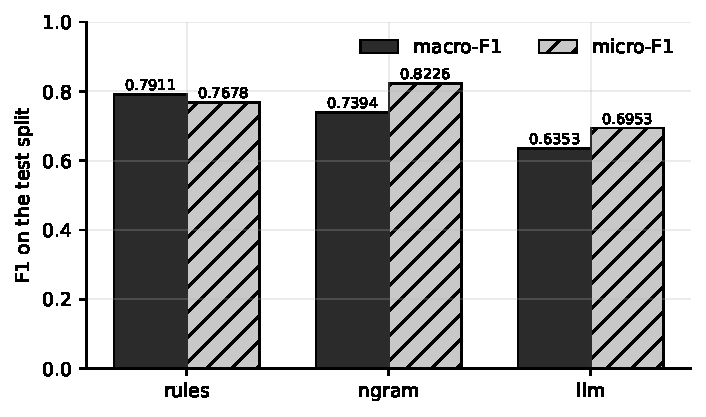
\includegraphics[width=.78\textwidth]{engine_f1.pdf}
  \caption{Both averages for all three engines. They are shown together
  because they disagree about which classical engine leads and agree about which
  came last, and a chart carrying one of them would pick a winner by picking a
  denominator.}
  \label{fig:engine-f1}
\end{figure}

The language model reached \vLlmMacroF{} macro-F1 and \vLlmMicroF{} micro-F1;
the n-gram model \vNgramMacroF{} and \vNgramMicroF{}; the rule table
\vRulesMacroF{} and \vRulesMicroF{}.\footnote{Every number in this paragraph is a
generated macro. The values are in Table~\ref{tab:headline} and the paths they
came from are printed under it.} On this corpus, at this quantization, with this
prompt, the small linear model is not the compromise. It is the better
classifier, and it is also several thousand times faster, needs no accelerator,
and adds nothing meaningful to an install.

The fourth row of Table~\ref{tab:headline} reads \emph{absent} in words rather
than being left blank. A blank cell in a comparison table reads as a measurement
of zero, which would be a fabricated number in the one place a reader trusts
most.

That row is absent for a different reason from the one it originally carried, and
the difference is worth a sentence here rather than only later. The transformer
rung was specified as an optional later phase, and it was then built, fine tuned,
quantized and measured against this same test split. It is the most accurate
classifier this project has produced and it did not ship, because it missed a
latency budget that was fixed before it was trained. This table is the three
engine benchmark it was not part of. Its own run, its result file, and the
arithmetic that rejected it are in Section~\ref{sec:transformer-rung}.

\section{The two averages disagree, and the disagreement is the mechanism}

Macro-F1 says the rule table wins. Micro-F1 says the n-gram model wins. Both are
in the same files and both are correct.

The mechanism is abstention. The rule table answers \code{UNKNOWN} on
\vRulesAbstention{} of the fields and is right on \vRulesCommittedAccuracy{} of
what it does answer. The n-gram model abstains on \vNgramAbstention{} and is
right on \vNgramCommittedAccuracy{}. Abstention costs almost nothing under macro
averaging, where an abstention is a miss on one class, and costs a full share of
the field weighted denominator under micro averaging. A model that answers nearly
everything therefore earns field weighted accuracy and pays label weighted
average every time it guesses a rare class wrongly.

\begin{table}[htbp]
  \centering
  \caption{Abstention, and accuracy on the fields each engine did commit to.}
  \label{tab:abstention}
  \begingroup\small\setlength{\tabcolsep}{4pt}
\begin{tabular}{lrrrr}
\toprule
\textbf{Engine} & \textbf{Fields} & \textbf{Answered UNKNOWN} & \textbf{Abstention rate} & \textbf{Accuracy when committed} \\
\midrule
\texttt{rules} & 2317 & 607 & 0.2620 & 0.9702 \\  % results: experiments/results/bench/2026-08-26T20-32-48Z_bench_6457ac7/benchmark.json
\texttt{ngram} & 2317 & 84 & 0.0363 & 0.8204 \\  % results: experiments/results/bench/2026-08-26T20-32-48Z_bench_6457ac7/benchmark.json
\texttt{llm} & 2317 & 59 & 0.0255 & 0.7037 \\  % results: experiments/results/bench/2026-08-26T20-32-48Z_bench_6457ac7/benchmark.json
\bottomrule
\end{tabular}
\endgroup
\par\smallskip\noindent{\footnotesize Source: \rpath{experiments/results/bench/2026-08-26T20-32-48Z_bench_6457ac7/benchmark.json}}

\end{table}

That is not the rule table being timid. On this corpus abstention is the better
policy, and the rule table has it by construction, because its default branch is
a tier that never clears a threshold.

\section{The language model abstained least of all}

The system prompt tells the model to answer \code{UNKNOWN} when the evidence is
insufficient and not to guess. It abstained on \vLlmAbstention{} of fields, less
than either classical engine, and was right on \vLlmCommittedAccuracy{} of what
it committed to, less than either
(Table~\ref{tab:abstention}).

\textbf{Instructing a model to decline is not equivalent to giving it a
threshold}, and this is the measurement of that gap. It is also the prediction
that failed in the most useful direction: abstention was registered to land
between the two classical engines and landed below both.

\section{Locale and tier}

\begin{table}[htbp]
  \centering
  \caption{Seen locales against the held out locale. The unseen locale column is
  the multilingual claim's actual test: French forms whose templates are also
  unseen.}
  \label{tab:slices}
  \begingroup\small\setlength{\tabcolsep}{4pt}
\begin{tabular}{lrrrr}
\toprule
\textbf{Engine} & \textbf{Seen macro-F1} & \textbf{Seen micro-F1} & \textbf{Unseen macro-F1} & \textbf{Unseen micro-F1} \\  % results: experiments/results/bench/2026-08-26T20-32-48Z_bench_6457ac7/benchmark.json
\midrule
\texttt{rules} & 0.7991 & 0.7743 & 0.7276 & 0.7340 \\  % results: experiments/results/bench/2026-08-26T20-32-48Z_bench_6457ac7/benchmark.json
\texttt{ngram} & 0.7735 & 0.8532 & 0.5637 & 0.6649 \\  % results: experiments/results/bench/2026-08-26T20-32-48Z_bench_6457ac7/benchmark.json
\texttt{llm} & 0.6373 & 0.6981 & 0.6045 & 0.6809 \\  % results: experiments/results/bench/2026-08-26T20-32-48Z_bench_6457ac7/benchmark.json
\bottomrule
\end{tabular}
\endgroup
\par\smallskip\noindent{\footnotesize Source: \rpath{experiments/results/bench/2026-08-26T20-32-48Z_bench_6457ac7/benchmark.json}}

\end{table}

\begin{table}[htbp]
  \centering
  \caption{Macro-F1 by locale.}
  \label{tab:by-locale}
  \begingroup\small\setlength{\tabcolsep}{4pt}
\begin{tabular}{lrrrr}
\toprule
\textbf{Locale} & \textbf{Fields} & \textbf{rules} & \textbf{ngram} & \textbf{llm} \\
\midrule
de-DE & 376 & 0.7259 & 0.7814 & 0.5906 \\  % results: experiments/results/bench/2026-08-26T20-32-48Z_bench_6457ac7/benchmark.json
en-GB & 392 & 0.7904 & 0.8128 & 0.6491 \\  % results: experiments/results/bench/2026-08-26T20-32-48Z_bench_6457ac7/benchmark.json
en-NG & 377 & 0.7998 & 0.8595 & 0.6643 \\  % results: experiments/results/bench/2026-08-26T20-32-48Z_bench_6457ac7/benchmark.json
en-US & 392 & 0.8033 & 0.8024 & 0.6480 \\  % results: experiments/results/bench/2026-08-26T20-32-48Z_bench_6457ac7/benchmark.json
fr-FR & 376 & 0.7276 & 0.5637 & 0.6045 \\  % results: experiments/results/bench/2026-08-26T20-32-48Z_bench_6457ac7/benchmark.json
ja-JP & 404 & 0.8285 & 0.7599 & 0.6345 \\  % results: experiments/results/bench/2026-08-26T20-32-48Z_bench_6457ac7/benchmark.json
\bottomrule
\end{tabular}
\endgroup
\par\smallskip\noindent{\footnotesize Source: \rpath{experiments/results/bench/2026-08-26T20-32-48Z_bench_6457ac7/benchmark.json}}

\end{table}

\begin{figure}[htbp]
  \centering
  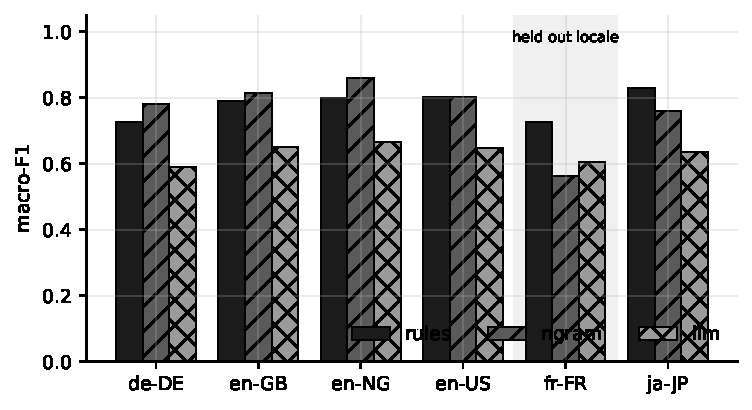
\includegraphics[width=.85\textwidth]{locale_profile.pdf}
  \caption{Macro-F1 by locale, with the held out locale shaded. It is the only
  column in which the language model leads the n-gram model, and it is also a
  column in which the rule table leads them both.}
  \label{fig:locale-profile}
\end{figure}

The held out locale is where broad pretrained world knowledge was supposed to
pay. It is the one slice where the language model leads the n-gram model,
\vLlmUnseenMacroF{} against \vNgramUnseenMacroF{}, and
Chapter~\ref{ch:statistics} shows that this difference does not survive
correction across the family. It is also a slice where the rule table leads both,
at \vRulesUnseenMacroF{}. A vocabulary of localised regular expressions
generalises to an unseen locale better than either learned system does here,
which is an uncomfortable result and is printed as it stands.

\begin{table}[htbp]
  \centering
  \caption{Macro-F1 by markup quality tier.}
  \label{tab:by-tier}
  \begingroup\small\setlength{\tabcolsep}{4pt}
\begin{tabular}{lrrrr}
\toprule
\textbf{Markup tier} & \textbf{Fields} & \textbf{rules} & \textbf{ngram} & \textbf{llm} \\
\midrule
clean & 520 & 0.8677 & 0.9350 & 0.6696 \\  % results: experiments/results/bench/2026-08-26T20-32-48Z_bench_6457ac7/benchmark.json
partial & 519 & 0.8677 & 0.9290 & 0.6522 \\  % results: experiments/results/bench/2026-08-26T20-32-48Z_bench_6457ac7/benchmark.json
mixed & 639 & 0.8005 & 0.7151 & 0.6352 \\  % results: experiments/results/bench/2026-08-26T20-32-48Z_bench_6457ac7/benchmark.json
hostile & 639 & 0.4681 & 0.5409 & 0.5265 \\  % results: experiments/results/bench/2026-08-26T20-32-48Z_bench_6457ac7/benchmark.json
\bottomrule
\end{tabular}
\endgroup
\par\smallskip\noindent{\footnotesize Source: \rpath{experiments/results/bench/2026-08-26T20-32-48Z_bench_6457ac7/benchmark.json}}

\end{table}

\begin{figure}[htbp]
  \centering
  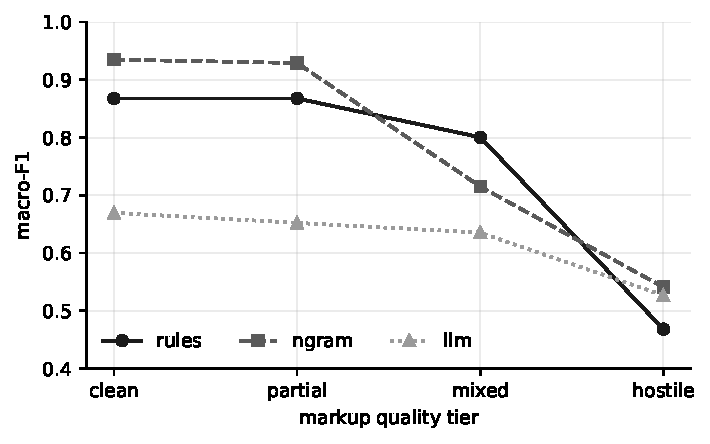
\includegraphics[width=.78\textwidth]{tier_profile.pdf}
  \caption{The tier profile, which is the most informative single picture in the
  benchmark. The two classical engines have strong and opposite slopes; the
  language model is nearly flat and below both until the tiers converge.}
  \label{fig:tier-profile}
\end{figure}

Figure~\ref{fig:tier-profile} is worth reading slowly.

\textbf{The n-gram model is the best engine on clean and partial markup and the
worst classical engine on mixed markup.} It leads on clean at
\vNgramCleanMacroF{} against \vRulesCleanMacroF{}, and trails on mixed at
\vNgramMixedMacroF{} against \vRulesMixedMacroF{}. The mixed tier is the one
built to look like a real page whose sections were written by different teams at
different times. A model that is better on each tier separately and worse on the
tier that mixes them is worth a paragraph rather than a footnote: it suggests the
model is picking up a per page consistency that the mixed tier deliberately
breaks.

\textbf{The hostile tier is where every engine is worst and where the three
converge.} The rule table falls furthest, to \vRulesHostileMacroF{}, because
stripping labels removes most of what a vocabulary of regular expressions has to
work with. The n-gram model reaches \vNgramHostileMacroF{} and the language model
\vLlmHostileMacroF{}. This is the slice where broad pretrained knowledge was
predicted to help most, and none of the differences on it is significant.

The full locale by tier grid, all twenty four cells for all three engines, is
Table~\ref{tab:locale-by-tier} in Appendix~\ref{app:tables}. Every cell clears
the reporting minimum, so nothing in it is suppressed.

\section{What a developer actually experiences}
\label{sec:accusations}

The finding level numbers matter more than the classifier numbers, because they
are what a user of the tool sees. They run through the decision procedure and the
thresholds rather than reporting raw classifier accuracy.

\begin{table}[htbp]
  \centering
  \caption{Finding level precision and recall. Precision is withheld for the two
  classical engines on the second code because neither made enough accusations to
  clear the reporting minimum, and that asymmetry is the finding rather than a
  formatting inconsistency.}
  \label{tab:findings}
  \begingroup\small\setlength{\tabcolsep}{4pt}
\begin{tabular}{llrrrrr}
\toprule
\textbf{Code} & \textbf{Engine} & \textbf{Accusations} & \textbf{Correct} & \textbf{Needed} & \textbf{Precision} & \textbf{Recall} \\
\midrule
\texttt{MISSING\_AUTOCOMPLETE} & \texttt{rules} & 449 & 449 & 790 & 1.0000 & 0.5684 \\  % results: experiments/results/bench/2026-08-26T20-32-48Z_bench_6457ac7/benchmark.json
 & \texttt{ngram} & 334 & 325 & 790 & 0.9731 & 0.4114 \\  % results: experiments/results/bench/2026-08-26T20-32-48Z_bench_6457ac7/benchmark.json
 & \texttt{llm} & 692 & 540 & 790 & 0.7803 & 0.6835 \\  % results: experiments/results/bench/2026-08-26T20-32-48Z_bench_6457ac7/benchmark.json
\midrule
\texttt{WRONG\_AUTOCOMPLETE} & \texttt{rules} & 28 & 28 & 30 & insufficient data & 0.9333 \\  % results: experiments/results/bench/2026-08-26T20-32-48Z_bench_6457ac7/benchmark.json
 & \texttt{ngram} & 23 & 21 & 30 & insufficient data & 0.7000 \\  % results: experiments/results/bench/2026-08-26T20-32-48Z_bench_6457ac7/benchmark.json
 & \texttt{llm} & 125 & 29 & 30 & 0.2320 & 0.9667 \\  % results: experiments/results/bench/2026-08-26T20-32-48Z_bench_6457ac7/benchmark.json
\bottomrule
\end{tabular}
\endgroup
\par\smallskip\noindent{\footnotesize Source: \rpath{experiments/results/bench/2026-08-26T20-32-48Z_bench_6457ac7/benchmark.json}}

\end{table}

\begin{figure}[htbp]
  \centering
  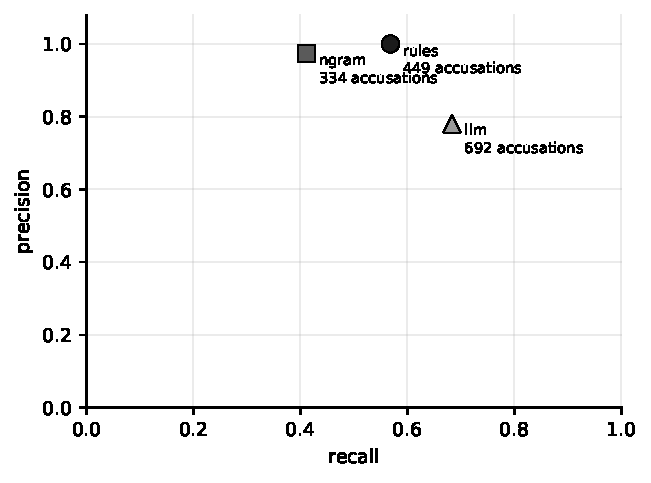
\includegraphics[width=.6\textwidth]{finding_pr.pdf}
  \caption{Where each engine lands on precision against recall for the missing
  declaration finding. \textbf{This compares three threshold policies, not three
  classifiers.} Each engine speaks under its own rule about when to speak, and
  the spread along the horizontal axis is mostly a picture of those rules.}
  \label{fig:finding-pr}
\end{figure}

\textbf{The rule table was right about every field it accused.} It raised
\vRulesMissingAccusations{} missing declaration accusations and
\vRulesMissingWrong{} of them were wrong, at a precision of
\vRulesMissingPrecision{} and a recall of \vRulesMissingRecall{} against
\vMissingNeeded{} fields that needed one.

\textbf{The n-gram model made this project's first wrong accusations.} It raised
\vNgramMissingAccusations{} and was wrong about \vNgramMissingWrong{} of them.
That is the first time in this project that an engine told a developer to add a
token the answer key disagrees with, and it deserves recording rather than
rounding. The threshold policy did not change and the derivation script was run
unmodified; what changed is that the derived boundary now sits on a model whose
development precision at that point was itself below one, so a test split
precision below one is the design working rather than failing. A precision target
is a target, not a guarantee, and a project that reported the target as though it
were the outcome would be reporting a policy as a measurement.

\textbf{The language model found the most real defects and was wrong about
roughly one accusation in five.} It raised \vLlmMissingAccusations{} accusations,
\vLlmMissingWrong{} of them wrong, at a precision of \vLlmMissingPrecision{} and
the highest recall of the three at \vLlmMissingRecall{}. On a developer tool that
means a fifth of the work it hands you is work you should not do.

On the second accusation code the asymmetry is starker.
\vWrongNeeded{} fields needed it, which clears the reporting minimum of
\vReportingMinimum{}, so every recall is reported. Precision is withheld for both
classical engines because neither made enough accusations to be measured, and is
reported for the language model at \vLlmWrongPrecision{} because it made
\vLlmWrongAccusations{}. The engine whose precision can be reported is the one
that accused often enough to be measured, and that is the finding.

None of this is a property of the language model as a classifier. It is a
property of its threshold block, which is zero and zero because a self reported
confidence is forbidden from gating anything, and which was registered before the
run. \textbf{A finding level comparison between these engines is a comparison of
three policies, and that sentence has to travel with the table.}

\section{Latency, and the context that decides whether it matters}

\begin{table}[htbp]
  \centering
  \caption{Per field latency in microseconds, and the share of each run's wall
  clock spent loading and extracting the page.}
  \label{tab:latency}
  \begingroup\small\setlength{\tabcolsep}{4pt}
\begin{tabular}{lrrrr}
\toprule
\textbf{Engine} & \textbf{p50} & \textbf{p95} & \textbf{p99} & \textbf{Load and extract share} \\  % results: experiments/results/bench/2026-08-26T20-32-48Z_bench_6457ac7/benchmark.json
\midrule
\texttt{rules} & 35.2 & 134.0 & 194.7 & 0.9912 \\  % results: experiments/results/bench/2026-08-26T20-32-48Z_bench_6457ac7/benchmark.json
\texttt{ngram} & 165.6 & 261.5 & 355.1 & 0.9874 \\  % results: experiments/results/bench/2026-08-26T20-32-48Z_bench_6457ac7/benchmark.json
\texttt{llm} & 524189.3 & 674727.4 & 774080.6 & 0.0537 \\  % results: experiments/results/bench/2026-08-26T20-32-48Z_bench_6457ac7/benchmark.json
\bottomrule
\end{tabular}
\endgroup
\par\smallskip\noindent{\footnotesize Source: \rpath{experiments/results/bench/2026-08-26T20-32-48Z_bench_6457ac7/benchmark.json}}

\end{table}

\begin{table}[htbp]
  \centering
  \caption{Where each run's wall clock actually went, in seconds.}
  \label{tab:walltime}
  \begingroup\small\setlength{\tabcolsep}{4pt}
\begin{tabular}{lrrrrr}
\toprule
\textbf{Engine} & \textbf{Load} & \textbf{Extract} & \textbf{Classify} & \textbf{Render} & \textbf{Total} \\
\midrule
\texttt{rules} & 131.7 & 4.4 & 0.1 & 0.01 & 137.4 \\  % results: experiments/results/bench/2026-08-26T20-32-48Z_bench_6457ac7/benchmark.json
\texttt{ngram} & 131.8 & 4.4 & 0.5 & 0.02 & 137.9 \\  % results: experiments/results/bench/2026-08-26T20-32-48Z_bench_6457ac7/benchmark.json
\texttt{llm} & 133.0 & 4.9 & 1280.2 & 0.03 & 2565.8 \\  % results: experiments/results/bench/2026-08-26T20-32-48Z_bench_6457ac7/benchmark.json
\bottomrule
\end{tabular}
\endgroup
\par\smallskip\noindent{\footnotesize Source: \rpath{experiments/results/bench/2026-08-26T20-32-48Z_bench_6457ac7/benchmark.json}}

\end{table}

\begin{figure}[htbp]
  \centering
  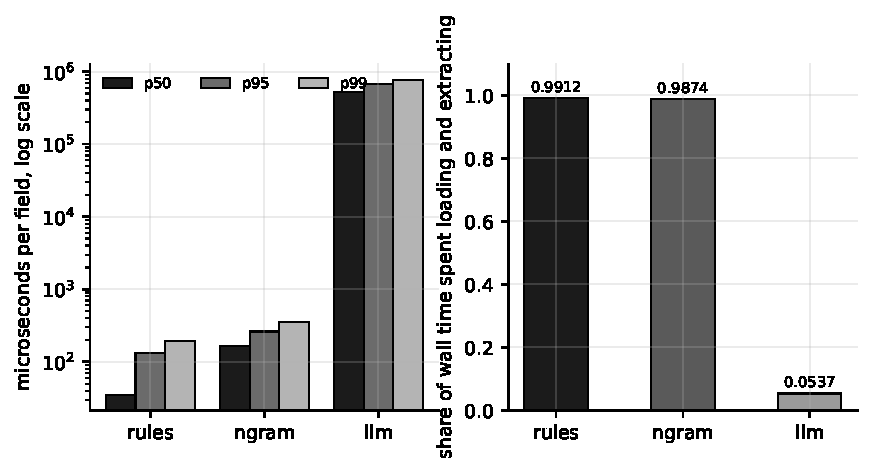
\includegraphics[width=.95\textwidth]{latency.pdf}
  \caption{Latency percentiles on a log axis, beside the share of wall time the
  browser takes. The log axis is not a stylistic choice: a linear one is
  unreadable across this range.}
  \label{fig:latency}
\end{figure}

The two classical engines run on a CPU with the inference session warmed and its
threads pinned, and both are comfortably inside a millisecond per field:
\vRulesLatencyNinetyFive{} and \vNgramLatencyNinetyFive{} microseconds at the
ninety fifth percentile. The language model runs on a warmed local accelerator
and reaches \vLlmLatencyNinetyFive{}, about \vLatencyRatio{} times the rule
table's figure at the same percentile.

\textbf{The language model's figure is a share, not a per call measurement.} It
classifies a whole page in one request, so its per field number is a batch's
elapsed time divided by the fields in that batch. Batching amortises the round
trip, which makes the figure flattering rather than harsh, and it is not
comparable against a per call measurement. The engine's own description says so
and the run manifest records it.

The row that turns a latency difference into a product difference is the share of
wall time. For the rule engine the browser is \vRulesLoadShare{} of the run and
for the n-gram engine \vNgramLoadShare{}, so the classifier is a rounding error
on a page load and celebrating the difference between their latency columns would
be celebrating nothing. For the language model the browser is \vLlmLoadShare{}
and the classifier is the rest. One is a classifier you do not wait for. The
other is one you do.

In wall clock, over the identical page set: about \vRulesMinutes{} minutes for
the rule engine, \vNgramMinutes{} for the n-gram engine, and \vLlmMinutes{} for
the language model.

\textbf{This is the finding that survives contact with real pages.} The accuracy
gap depends on the corpus being synthetic. The runtime inversion does not.

\section{What the language model run did, and what it did not}

\begin{table}[htbp]
  \centering
  \caption{The language model run, including the failure mode that did not
  occur.}
  \label{tab:llm-run}
  \begingroup\small\setlength{\tabcolsep}{4pt}
\begin{tabular}{lr}
\toprule
\textbf{Quantity} & \textbf{Value} \\
\midrule
Requests & 480 \\  % results: experiments/results/bench/2026-08-26T20-32-48Z_bench_6457ac7/benchmark.json
Attempts & 480 \\  % results: experiments/results/bench/2026-08-26T20-32-48Z_bench_6457ac7/benchmark.json
Requests needing a retry & 0 \\  % results: experiments/results/bench/2026-08-26T20-32-48Z_bench_6457ac7/benchmark.json
Requests still failing after the retry & 0 \\  % results: experiments/results/bench/2026-08-26T20-32-48Z_bench_6457ac7/benchmark.json
Fields scored UNKNOWN by a schema failure & 0 \\  % results: experiments/results/bench/2026-08-26T20-32-48Z_bench_6457ac7/benchmark.json
Smallest batch & 3 \\  % results: experiments/results/bench/2026-08-26T20-32-48Z_bench_6457ac7/benchmark.json
Largest batch & 23 \\  % results: experiments/results/bench/2026-08-26T20-32-48Z_bench_6457ac7/benchmark.json
Median batch & 8 \\  % results: experiments/results/bench/2026-08-26T20-32-48Z_bench_6457ac7/benchmark.json
Fields per request cap & 40 \\  % results: experiments/results/bench/2026-08-26T20-32-48Z_bench_6457ac7/benchmark.json
Prompt tokens & 677632 \\  % results: experiments/results/bench/2026-08-26T20-32-48Z_bench_6457ac7/benchmark.json
Completion tokens & 159126 \\  % results: experiments/results/bench/2026-08-26T20-32-48Z_bench_6457ac7/benchmark.json
\midrule
Monetary cost & null \\
\bottomrule
\end{tabular}
\endgroup
\par\smallskip\noindent{\footnotesize Source: \rpath{experiments/results/bench/2026-08-26T20-32-48Z_bench_6457ac7/benchmark.json}}

\end{table}

\textbf{Schema compliance was perfect, and that was not predicted.} Across
\vLlmRequests{} requests, \vLlmRetried{} needed a retry, \vLlmFailed{} still
failed after one, and \vLlmUnresolved{} fields were scored \code{UNKNOWN} by a
schema failure. Passing the response schema with the request and letting the
server constrain decoding appears to remove the failure mode outright. The retry
ladder is still there and is still tested against recorded transcripts including
deliberately malformed ones; on this run it never fired. A benchmark whose most
interesting failure mode did not occur is a result, and the honest report of it is
the zero rather than a paragraph about robustness.

\textbf{Cost is recorded as null rather than zero.} The calls were local. Zero is
a measurement and the electricity was not free; null is the absence of one. No
price list was retrieved, so no list price estimate is computed, and the price
table document in this repository deliberately contains no prices.

\section{The engine order in the benchmark was a methodological choice}

The engines ran with the language model first, which is not the order the tables
present. The two classical engines take a couple of minutes each of browser time
with no inference call in them, so running the language model last would have
meant several idle minutes before its first call, against a bounded keep alive
policy. A keep alive expiry inside a measured run would have put a cold model
load into the per field latency distribution. Warming immediately before and
running it first avoids measuring the disk.

\section{The two classical engines reproduced their previous run exactly}

Every prediction and every finding, field for field across all \vTestFields{}
fields, and every metric identical to the previous measurement on the same
corpus. Only the latency columns differ, because those are re-measured rather
than recomputed.

That was not the purpose of re-running them. It is the strongest reproducibility
evidence this project has produced and it is worth the sentence.

\section{The transformer that led the table and did not ship}
\label{sec:transformer-rung}

A distilled multilingual encoder was fine tuned on the same training split,
exported to ONNX, quantized to eight bit integers with dynamic activations, and
measured against this same test split through the same runner
\cite{onnxruntime-quantization}. It scores \vBertMacroF{} macro-F1 and
\vBertMicroF{} micro-F1, which makes it the most accurate classifier this project
has measured, and it is not an engine the tool offers.

The condition that rejected it was fixed before it existed, in the first commit
of the phase, ahead of the training dependencies being installed. It is a
conjunction of three bars and the verdict is arithmetic rather than editorial.
The unseen locale had to beat the n-gram model's \vNgramUnseenMacroF{} by at
least \vBertUnseenMargin{}, that is reach \vBertBarUnseen{}, and it reached
\vBertUnseenMacroF{}. The whole split had to stay within \vBertOverallTolerance{}
of the n-gram model's \vNgramMacroF{}, that is not fall below \vBertBarOverall{},
and it reached \vBertMacroF{}. The ninety fifth percentile latency per field had
to sit at or under \vBertBarLatency{} microseconds, and it measured
\vBertLatencyNinetyFive{}.

Two of three is a no ship, and the condition says so in as many words
specifically because two of three with a wide margin on the two is the case where
it would be tempting to reconsider. The margins are wide. The engine beat the n
gram model on every locale and on every tier: the held out locale by
\vBertUnseenGain{}, the hostile tier by \vBertHostileGain{}, the whole split by
\vBertOverallGain{}, and the recall of \code{MISSING\_AUTOCOMPLETE} by
\vBertMissingRecallGain{} at a precision of \vBertMissingPrecision{} against the
n-gram model's \vNgramMissingPrecision{}. Corrected across a family of
\vBertFamilySize{} comparisons over \vBertPairs{} engine pairs, the held out
locale, the hostile tier and the recall gain survive and the whole split
difference does not.

It still does not ship, because the third bar is a budget rather than a target,
and a budget that bends when the numbers are good was never a budget. Per field
the engine costs about \vBertLatencyRatio{} times the n-gram model at the same
percentile on the same pinned single thread session. In whole page terms that
turns classification from a fraction of a percent of the run into
\vBertClassifyShare{} of it, with the browser still \vBertLoadShare{}. So the
cost is not that the tool would feel slow. It is that the classifier's share of
the work would grow by a factor of forty in a tool whose own measurements say the
classifier was never the bottleneck, while adding a tokenizer, a second model
format, and a model file of \vBertIntEightMegabytes{} megabytes that this
repository cannot hold.

The parity contract was written in two parts before either export existed,
because demanding exactness from a quantizer is demanding that it not work. The
first part passed: the FP32 graph agreed with the trained model on the argmax of
every one of the \vBertParityRows{} development rows, with a maximum absolute
logit difference of \vBertParityDelta{} against a ceiling of
\vBertParityTolerance{}. The second part did not. Dynamic INT8 was required to
agree with the FP32 graph on at least \vBertIntEightAgreementBar{} of development
rows and to give up at most \vBertIntEightDropBar{} of development macro-F1; it
agreed on \vBertIntEightAgreement{} and gave up \vBertIntEightDrop{}. Both bounds
are missed, neither by much, and both are recorded rather than adjusted. Under
the pre-registered rule that is a second and independent failure of the latency
bar, which is defined on the quantized engine.

What the specification predicted about this rung was that the advantage would be
concentrated in the held out locale and the hostile tier and would be small or
negative on the clean tier, where the n-gram model already has the label text.
The first two held: both gains are larger than the whole split gain, which is
what concentration has to mean to be checkable. The third did not. The clean tier
gained \vBertCleanGain{}, where the phase had predicted less than
\vPracticalThreshold{}. It is a small contradiction and it points somewhere: on a
clean page the encoder is not seeing anything the linear model cannot see, so the
gap that remains is about how the two generalise from a label they have both been
shown.

The result that survives this corpus being synthetic is not the accuracy number.
It is the shape of the trade. A pretrained multilingual encoder buys most of its
advantage exactly where a bag of character n-grams is weakest, on a locale it was
never trained on and on markup stripped of its labels, and it charges two orders
of magnitude of arithmetic for it.

\chapter{Is the difference significant}
\label{ch:statistics}

\section{What was run}

A paired sign flip permutation clustered at the template level, exhaustive over
the full arrangement space, with step up correction across a family of
\vFamilySize{} comparisons, and an absolute practical effect gate. The design
quantities are in Table~\ref{tab:design}.

The test split holds \vTestTemplates{} templates, which gives \vArrangements{}
arrangements and a smallest attainable two sided p value of \vMinAttainableP{},
comfortably below the pre-registered level of \vAlpha{}. \textbf{Every
comparison in this analysis is decidable}, which was not true of the first
measurement this project made and is the whole point of the corpus repair
described in Chapter~\ref{ch:corpus}.

\section{The outcome categories, including the empty ones}

\begin{table}[htbp]
  \centering
  \caption{Every verdict category in the family of comparisons, including the
  two that came back empty. A summary listing only the categories that occurred
  would drop them on exactly the runs where nothing landed in them.}
  \label{tab:outcomes}
  \begingroup\small\setlength{\tabcolsep}{4pt}
\begin{tabular}{lr}
\toprule
\textbf{Verdict} & \textbf{Comparisons} \\
\midrule
improvement & 11 \\  % results: experiments/results/analysis/2026-08-26T21-20-11Z_p6-analysis_6457ac7/analysis.json
regression & 5 \\  % results: experiments/results/analysis/2026-08-26T21-20-11Z_p6-analysis_6457ac7/analysis.json
significant but below the practical threshold & 0 \\  % results: experiments/results/analysis/2026-08-26T21-20-11Z_p6-analysis_6457ac7/analysis.json
no significant change & 17 \\  % results: experiments/results/analysis/2026-08-26T21-20-11Z_p6-analysis_6457ac7/analysis.json
inconclusive: the design cannot reach alpha & 0 \\  % results: experiments/results/analysis/2026-08-26T21-20-11Z_p6-analysis_6457ac7/analysis.json
\midrule
total & 33 \\  % results: experiments/results/analysis/2026-08-26T21-20-11Z_p6-analysis_6457ac7/analysis.json
\bottomrule
\end{tabular}
\endgroup
\par\smallskip\noindent{\footnotesize Source: \rpath{experiments/results/analysis/2026-08-26T21-20-11Z_p6-analysis_6457ac7/analysis.json}}

\end{table}

Table~\ref{tab:outcomes} carries all five categories. Two are worth pointing at
because they are empty.

\textbf{Significant but below the practical threshold: \vBelowThreshold{}.} This
category exists because a difference can be certain and still be too small to
act on, and a reporting scheme that silently merges it into either neighbour is
a reporting scheme that will one day sell a rounding error as a result. On this
family nothing landed in it. It is printed anyway.

\textbf{Inconclusive because the design cannot reach alpha: \vUnderpowered{}.}
This is the category that held all \vOldFamilySize{} comparisons of the first
analysis, when the test split had \vOldClusters{} clusters and a smallest
attainable p of \vOldMinAttainableP{}. It is now empty, which is the measurable
result of the repair.

\section{What is certified, and what is not}

\begin{table}[htbp]
  \centering
  \caption{All comparisons in the family, read in the direction they were
  measured. The full table is Table~\ref{tab:comparisons} in
  Appendix~\ref{app:tables}; this one repeats its shape for reference.}
  \label{tab:cross-check}
  \begingroup\small\setlength{\tabcolsep}{4pt}
\begin{tabular}{lr}
\toprule
\textbf{Cross check} & \textbf{Comparisons} \\
\midrule
Comparisons checked & 33 \\  % results: experiments/results/analysis/2026-08-26T21-20-11Z_p6-analysis_6457ac7/analysis.json
Verdicts that agree & 33 \\  % results: experiments/results/analysis/2026-08-26T21-20-11Z_p6-analysis_6457ac7/analysis.json
Verdicts that disagree & 0 \\  % results: experiments/results/analysis/2026-08-26T21-20-11Z_p6-analysis_6457ac7/analysis.json
\bottomrule
\end{tabular}
\endgroup
\par\smallskip\noindent{\footnotesize Source: \rpath{experiments/results/analysis/2026-08-26T21-20-11Z_p6-analysis_6457ac7/analysis.json}}

\end{table}

\textbf{Certified against the language model, after correction:} the rule table
leads it overall and on the seen locales, and both classical engines lead it on
clean and on partial markup. The language model's missing declaration recall is
certified better than both, and its precision on both accusation codes is
certified worse than both.

\textbf{Not certified:} everything on the hostile tier, everything on the held
out locale, and the language model against the n-gram model overall. Those are
precisely the slices where the language model was expected to do well, and the
honest report of them is that the differences are not large enough to call at
\vClusters{} clusters, in either direction.

\textbf{Not the same statement as no difference.} Comparisons in the \emph{no
significant change} category are comparisons where this design, with this cluster
count, could not resolve the effect. Reading them as evidence of equivalence
would be reading the absence of a certificate as a certificate.

The complete list, every comparison with its effect, its exact p value, its
adjusted p value and its verdict, is Table~\ref{tab:comparisons}.

\section{One reading hazard, stated explicitly}

The comparison names in the result file read \code{baseline\_vs\_candidate} and
the effect is computed as candidate minus baseline. A comparison named for the
language model against the rule table with a verdict of \emph{improvement}
therefore means \textbf{the rule table improved over the language model}, not the
reverse.

The file is self describing: every comparison carries its baseline and its
candidate by name. But the string reads backwards at a glance, which is exactly
the kind of thing that ends up in a report as a sentence pointing the wrong way.
The table generator never renders the comparison name as a sentence. It reads the
baseline, the candidate and the effect and builds the sentence, and the
\emph{Comparison} column of Table~\ref{tab:comparisons} is that sentence.

\section{The family size was fixed in advance, and it cost something}

Every comparison between the two classical engines carries a larger adjusted p
value in this analysis than the same comparison carried when it was corrected
inside the smaller family of the previous phase. The underlying p values did not
move. The earlier analysis file is untouched and is still in the repository.

That was registered before the runs, with the reason: the comparison this phase
existed to make was the one against the language model, and a family containing
only that pair would have been a third the size and would have produced smaller
adjusted p values for exactly the comparisons the project most wanted to be able
to report. Fixing the family size while it was still costless is the only way
that sentence can be written afterwards without it being an excuse.

\section{The harness's own verdicts, as a cross check}

The external harness carries its own end to end verdict machinery. Its
statistical gate and its underpowered gate are the ones used above. Its practical
gate reads a relative percentage where this project pre-registered an absolute
difference, so a disagreement between the two verdict columns would be that gap
and nothing else.

It was run alongside on the same numbers as a visible cross check.
\vCrossCheckChecked{} comparisons were checked and \vCrossCheckDisagreements{}
disagreed. That gap therefore changed no verdict on this data, which is worth
saying plainly and is not a reason to withdraw the filed issue: a gap that happens
not to bite on one dataset is still a gap, and the dataset it would bite on is any
slice with a small baseline.

\section{The secondary analysis, and why nothing cites it}

A secondary analysis clustered by form rather than by template reaches
significance easily. It is computed, it is in the result file, and it is labelled
anticonservative everywhere it appears, because clustering by form asserts that
two locales of one template are independent, which is a stronger claim than this
project's design makes.

Nothing in this report, in the README, or in any document in this repository
cites it as evidence. It is present so that the difference between the two
clusterings is visible rather than assertable, and that is the only reason it is
present.

\chapter{What was predicted, and what was wrong}
\label{ch:predictions}

\section{Why the predictions are here at all}

A prediction committed after the measurement is not a prediction. Every
prediction in this project was written into a file, committed, and a continuous
integration job verifies that the prediction commit is an ancestor of the commit
carrying the result files it predicts about. That check is the only mechanism
that makes the fourth law more than an intention.

The predictions are printed beside the outcomes because that is the only form in
which a prediction is worth anything. A report that showed only the outcomes
would be indistinguishable from a report whose author had decided afterwards
which results were interesting.

\begin{table}[htbp]
  \centering
  \caption{The eight claims registered before the benchmark ran, the number that
  settled each one, and the outcome. The measured column is read from the result
  files by the table generator, so a prediction cannot be scored generously by
  whoever writes the report.}
  \label{tab:predictions}
  \begin{longtable}{p{.34\textwidth}p{.30\textwidth}p{.28\textwidth}}
\toprule
\textbf{Registered before the run} & \textbf{Measured} & \textbf{Outcome} \\
\midrule
\endfirsthead
\toprule
\textbf{Registered before the run} & \textbf{Measured} & \textbf{Outcome} \\
\midrule
\endhead
\bottomrule
\endfoot
The language model beats the n-gram model on the hostile tier & llm 0.5265 against ngram 0.5409 & wrong: it lost \\  % results: experiments/results/bench/2026-08-26T20-32-48Z_bench_6457ac7/benchmark.json experiments/results/test/2026-08-26T20-32-48Z_p6-llm_6457ac7/metrics.json
The language model beats the n-gram model on the held out locale & llm 0.6045 against ngram 0.5637 & held, and not certified after correction \\  % results: experiments/results/bench/2026-08-26T20-32-48Z_bench_6457ac7/benchmark.json experiments/results/test/2026-08-26T20-32-48Z_p6-llm_6457ac7/metrics.json
The language model does not beat the rule table on the held out locale & llm 0.6045 against rules 0.7276 & held \\  % results: experiments/results/bench/2026-08-26T20-32-48Z_bench_6457ac7/benchmark.json experiments/results/test/2026-08-26T20-32-48Z_p6-llm_6457ac7/metrics.json
Latency differs by three orders of magnitude or more & p95 674727.4 against 134.0 & held \\  % results: experiments/results/bench/2026-08-26T20-32-48Z_bench_6457ac7/benchmark.json experiments/results/test/2026-08-26T20-32-48Z_p6-llm_6457ac7/metrics.json
Schema failures above zero and below one request in twenty & 0 retried of 480 requests & wrong: exactly none \\  % results: experiments/results/bench/2026-08-26T20-32-48Z_bench_6457ac7/benchmark.json experiments/results/test/2026-08-26T20-32-48Z_p6-llm_6457ac7/metrics.json
The n-gram model stays the right default & ngram macro-F1 0.7394 against llm 0.6353 & held, for a stronger reason than the one registered \\  % results: experiments/results/bench/2026-08-26T20-32-48Z_bench_6457ac7/benchmark.json experiments/results/test/2026-08-26T20-32-48Z_p6-llm_6457ac7/metrics.json
tel-national read as tel occurs; username read as email does not & tel-national as tel 14; username as email 0 & held in both directions \\  % results: experiments/results/bench/2026-08-26T20-32-48Z_bench_6457ac7/benchmark.json experiments/results/test/2026-08-26T20-32-48Z_p6-llm_6457ac7/metrics.json
Abstention lands between the two classical engines & llm 0.0255, ngram 0.0363, rules 0.2620 & wrong: below both \\  % results: experiments/results/bench/2026-08-26T20-32-48Z_bench_6457ac7/benchmark.json experiments/results/test/2026-08-26T20-32-48Z_p6-llm_6457ac7/metrics.json
\end{longtable}
\par\smallskip\noindent{\footnotesize Source: \rpath{experiments/results/bench/2026-08-26T20-32-48Z_bench_6457ac7/benchmark.json}}
\par\noindent{\footnotesize Source: \rpath{experiments/results/test/2026-08-26T20-32-48Z_p6-llm_6457ac7/metrics.json}}

\end{table}

\section{Four held and four did not}

\textbf{The four that failed are the more interesting half}, and two of them
should be read first.

\textbf{Schema compliance was predicted to fail sometimes, and never failed.}
The registered claim was that the retry rate would be above zero and below one
request in twenty. It was exactly zero across every request of the run. The
mechanism appears to be that passing the response schema with the request lets
the server constrain decoding, which removes the failure mode rather than
reducing it. The retry ladder was built for a problem that, on this serving
route, does not arise. It is still there and still tested, because the next
serving route may not have that property.

\textbf{Abstention went the wrong way.} It was registered to land between the two
classical engines, on the reasoning that a model instructed to decline would
decline more than a model with no such instruction and less than a rule table
whose default branch abstains by construction. It landed below both. Instructing
a model to decline is not equivalent to giving it a threshold, and this is the
measurement of that difference.

\textbf{The hostile tier prediction was wrong in the direction that matters
most.} The hostile tier is where labels are stripped and only obfuscated
identifiers survive, which is where broad pretrained knowledge was supposed to
pay for itself. The language model lost there too.

\textbf{The confusion prediction was wrong in direction as well as in detail.}
The failure was expected to be over claiming: fields that are not personal data
read as though they were. The largest single confusion is the reverse, fields
whose answer key is \code{UNKNOWN} read as the label for a control with no
autofill meaning. The model declines more readily than predicted on the fields
where declining is wrong, while declining less readily overall than either
classical engine. Table~\ref{tab:predicted-pairs} in Appendix~\ref{app:tables}
gives the counts for every confusion pair the specification named in advance, and
Table~\ref{tab:confusions} gives the largest confusions each engine actually
makes.

\section{The pattern across every phase of this project}

Read across all four prediction files rather than only this one, a pattern is
visible and it is not flattering to the intuition that produced the predictions.

\textbf{Every prediction that failed was about a model. Every prediction that
held was about the system.} The predictions that held were the ones where the
mechanism was already understood: page load dominates because a browser is slow;
the n-gram engine is slower per field than the rule table because it enumerates
n-grams in interpreted code; latency differs by orders of magnitude because one
engine is a regular expression match and the other is a forward pass. The ones
that failed were the ones where a mechanism was assumed rather than measured: the
model will generalise better across locales; broad knowledge will help on
degraded markup; instructing a model to abstain will make it abstain.

Two earlier phases are worth listing beside this one, because the pattern is what
makes them worth listing.

At the phase that built the n-gram model, the prediction that the derived
decision threshold would sit \emph{below} the rule engine's confident band was
wrong in the other direction: it sits well above it. That single wrong prediction
is the reason the two engines carry separate threshold blocks, and it is the most
consequential wrong prediction in the project.

At the first evaluation phase, three predictions about the model winning all
failed, and a fourth about which confusion pairs would appear failed completely:
not one of the four pairs named in advance occurred even once, in either
direction, for either engine.

\section{The temptation that was registered against}

The prediction file for this benchmark records, in advance, the specific
temptation that a three engine comparison creates: to correct across the one
engine pair the project cared about rather than across all three. It also records
the consequence of refusing that, which is that every comparison between the two
classical engines would come out with a larger adjusted p than before.

That is the shape a useful pre-registration takes. It is not a forecast of the
result. It is a written commitment to the analysis choices that would otherwise
be made after seeing it.

\chapter{Limitations}
\label{ch:limitations}

The answer in Chapter~\ref{ch:headline} is narrower than it sounds, and the
limits are part of the answer rather than a disclaimer appended to it. They are
in the same document as the result, and the most important ones are repeated in
the same paragraph as the result where they first appear.

\section{What the accuracy result does not license}

\textbf{It does not license any claim that language models are bad at this
task.} What was measured is one twelve billion parameter model at four bit
quantization, with one prompt, no fine tuning, on a synthetic corpus, where the
entire input is a short list of attribute strings.

That input shape is close to the worst case for a system whose advantage is world
knowledge, and close to the best case for one that memorises naming conventions.
A language model asked to reason about a page would have the page. This one had a
pruned descriptor, because giving it the raw document while the n-gram model got
a feature vector would have measured something else entirely.

\textbf{The two classical engines were fitted on this corpus's own training
split. The language model met the corpus for the first time at inference.} That
is a real asymmetry and it points in the direction of the observed result, not
against it. A fine tuned model, a better prompt, a larger model, a higher
precision quantization, or real pages could each move the result, and none of
them was varied.

\textbf{One prompt was tested.} There is no prompt sweep, and there deliberately
is not one, because a prompt sweep chosen after seeing the first result is a
search for a number. Testing several prompts is future work and it requires a
pre-registration of its own.

\section{The corpus is synthetic, and that is the load bearing limitation}

Behaviour on real world pages is unmeasured. Every number in this report is a
measurement on forms this repository generated.

The corpus was designed to be adversarial in the places that matter, and the
markup quality tiers exist precisely so that the easy case does not dominate the
average. But a generated corpus has a generator's habits, and a classifier fitted
on it learns those habits along with the phenomenon. The rule table has the same
exposure in a different form: its vocabulary was written by the same author as
the locale profiles that produce the label text it matches.

That shared authorship is the strongest single reason to distrust the accuracy
gap between the classical engines and the language model, and it is why the
runtime finding is presented as the more robust one.

\section{Six locales is not multilingual}

Six locales, one of them held out. Every locale in the corpus uses either Latin
or Japanese script. There is no right to left locale, no Indic script, no Cyrillic
locale, and no locale whose address grammar differs from the ones present in ways
the generator does not model.

The normalisation layer was hardened against the whole basic multilingual plane
after two property test failures outside the corpus's own alphabet, so the
tokeniser is not the weak point. The locale profiles are, and they are hand
written per locale, which means adding a locale is a real piece of work rather
than a configuration change.

\section{What the tool cannot see}

Repeated here from Chapter~\ref{ch:extractor} because a reader who skipped to the
results should still meet them:

\begin{itemize}
  \item Closed shadow roots are invisible to any script on the page, including
    this one.
  \item Cross origin frames are detected but not read. A hosted payment field is
    a common and correct pattern, and the finding says so rather than implying a
    defect.
  \item Canvas rendered form like widgets are reported as undetectable rather
    than guessed at.
  \item Only the step of a multi step form that is currently in the document is
    audited. There is no click through, because clicking is filling.
  \item \textbf{The tool does not verify that a browser actually autofills.} It
    verifies that the markup gives the browser what it needs. Those are different
    claims and only the second one is made.
\end{itemize}

\section{The evaluation's own limitations}

\textbf{The design resolves large effects, not small ones.} \vClusters{}
clusters give \vArrangements{} arrangements. That is enough to certify the
differences reported as certified in Chapter~\ref{ch:statistics} and not enough
to resolve the ones reported as not certified. More templates per family is the
only thing that helps; more resamples do not, because the test is already
exhaustive.

\textbf{Two statistical components run on this side of the package boundary.}
The clustered null and the absolute practical gate are computed here rather than
in the harness, because the harness has no public entry point for either. Both
are labelled in every result file they produce. The alternative, degrading
silently to unclustered resampling, would have made every comparison look more
significant than it is, and it was the one outcome ruled out before the phase
began.

\textbf{The evaluation runner classifies every form twice.} This is a real defect
and it is documented here rather than in an issue nobody reads. The runner
classifies once directly, which is where the run log's predicted label and per
field latency come from, and once through the audit engine, which is where the
finding codes come from. For the two deterministic engines the passes agree by
construction and cost microseconds. For the language model it doubled the
inference: the run made twice as many requests as there are forms, and about half
its wall clock is the second pass.

Two consequences follow, and the second matters to a reader of
Table~\ref{tab:findings}:

\begin{itemize}
  \item The language model benchmark cost about twice what it needed to.
  \item \textbf{A row's predicted label and its finding codes come from two
    different draws of a model that is not guaranteed to be deterministic.}
    Measured on this run, using the deterministic rule engine as a control for
    the check's own edge cases, the excess disagreement between the two passes is
    on the order of two fields in seven hundred. Small, real, and it should be
    known before anyone builds on the finding level numbers.
\end{itemize}

It is not fixed in this report's phase, and the reason is a rule rather than a
preference: fixing it changes what the evaluation runner does for every engine,
and doing that after seeing the results is the regeneration that this project's
reproducibility rules forbid. The fix is in Chapter~\ref{ch:future} and it is to
pass the first pass's predictions into the audit rather than letting the audit
reclassify, which also turns the two numbers into one fact.

\section{Development split evidence is one notch weaker}

Stated in full in Chapter~\ref{ch:method} and repeated here so that it is met
twice: the training manifest of the shipped model is marked as produced from a
working tree with uncommitted changes. The model artefacts and the corpus are
content addressed into every evaluation manifest, so the identity of what was
measured is not in doubt, but the development split tables in
Chapter~\ref{ch:classifiers} rest on a run whose tree state was not pinned to a
commit. They are reported and they are flagged.

\section{Class imbalance and small denominators}

Several labels in the taxonomy are carried by one template in one position, so
their per label rows in Table~\ref{tab:per-label} rest on small denominators.
Macro-F1 weights every label equally, which means those rows have the same weight
in the headline average as the labels that appear on every form.

That is a deliberate choice rather than an oversight: a label weighted average is
the one that notices when an engine quietly stops predicting a rare class. It
does mean the macro average is noisier than the micro average, and it is another
reason both are reported.

\section{Cost was not measured because nothing was billed}

The monetary cost column is null for every engine. The two classical engines have
no provider and the language model ran locally. Zero is a measurement and the
electricity was not free; null is the absence of one. No vendor price page was
retrieved during this work, so no list price estimate is computed anywhere, and
the price table document in this repository contains no prices on purpose. If a
cost column with a number in it is wanted, that is a retrieval with a date, not a
recollection.

\chapter{Future work}
\label{ch:future}

Ordered by what would change a conclusion in this report, rather than by what
would be pleasant to build.

\section{Measure something real}

\textbf{The single most valuable next measurement is a small, hand labelled set
of real pages.} Every accuracy number in this report is a measurement on a
synthetic corpus, and the strongest objection to all of them is that a generated
corpus has a generator's habits.

This does not require scraping, which is out of scope and stays out of scope.
It requires a small set of pages, labelled by hand against the token set, with
the labelling protocol and the disagreement rate published alongside. A hundred
real forms with a published inter annotator agreement would tell a reader more
about whether the tool works than another thousand generated ones.

The prediction that goes with it should be registered first, and the honest
registration is that the rule table's advantage will shrink, because a
substantial part of it is that its vocabulary and the corpus's label text were
written by the same person.

\section{Fix the double classification in the evaluation runner}

Described in Chapter~\ref{ch:limitations}. The runner classifies each form twice
and the two passes are separate draws for a non deterministic engine, which puts
an excess disagreement on the order of two fields in seven hundred between a
row's predicted label and its finding codes.

The fix is to pass the first pass's predictions into the audit rather than
letting the audit reclassify. It is small, it makes the two numbers one fact, and
it halves the cost of any future language model benchmark. It was not done in the
phase that found it because changing what the runner does for every engine after
seeing the results is exactly the regeneration this project's rules forbid, and
because the honest place for it is a phase that re-registers its predictions and
re-runs everything.

\section{Vary the one thing that was held fixed}

The language model result rests on one model, one quantization and one prompt.
Three variations would each answer a different question, and each needs its own
pre-registration:

\begin{itemize}
  \item \textbf{A higher precision quantization of the same model.} Isolates the
    quantization from the model. Cheap to run and answers an objection that will
    otherwise be raised forever.
  \item \textbf{A second prompt, registered before it is run.} A prompt sweep
    chosen after seeing a result is a search for a number; a second prompt
    registered in advance, with a stated hypothesis about which slice it should
    move, is a measurement.
  \item \textbf{A fine tuned small model.} The comparison as it stands is
    between two engines fitted on the corpus and one that met it at inference.
    Removing that asymmetry is the fairest version of the experiment and it is
    also the most expensive.
\end{itemize}

\section{The transformer rung}

The classifier ladder specifies a small multilingual encoder, fine tuned and
exported with dynamic integer quantization, as an optional fourth engine
\cite{onnxruntime-quantization}. It has not been built, which is why the fourth
row of Table~\ref{tab:headline} reads \emph{absent} in words.

The condition for shipping it is stated in advance and is not negotiable
afterwards: it ships only if it beats a pre-stated metric by a pre-stated margin
within a pre-stated latency budget. If it does not, the deliverable is the
paragraph saying so, with the numbers, and that is a successful outcome rather
than a failed one.

Two things the tier profile in Figure~\ref{fig:tier-profile} suggests it should
be measured against specifically. The mixed tier, where the n-gram model
underperforms its own tier by tier behaviour and where a model with more context
might do better. And the held out locale, where a multilingual encoder's
pretraining is the whole argument for using one.

\section{More templates per family}

The design resolves large effects and not small ones, and the only thing that
improves that is more templates in the test partition. The arithmetic is in
Table~\ref{tab:power-repair}: the relationship between templates and the smallest
attainable p value is steep at the low end and flattens quickly.

The cost is the one already paid once: a regeneration, a retraining, a threshold
rederivation and a re-measurement, with every recorded number moving at once and
an explanation owed in advance.

\section{Close the cross repository tasks}

Five issues are open on the evaluation harness, each with a concrete API
proposal, and two of them block things this project would like to state
plainly:

\begin{itemize}
  \item \textbf{Publication of the harness to a package index.} Until then the
    dependency is a source reference rather than a released version, and the
    project's own rule forbids tagging a stable release while that is true. This
    is the one open task that is a hard blocker rather than an improvement.
  \item \textbf{A narrower dependency set for the harness.} It currently pulls
    more than a dozen transitive packages including a training metrics logging
    stack, which is why it sits in the development extra and why the shipped tool
    cannot compute its own significance tests.
  \item Clustered and paired resampling as a public entry point, an absolute
    practical effect threshold, a stable join key on the verdict output, and a
    typing marker so that values crossing the boundary are checked.
\end{itemize}

\section{Smaller things worth doing}

\begin{itemize}
  \item \textbf{Make the Japanese postal mark reachable.} It is in the rule table
    with a comment saying it cannot fire, because normalisation treats a lone
    symbol as a delimiter. Making it reachable means changing what counts as a
    token character, which churns every golden snapshot and every committed
    fixture expectation, so it is a deliberate change with a cost rather than a
    quiet fix.
  \item \textbf{Ship a model with the wheel, or a documented way to fetch one.}
    A published wheel currently carries no model, so an install runs the rule
    baseline until the user trains one or points the tool at a bundle. The
    behaviour is documented and prints a line rather than failing silently, but
    it means the default install is not the default engine the measurements
    recommend.
  \item \textbf{Widen the hyperparameter grid, with a fresh registration.} The
    sweep chose the edge of its own grid, so the shipped model may be less
    regularised than a wider grid would have chosen. Widening it now would be
    searching for a number; widening it inside a phase that registers first is a
    measurement.
  \item \textbf{Report the reliability curve per class rather than pooled.}
    Calibration made the pooled expected calibration error worse while improving
    macro-F1, and a per class view would say which classes moved and in which
    direction.
\end{itemize}

\section{What is deliberately not future work}

Named so that they stay named and stay out.

Crawling. Form filling. Markup rewriting. Scraping training data. A browser
extension that duplicates the extractor in a second language and doubles the
surface that has to be kept in agreement. Each of those is a boundary rather than
a missing feature, and each is stated as a boundary in the project's own
documentation.

A form filling agent is a genuinely interesting successor and it is named here so
that it stays a separate project rather than becoming a flag on this one.


\appendix
\chapter{The long tables}
\label{app:tables}

The tables in this appendix are the complete versions of grids the chapters
quote from. Every one is generated by \code{scripts/make\_report\_tables.py} from
a committed result file, and the paths are printed under each.

\section{Every comparison in the family}

\begin{center}
\small
\footnotesize
\begin{longtable}{>{\raggedright\arraybackslash}p{.13\textwidth}>{\raggedright\arraybackslash}p{.11\textwidth}>{\raggedright\arraybackslash}p{.15\textwidth}rrr>{\raggedright\arraybackslash}p{.15\textwidth}}
\toprule
\textbf{Comparison} & \textbf{Metric} & \textbf{Slice} & \textbf{Effect} & \textbf{p} & \textbf{adjusted p} & \textbf{Verdict} \\
\midrule
\endfirsthead
\toprule
\textbf{Comparison} & \textbf{Metric} & \textbf{Slice} & \textbf{Effect} & \textbf{p} & \textbf{adjusted p} & \textbf{Verdict} \\
\midrule
\endhead
\bottomrule
\endfoot
rules over llm & \ident{macro_f1} & \ident{all} & 0.1558 & 0.00781 & 0.02578 & improvement \\  % results: experiments/results/analysis/2026-08-26T21-20-11Z_p6-analysis_6457ac7/analysis.json
rules over llm & \ident{macro_f1} & \ident{seen_locales} & 0.1618 & 0.00586 & 0.02578 & improvement \\  % results: experiments/results/analysis/2026-08-26T21-20-11Z_p6-analysis_6457ac7/analysis.json
rules over llm & \ident{macro_f1} & \ident{unseen_locale} & 0.1231 & 0.05664 & 0.08496 & no significant change \\  % results: experiments/results/analysis/2026-08-26T21-20-11Z_p6-analysis_6457ac7/analysis.json
rules over llm & \ident{macro_f1} & \ident{tier:clean} & 0.1981 & 0.01758 & 0.04143 & improvement \\  % results: experiments/results/analysis/2026-08-26T21-20-11Z_p6-analysis_6457ac7/analysis.json
rules over llm & \ident{macro_f1} & \ident{tier:partial} & 0.2155 & 0.01562 & 0.04143 & improvement \\  % results: experiments/results/analysis/2026-08-26T21-20-11Z_p6-analysis_6457ac7/analysis.json
rules over llm & \ident{macro_f1} & \ident{tier:mixed} & 0.1653 & 0.05664 & 0.08496 & no significant change \\  % results: experiments/results/analysis/2026-08-26T21-20-11Z_p6-analysis_6457ac7/analysis.json
rules over llm & \ident{macro_f1} & \ident{tier:hostile} & -0.0584 & 0.19531 & 0.23872 & no significant change \\  % results: experiments/results/analysis/2026-08-26T21-20-11Z_p6-analysis_6457ac7/analysis.json
rules over llm & \ident{finding_precision} & \ident{MISSING_AUTOCOMPLETE} & 0.2197 & 0.00781 & 0.02578 & improvement \\  % results: experiments/results/analysis/2026-08-26T21-20-11Z_p6-analysis_6457ac7/analysis.json
rules over llm & \ident{finding_recall} & \ident{MISSING_AUTOCOMPLETE} & -0.1152 & 0.00195 & 0.02578 & regression \\  % results: experiments/results/analysis/2026-08-26T21-20-11Z_p6-analysis_6457ac7/analysis.json
rules over llm & \ident{finding_precision} & \ident{WRONG_AUTOCOMPLETE} & 0.7680 & 0.00781 & 0.02578 & improvement \\  % results: experiments/results/analysis/2026-08-26T21-20-11Z_p6-analysis_6457ac7/analysis.json
rules over llm & \ident{finding_recall} & \ident{WRONG_AUTOCOMPLETE} & -0.0333 & 1.00000 & 1.00000 & no significant change \\  % results: experiments/results/analysis/2026-08-26T21-20-11Z_p6-analysis_6457ac7/analysis.json
ngram over llm & \ident{macro_f1} & \ident{all} & 0.1041 & 0.08594 & 0.11816 & no significant change \\  % results: experiments/results/analysis/2026-08-26T21-20-11Z_p6-analysis_6457ac7/analysis.json
ngram over llm & \ident{macro_f1} & \ident{seen_locales} & 0.1362 & 0.03516 & 0.06445 & no significant change \\  % results: experiments/results/analysis/2026-08-26T21-20-11Z_p6-analysis_6457ac7/analysis.json
ngram over llm & \ident{macro_f1} & \ident{unseen_locale} & -0.0409 & 0.37500 & 0.41250 & no significant change \\  % results: experiments/results/analysis/2026-08-26T21-20-11Z_p6-analysis_6457ac7/analysis.json
ngram over llm & \ident{macro_f1} & \ident{tier:clean} & 0.2654 & 0.00391 & 0.02578 & improvement \\  % results: experiments/results/analysis/2026-08-26T21-20-11Z_p6-analysis_6457ac7/analysis.json
ngram over llm & \ident{macro_f1} & \ident{tier:partial} & 0.2768 & 0.00391 & 0.02578 & improvement \\  % results: experiments/results/analysis/2026-08-26T21-20-11Z_p6-analysis_6457ac7/analysis.json
ngram over llm & \ident{macro_f1} & \ident{tier:mixed} & 0.0799 & 0.30664 & 0.34894 & no significant change \\  % results: experiments/results/analysis/2026-08-26T21-20-11Z_p6-analysis_6457ac7/analysis.json
ngram over llm & \ident{macro_f1} & \ident{tier:hostile} & 0.0143 & 0.79102 & 0.81573 & no significant change \\  % results: experiments/results/analysis/2026-08-26T21-20-11Z_p6-analysis_6457ac7/analysis.json
ngram over llm & \ident{finding_precision} & \ident{MISSING_AUTOCOMPLETE} & 0.1927 & 0.00781 & 0.02578 & improvement \\  % results: experiments/results/analysis/2026-08-26T21-20-11Z_p6-analysis_6457ac7/analysis.json
ngram over llm & \ident{finding_recall} & \ident{MISSING_AUTOCOMPLETE} & -0.2722 & 0.00195 & 0.02578 & regression \\  % results: experiments/results/analysis/2026-08-26T21-20-11Z_p6-analysis_6457ac7/analysis.json
ngram over llm & \ident{finding_precision} & \ident{WRONG_AUTOCOMPLETE} & 0.6810 & 0.00781 & 0.02578 & improvement \\  % results: experiments/results/analysis/2026-08-26T21-20-11Z_p6-analysis_6457ac7/analysis.json
ngram over llm & \ident{finding_recall} & \ident{WRONG_AUTOCOMPLETE} & -0.2667 & 0.03125 & 0.06066 & no significant change \\  % results: experiments/results/analysis/2026-08-26T21-20-11Z_p6-analysis_6457ac7/analysis.json
ngram over rules & \ident{macro_f1} & \ident{all} & -0.0517 & 0.22656 & 0.26702 & no significant change \\  % results: experiments/results/analysis/2026-08-26T21-20-11Z_p6-analysis_6457ac7/analysis.json
ngram over rules & \ident{macro_f1} & \ident{seen_locales} & -0.0256 & 0.59375 & 0.63206 & no significant change \\  % results: experiments/results/analysis/2026-08-26T21-20-11Z_p6-analysis_6457ac7/analysis.json
ngram over rules & \ident{macro_f1} & \ident{unseen_locale} & -0.1640 & 0.02148 & 0.04727 & regression \\  % results: experiments/results/analysis/2026-08-26T21-20-11Z_p6-analysis_6457ac7/analysis.json
ngram over rules & \ident{macro_f1} & \ident{tier:clean} & 0.0673 & 0.02344 & 0.04834 & improvement \\  % results: experiments/results/analysis/2026-08-26T21-20-11Z_p6-analysis_6457ac7/analysis.json
ngram over rules & \ident{macro_f1} & \ident{tier:partial} & 0.0613 & 0.05469 & 0.08496 & no significant change \\  % results: experiments/results/analysis/2026-08-26T21-20-11Z_p6-analysis_6457ac7/analysis.json
ngram over rules & \ident{macro_f1} & \ident{tier:mixed} & -0.0854 & 0.15820 & 0.20080 & no significant change \\  % results: experiments/results/analysis/2026-08-26T21-20-11Z_p6-analysis_6457ac7/analysis.json
ngram over rules & \ident{macro_f1} & \ident{tier:hostile} & 0.0727 & 0.08203 & 0.11770 & no significant change \\  % results: experiments/results/analysis/2026-08-26T21-20-11Z_p6-analysis_6457ac7/analysis.json
ngram over rules & \ident{finding_precision} & \ident{MISSING_AUTOCOMPLETE} & -0.0269 & 0.01758 & 0.04143 & regression \\  % results: experiments/results/analysis/2026-08-26T21-20-11Z_p6-analysis_6457ac7/analysis.json
ngram over rules & \ident{finding_recall} & \ident{MISSING_AUTOCOMPLETE} & -0.1570 & 0.01758 & 0.04143 & regression \\  % results: experiments/results/analysis/2026-08-26T21-20-11Z_p6-analysis_6457ac7/analysis.json
ngram over rules & \ident{finding_precision} & \ident{WRONG_AUTOCOMPLETE} & -0.0870 & 0.04688 & 0.08141 & no significant change \\  % results: experiments/results/analysis/2026-08-26T21-20-11Z_p6-analysis_6457ac7/analysis.json
ngram over rules & \ident{finding_recall} & \ident{WRONG_AUTOCOMPLETE} & -0.2333 & 0.09375 & 0.12375 & no significant change \\  % results: experiments/results/analysis/2026-08-26T21-20-11Z_p6-analysis_6457ac7/analysis.json
\end{longtable}
\par\smallskip\noindent{\footnotesize Source: \rpath{experiments/results/analysis/2026-08-26T21-20-11Z_p6-analysis_6457ac7/analysis.json}}

\captionof{table}{All comparisons in the corrected family, read in the direction
they were measured. The \emph{Comparison} column is built from the baseline, the
candidate and the effect rather than from the comparison name, which reads
backwards at a glance.}
\label{tab:comparisons}
\end{center}

\section{The locale by tier grid}

\begin{center}
\small
\begin{longtable}{llrrrr}
\toprule
\textbf{Locale} & \textbf{Tier} & \textbf{Fields} & \textbf{rules} & \textbf{ngram} & \textbf{llm} \\
\midrule
\endfirsthead
\toprule
\textbf{Locale} & \textbf{Tier} & \textbf{Fields} & \textbf{rules} & \textbf{ngram} & \textbf{llm} \\
\midrule
\endhead
\bottomrule
\endfoot
de-DE & clean & 84 & 0.7962 & 0.9612 & 0.6732 \\  % results: experiments/results/bench/2026-08-26T20-32-48Z_bench_6457ac7/benchmark.json
de-DE & hostile & 104 & 0.3838 & 0.5401 & 0.4420 \\  % results: experiments/results/bench/2026-08-26T20-32-48Z_bench_6457ac7/benchmark.json
de-DE & mixed & 104 & 0.7518 & 0.7561 & 0.5888 \\  % results: experiments/results/bench/2026-08-26T20-32-48Z_bench_6457ac7/benchmark.json
de-DE & partial & 84 & 0.7962 & 0.9522 & 0.6740 \\  % results: experiments/results/bench/2026-08-26T20-32-48Z_bench_6457ac7/benchmark.json
en-GB & clean & 88 & 0.8741 & 0.9902 & 0.6029 \\  % results: experiments/results/bench/2026-08-26T20-32-48Z_bench_6457ac7/benchmark.json
en-GB & hostile & 108 & 0.4667 & 0.6258 & 0.5611 \\  % results: experiments/results/bench/2026-08-26T20-32-48Z_bench_6457ac7/benchmark.json
en-GB & mixed & 108 & 0.7493 & 0.7829 & 0.6478 \\  % results: experiments/results/bench/2026-08-26T20-32-48Z_bench_6457ac7/benchmark.json
en-GB & partial & 88 & 0.8741 & 0.9902 & 0.6826 \\  % results: experiments/results/bench/2026-08-26T20-32-48Z_bench_6457ac7/benchmark.json
en-NG & clean & 85 & 0.8741 & 0.9902 & 0.7011 \\  % results: experiments/results/bench/2026-08-26T20-32-48Z_bench_6457ac7/benchmark.json
en-NG & hostile & 104 & 0.4453 & 0.6284 & 0.5656 \\  % results: experiments/results/bench/2026-08-26T20-32-48Z_bench_6457ac7/benchmark.json
en-NG & mixed & 104 & 0.7790 & 0.8753 & 0.6555 \\  % results: experiments/results/bench/2026-08-26T20-32-48Z_bench_6457ac7/benchmark.json
en-NG & partial & 84 & 0.8741 & 0.9902 & 0.6791 \\  % results: experiments/results/bench/2026-08-26T20-32-48Z_bench_6457ac7/benchmark.json
en-US & clean & 88 & 0.8741 & 0.9902 & 0.7210 \\  % results: experiments/results/bench/2026-08-26T20-32-48Z_bench_6457ac7/benchmark.json
en-US & hostile & 108 & 0.4667 & 0.5704 & 0.5333 \\  % results: experiments/results/bench/2026-08-26T20-32-48Z_bench_6457ac7/benchmark.json
en-US & mixed & 108 & 0.8068 & 0.7727 & 0.6267 \\  % results: experiments/results/bench/2026-08-26T20-32-48Z_bench_6457ac7/benchmark.json
en-US & partial & 88 & 0.8741 & 0.9902 & 0.6251 \\  % results: experiments/results/bench/2026-08-26T20-32-48Z_bench_6457ac7/benchmark.json
fr-FR & clean & 84 & 0.7962 & 0.6919 & 0.6373 \\  % results: experiments/results/bench/2026-08-26T20-32-48Z_bench_6457ac7/benchmark.json
fr-FR & hostile & 104 & 0.4002 & 0.3347 & 0.4733 \\  % results: experiments/results/bench/2026-08-26T20-32-48Z_bench_6457ac7/benchmark.json
fr-FR & mixed & 104 & 0.7366 & 0.5842 & 0.6330 \\  % results: experiments/results/bench/2026-08-26T20-32-48Z_bench_6457ac7/benchmark.json
fr-FR & partial & 84 & 0.7962 & 0.6919 & 0.5720 \\  % results: experiments/results/bench/2026-08-26T20-32-48Z_bench_6457ac7/benchmark.json
ja-JP & clean & 91 & 0.9074 & 0.9349 & 0.6100 \\  % results: experiments/results/bench/2026-08-26T20-32-48Z_bench_6457ac7/benchmark.json
ja-JP & hostile & 111 & 0.5060 & 0.5125 & 0.4917 \\  % results: experiments/results/bench/2026-08-26T20-32-48Z_bench_6457ac7/benchmark.json
ja-JP & mixed & 111 & 0.7937 & 0.7098 & 0.6259 \\  % results: experiments/results/bench/2026-08-26T20-32-48Z_bench_6457ac7/benchmark.json
ja-JP & partial & 91 & 0.9074 & 0.9016 & 0.6338 \\  % results: experiments/results/bench/2026-08-26T20-32-48Z_bench_6457ac7/benchmark.json
\end{longtable}
\par\smallskip\noindent{\footnotesize Source: \rpath{experiments/results/bench/2026-08-26T20-32-48Z_bench_6457ac7/benchmark.json}}

\captionof{table}{Macro-F1 for every locale and tier cell, all three engines.
Every cell clears the reporting minimum, so nothing here is suppressed.}
\label{tab:locale-by-tier}
\end{center}

\section{Per label behaviour}

\begin{center}
\small
\begin{longtable}{lrrrr}
\toprule
\textbf{Label} & \textbf{Support} & \textbf{rules} & \textbf{ngram} & \textbf{llm} \\
\midrule
\endfirsthead
\toprule
\textbf{Label} & \textbf{Support} & \textbf{rules} & \textbf{ngram} & \textbf{llm} \\
\midrule
\endhead
\bottomrule
\endfoot
\texttt{CC\_EXP\_SPLIT\_MONTH} & 48 & 1.0000 & 1.0000 & 0.6047 \\  % results: experiments/results/test/2026-08-26T21-15-35Z_p6-rules_6457ac7/metrics.json experiments/results/test/2026-08-26T21-17-53Z_p6-ngram_6457ac7/metrics.json experiments/results/test/2026-08-26T20-32-48Z_p6-llm_6457ac7/metrics.json
\texttt{CC\_EXP\_SPLIT\_YEAR} & 48 & 1.0000 & 1.0000 & 0.6842 \\  % results: experiments/results/test/2026-08-26T21-15-35Z_p6-rules_6457ac7/metrics.json experiments/results/test/2026-08-26T21-17-53Z_p6-ngram_6457ac7/metrics.json experiments/results/test/2026-08-26T20-32-48Z_p6-llm_6457ac7/metrics.json
\texttt{COMPOSITE\_UNSPLIT} & 48 & 0.8293 & 0.9565 & 0.0000 \\  % results: experiments/results/test/2026-08-26T21-15-35Z_p6-rules_6457ac7/metrics.json experiments/results/test/2026-08-26T21-17-53Z_p6-ngram_6457ac7/metrics.json experiments/results/test/2026-08-26T20-32-48Z_p6-llm_6457ac7/metrics.json
\texttt{NOT\_AUTOFILLABLE} & 336 & 0.8819 & 0.9587 & 0.7147 \\  % results: experiments/results/test/2026-08-26T21-15-35Z_p6-rules_6457ac7/metrics.json experiments/results/test/2026-08-26T21-17-53Z_p6-ngram_6457ac7/metrics.json experiments/results/test/2026-08-26T20-32-48Z_p6-llm_6457ac7/metrics.json
\texttt{UNKNOWN} & 120 & 0.3301 & 0.7255 & 0.2458 \\  % results: experiments/results/test/2026-08-26T21-15-35Z_p6-rules_6457ac7/metrics.json experiments/results/test/2026-08-26T21-17-53Z_p6-ngram_6457ac7/metrics.json experiments/results/test/2026-08-26T20-32-48Z_p6-llm_6457ac7/metrics.json
\texttt{address-level1} & 64 & 1.0000 & 0.7211 & 0.9375 \\  % results: experiments/results/test/2026-08-26T21-15-35Z_p6-rules_6457ac7/metrics.json experiments/results/test/2026-08-26T21-17-53Z_p6-ngram_6457ac7/metrics.json experiments/results/test/2026-08-26T20-32-48Z_p6-llm_6457ac7/metrics.json
\texttt{address-level2} & 84 & 0.8000 & 0.6900 & 0.8299 \\  % results: experiments/results/test/2026-08-26T21-15-35Z_p6-rules_6457ac7/metrics.json experiments/results/test/2026-08-26T21-17-53Z_p6-ngram_6457ac7/metrics.json experiments/results/test/2026-08-26T20-32-48Z_p6-llm_6457ac7/metrics.json
\texttt{address-line1} & 24 & 0.6286 & 0.6032 & 0.2901 \\  % results: experiments/results/test/2026-08-26T21-15-35Z_p6-rules_6457ac7/metrics.json experiments/results/test/2026-08-26T21-17-53Z_p6-ngram_6457ac7/metrics.json experiments/results/test/2026-08-26T20-32-48Z_p6-llm_6457ac7/metrics.json
\texttt{address-line2} & 24 & 0.9091 & 0.6364 & 0.7407 \\  % results: experiments/results/test/2026-08-26T21-15-35Z_p6-rules_6457ac7/metrics.json experiments/results/test/2026-08-26T21-17-53Z_p6-ngram_6457ac7/metrics.json experiments/results/test/2026-08-26T20-32-48Z_p6-llm_6457ac7/metrics.json
\texttt{address-line3} & 24 & 0.8837 & 0.6842 & 0.7917 \\  % results: experiments/results/test/2026-08-26T21-15-35Z_p6-rules_6457ac7/metrics.json experiments/results/test/2026-08-26T21-17-53Z_p6-ngram_6457ac7/metrics.json experiments/results/test/2026-08-26T20-32-48Z_p6-llm_6457ac7/metrics.json
\texttt{bday} & 24 & 0.8293 & 0.9362 & 0.8293 \\  % results: experiments/results/test/2026-08-26T21-15-35Z_p6-rules_6457ac7/metrics.json experiments/results/test/2026-08-26T21-17-53Z_p6-ngram_6457ac7/metrics.json experiments/results/test/2026-08-26T20-32-48Z_p6-llm_6457ac7/metrics.json
\texttt{cc-csc} & 96 & 0.8000 & 0.8804 & 0.8977 \\  % results: experiments/results/test/2026-08-26T21-15-35Z_p6-rules_6457ac7/metrics.json experiments/results/test/2026-08-26T21-17-53Z_p6-ngram_6457ac7/metrics.json experiments/results/test/2026-08-26T20-32-48Z_p6-llm_6457ac7/metrics.json
\texttt{cc-exp} & 24 & 0.9333 & 0.8837 & 0.5882 \\  % results: experiments/results/test/2026-08-26T21-15-35Z_p6-rules_6457ac7/metrics.json experiments/results/test/2026-08-26T21-17-53Z_p6-ngram_6457ac7/metrics.json experiments/results/test/2026-08-26T20-32-48Z_p6-llm_6457ac7/metrics.json
\texttt{cc-exp-month} & 24 & 1.0000 & 0.8235 & 0.6111 \\  % results: experiments/results/test/2026-08-26T21-15-35Z_p6-rules_6457ac7/metrics.json experiments/results/test/2026-08-26T21-17-53Z_p6-ngram_6457ac7/metrics.json experiments/results/test/2026-08-26T20-32-48Z_p6-llm_6457ac7/metrics.json
\texttt{cc-exp-year} & 24 & 0.7692 & 0.6667 & 0.6111 \\  % results: experiments/results/test/2026-08-26T21-15-35Z_p6-rules_6457ac7/metrics.json experiments/results/test/2026-08-26T21-17-53Z_p6-ngram_6457ac7/metrics.json experiments/results/test/2026-08-26T20-32-48Z_p6-llm_6457ac7/metrics.json
\texttt{cc-name} & 48 & 0.9677 & 0.7547 & 0.8276 \\  % results: experiments/results/test/2026-08-26T21-15-35Z_p6-rules_6457ac7/metrics.json experiments/results/test/2026-08-26T21-17-53Z_p6-ngram_6457ac7/metrics.json experiments/results/test/2026-08-26T20-32-48Z_p6-llm_6457ac7/metrics.json
\texttt{cc-number} & 96 & 0.8075 & 0.8639 & 0.9005 \\  % results: experiments/results/test/2026-08-26T21-15-35Z_p6-rules_6457ac7/metrics.json experiments/results/test/2026-08-26T21-17-53Z_p6-ngram_6457ac7/metrics.json experiments/results/test/2026-08-26T20-32-48Z_p6-llm_6457ac7/metrics.json
\texttt{cc-type} & 72 & 1.0000 & 0.9714 & 0.5743 \\  % results: experiments/results/test/2026-08-26T21-15-35Z_p6-rules_6457ac7/metrics.json experiments/results/test/2026-08-26T21-17-53Z_p6-ngram_6457ac7/metrics.json experiments/results/test/2026-08-26T20-32-48Z_p6-llm_6457ac7/metrics.json
\texttt{country} & 96 & 0.8421 & 0.7630 & 0.3051 \\  % results: experiments/results/test/2026-08-26T21-15-35Z_p6-rules_6457ac7/metrics.json experiments/results/test/2026-08-26T21-17-53Z_p6-ngram_6457ac7/metrics.json experiments/results/test/2026-08-26T20-32-48Z_p6-llm_6457ac7/metrics.json
\texttt{country-name} & 48 & 0.2545 & 0.6250 & 0.4458 \\  % results: experiments/results/test/2026-08-26T21-15-35Z_p6-rules_6457ac7/metrics.json experiments/results/test/2026-08-26T21-17-53Z_p6-ngram_6457ac7/metrics.json experiments/results/test/2026-08-26T20-32-48Z_p6-llm_6457ac7/metrics.json
\texttt{current-password} & 48 & 0.0000 & 0.8889 & 0.6667 \\  % results: experiments/results/test/2026-08-26T21-15-35Z_p6-rules_6457ac7/metrics.json experiments/results/test/2026-08-26T21-17-53Z_p6-ngram_6457ac7/metrics.json experiments/results/test/2026-08-26T20-32-48Z_p6-llm_6457ac7/metrics.json
\texttt{email} & 144 & 0.9565 & 0.9329 & 0.9531 \\  % results: experiments/results/test/2026-08-26T21-15-35Z_p6-rules_6457ac7/metrics.json experiments/results/test/2026-08-26T21-17-53Z_p6-ngram_6457ac7/metrics.json experiments/results/test/2026-08-26T20-32-48Z_p6-llm_6457ac7/metrics.json
\texttt{family-name} & 84 & 0.9091 & 0.7547 & 0.7891 \\  % results: experiments/results/test/2026-08-26T21-15-35Z_p6-rules_6457ac7/metrics.json experiments/results/test/2026-08-26T21-17-53Z_p6-ngram_6457ac7/metrics.json experiments/results/test/2026-08-26T20-32-48Z_p6-llm_6457ac7/metrics.json
\texttt{given-name} & 84 & 0.9091 & 0.7027 & 0.7750 \\  % results: experiments/results/test/2026-08-26T21-15-35Z_p6-rules_6457ac7/metrics.json experiments/results/test/2026-08-26T21-17-53Z_p6-ngram_6457ac7/metrics.json experiments/results/test/2026-08-26T20-32-48Z_p6-llm_6457ac7/metrics.json
\texttt{name} & 24 & 1.0000 & 0.8163 & 0.7164 \\  % results: experiments/results/test/2026-08-26T21-15-35Z_p6-rules_6457ac7/metrics.json experiments/results/test/2026-08-26T21-17-53Z_p6-ngram_6457ac7/metrics.json experiments/results/test/2026-08-26T20-32-48Z_p6-llm_6457ac7/metrics.json
\texttt{new-password} & 96 & 0.7114 & 0.9495 & 0.8108 \\  % results: experiments/results/test/2026-08-26T21-15-35Z_p6-rules_6457ac7/metrics.json experiments/results/test/2026-08-26T21-17-53Z_p6-ngram_6457ac7/metrics.json experiments/results/test/2026-08-26T20-32-48Z_p6-llm_6457ac7/metrics.json
\texttt{one-time-code} & 48 & 0.7692 & 0.6917 & 0.7105 \\  % results: experiments/results/test/2026-08-26T21-15-35Z_p6-rules_6457ac7/metrics.json experiments/results/test/2026-08-26T21-17-53Z_p6-ngram_6457ac7/metrics.json experiments/results/test/2026-08-26T20-32-48Z_p6-llm_6457ac7/metrics.json
\texttt{organization} & 48 & 1.0000 & 0.7273 & 0.7532 \\  % results: experiments/results/test/2026-08-26T21-15-35Z_p6-rules_6457ac7/metrics.json experiments/results/test/2026-08-26T21-17-53Z_p6-ngram_6457ac7/metrics.json experiments/results/test/2026-08-26T20-32-48Z_p6-llm_6457ac7/metrics.json
\texttt{postal-code} & 105 & 0.7861 & 0.8542 & 0.8646 \\  % results: experiments/results/test/2026-08-26T21-15-35Z_p6-rules_6457ac7/metrics.json experiments/results/test/2026-08-26T21-17-53Z_p6-ngram_6457ac7/metrics.json experiments/results/test/2026-08-26T20-32-48Z_p6-llm_6457ac7/metrics.json
\texttt{sex} & 24 & 1.0000 & 0.9020 & 0.5882 \\  % results: experiments/results/test/2026-08-26T21-15-35Z_p6-rules_6457ac7/metrics.json experiments/results/test/2026-08-26T21-17-53Z_p6-ngram_6457ac7/metrics.json experiments/results/test/2026-08-26T20-32-48Z_p6-llm_6457ac7/metrics.json
\texttt{street-address} & 72 & 0.6154 & 0.6142 & 0.3409 \\  % results: experiments/results/test/2026-08-26T21-15-35Z_p6-rules_6457ac7/metrics.json experiments/results/test/2026-08-26T21-17-53Z_p6-ngram_6457ac7/metrics.json experiments/results/test/2026-08-26T20-32-48Z_p6-llm_6457ac7/metrics.json
\texttt{tel} & 24 & 0.6071 & 0.7200 & 0.6102 \\  % results: experiments/results/test/2026-08-26T21-15-35Z_p6-rules_6457ac7/metrics.json experiments/results/test/2026-08-26T21-17-53Z_p6-ngram_6457ac7/metrics.json experiments/results/test/2026-08-26T20-32-48Z_p6-llm_6457ac7/metrics.json
\texttt{tel-country-code} & 24 & 1.0000 & 1.0000 & 0.8000 \\  % results: experiments/results/test/2026-08-26T21-15-35Z_p6-rules_6457ac7/metrics.json experiments/results/test/2026-08-26T21-17-53Z_p6-ngram_6457ac7/metrics.json experiments/results/test/2026-08-26T20-32-48Z_p6-llm_6457ac7/metrics.json
\texttt{tel-national} & 24 & 0.0000 & 0.5862 & 0.5882 \\  % results: experiments/results/test/2026-08-26T21-15-35Z_p6-rules_6457ac7/metrics.json experiments/results/test/2026-08-26T21-17-53Z_p6-ngram_6457ac7/metrics.json experiments/results/test/2026-08-26T20-32-48Z_p6-llm_6457ac7/metrics.json
\texttt{url} & 24 & 0.8571 & 0.8571 & 0.8571 \\  % results: experiments/results/test/2026-08-26T21-15-35Z_p6-rules_6457ac7/metrics.json experiments/results/test/2026-08-26T21-17-53Z_p6-ngram_6457ac7/metrics.json experiments/results/test/2026-08-26T20-32-48Z_p6-llm_6457ac7/metrics.json
\texttt{username} & 72 & 0.8923 & 0.6949 & 0.8872 \\  % results: experiments/results/test/2026-08-26T21-15-35Z_p6-rules_6457ac7/metrics.json experiments/results/test/2026-08-26T21-17-53Z_p6-ngram_6457ac7/metrics.json experiments/results/test/2026-08-26T20-32-48Z_p6-llm_6457ac7/metrics.json
\end{longtable}
\par\noindent{\footnotesize Source: \rpath{experiments/results/test/2026-08-26T21-15-35Z_p6-rules_6457ac7/metrics.json}}
\par\noindent{\footnotesize Source: \rpath{experiments/results/test/2026-08-26T21-17-53Z_p6-ngram_6457ac7/metrics.json}}
\par\noindent{\footnotesize Source: \rpath{experiments/results/test/2026-08-26T20-32-48Z_p6-llm_6457ac7/metrics.json}}

\captionof{table}{F1 per observed label per engine, with the test split support
beside it. Read the rows against the support column: several labels are carried
by one template in one position.}
\label{tab:per-label}
\end{center}

\section{Confusions}

\begin{center}
\small
\begingroup\small\setlength{\tabcolsep}{4pt}
\begin{tabular}{lllr}
\toprule
\textbf{Engine} & \textbf{Answer key} & \textbf{Predicted} & \textbf{Fields} \\
\midrule
\texttt{rules} & \texttt{NOT\_AUTOFILLABLE} & \texttt{UNKNOWN} & 71 \\  % results: experiments/results/test/2026-08-26T21-15-35Z_p6-rules_6457ac7/metrics.json
 & \texttt{current-password} & \texttt{UNKNOWN} & 48 \\  % results: experiments/results/test/2026-08-26T21-15-35Z_p6-rules_6457ac7/metrics.json
 & \texttt{new-password} & \texttt{UNKNOWN} & 43 \\  % results: experiments/results/test/2026-08-26T21-15-35Z_p6-rules_6457ac7/metrics.json
 & \texttt{street-address} & \texttt{UNKNOWN} & 40 \\  % results: experiments/results/test/2026-08-26T21-15-35Z_p6-rules_6457ac7/metrics.json
 & \texttt{postal-code} & \texttt{UNKNOWN} & 37 \\  % results: experiments/results/test/2026-08-26T21-15-35Z_p6-rules_6457ac7/metrics.json
 & \texttt{country-name} & \texttt{country} & 36 \\  % results: experiments/results/test/2026-08-26T21-15-35Z_p6-rules_6457ac7/metrics.json
 & \texttt{cc-csc} & \texttt{UNKNOWN} & 32 \\  % results: experiments/results/test/2026-08-26T21-15-35Z_p6-rules_6457ac7/metrics.json
 & \texttt{cc-number} & \texttt{UNKNOWN} & 31 \\  % results: experiments/results/test/2026-08-26T21-15-35Z_p6-rules_6457ac7/metrics.json
 & \texttt{address-level2} & \texttt{UNKNOWN} & 28 \\  % results: experiments/results/test/2026-08-26T21-15-35Z_p6-rules_6457ac7/metrics.json
 & \texttt{one-time-code} & \texttt{UNKNOWN} & 18 \\  % results: experiments/results/test/2026-08-26T21-15-35Z_p6-rules_6457ac7/metrics.json
\midrule
\texttt{ngram} & \texttt{country} & \texttt{address-level1} & 30 \\  % results: experiments/results/test/2026-08-26T21-17-53Z_p6-ngram_6457ac7/metrics.json
 & \texttt{username} & \texttt{given-name} & 17 \\  % results: experiments/results/test/2026-08-26T21-17-53Z_p6-ngram_6457ac7/metrics.json
 & \texttt{cc-number} & \texttt{cc-name} & 13 \\  % results: experiments/results/test/2026-08-26T21-17-53Z_p6-ngram_6457ac7/metrics.json
 & \texttt{street-address} & \texttt{one-time-code} & 12 \\  % results: experiments/results/test/2026-08-26T21-17-53Z_p6-ngram_6457ac7/metrics.json
 & \texttt{address-level1} & \texttt{country} & 11 \\  % results: experiments/results/test/2026-08-26T21-17-53Z_p6-ngram_6457ac7/metrics.json
 & \texttt{UNKNOWN} & \texttt{one-time-code} & 10 \\  % results: experiments/results/test/2026-08-26T21-17-53Z_p6-ngram_6457ac7/metrics.json
 & \texttt{UNKNOWN} & \texttt{address-line2} & 9 \\  % results: experiments/results/test/2026-08-26T21-17-53Z_p6-ngram_6457ac7/metrics.json
 & \texttt{country-name} & \texttt{address-level2} & 9 \\  % results: experiments/results/test/2026-08-26T21-17-53Z_p6-ngram_6457ac7/metrics.json
 & \texttt{current-password} & \texttt{new-password} & 8 \\  % results: experiments/results/test/2026-08-26T21-17-53Z_p6-ngram_6457ac7/metrics.json
 & \texttt{NOT\_AUTOFILLABLE} & \texttt{email} & 7 \\  % results: experiments/results/test/2026-08-26T21-17-53Z_p6-ngram_6457ac7/metrics.json
\midrule
\texttt{llm} & \texttt{UNKNOWN} & \texttt{NOT\_AUTOFILLABLE} & 91 \\  % results: experiments/results/test/2026-08-26T20-32-48Z_p6-llm_6457ac7/metrics.json
 & \texttt{country} & \texttt{country-name} & 76 \\  % results: experiments/results/test/2026-08-26T20-32-48Z_p6-llm_6457ac7/metrics.json
 & \texttt{cc-type} & \texttt{NOT\_AUTOFILLABLE} & 43 \\  % results: experiments/results/test/2026-08-26T20-32-48Z_p6-llm_6457ac7/metrics.json
 & \texttt{street-address} & \texttt{address-line1} & 40 \\  % results: experiments/results/test/2026-08-26T20-32-48Z_p6-llm_6457ac7/metrics.json
 & \texttt{COMPOSITE\_UNSPLIT} & \texttt{address-line1} & 36 \\  % results: experiments/results/test/2026-08-26T20-32-48Z_p6-llm_6457ac7/metrics.json
 & \texttt{CC\_EXP\_SPLIT\_MONTH} & \texttt{cc-exp-month} & 22 \\  % results: experiments/results/test/2026-08-26T20-32-48Z_p6-llm_6457ac7/metrics.json
 & \texttt{CC\_EXP\_SPLIT\_YEAR} & \texttt{cc-exp-year} & 22 \\  % results: experiments/results/test/2026-08-26T20-32-48Z_p6-llm_6457ac7/metrics.json
 & \texttt{new-password} & \texttt{current-password} & 20 \\  % results: experiments/results/test/2026-08-26T20-32-48Z_p6-llm_6457ac7/metrics.json
 & \texttt{one-time-code} & \texttt{NOT\_AUTOFILLABLE} & 15 \\  % results: experiments/results/test/2026-08-26T20-32-48Z_p6-llm_6457ac7/metrics.json
 & \texttt{current-password} & \texttt{new-password} & 14 \\  % results: experiments/results/test/2026-08-26T20-32-48Z_p6-llm_6457ac7/metrics.json
\bottomrule
\end{tabular}
\endgroup
\par\noindent{\footnotesize Source: \rpath{experiments/results/test/2026-08-26T21-15-35Z_p6-rules_6457ac7/metrics.json}}
\par\noindent{\footnotesize Source: \rpath{experiments/results/test/2026-08-26T21-17-53Z_p6-ngram_6457ac7/metrics.json}}
\par\noindent{\footnotesize Source: \rpath{experiments/results/test/2026-08-26T20-32-48Z_p6-llm_6457ac7/metrics.json}}

\captionof{table}{The largest confusions each engine makes on the test split.}
\label{tab:confusions}
\end{center}

\begin{center}
\small
\begingroup\small\setlength{\tabcolsep}{4pt}
\begin{tabular}{lrrr}
\toprule
\textbf{Named pair} & \textbf{rules} & \textbf{ngram} & \textbf{llm} \\
\midrule
\texttt{address-level1 as address-level2} & 0 & 0 & 0 \\  % results: experiments/results/test/2026-08-26T21-15-35Z_p6-rules_6457ac7/metrics.json experiments/results/test/2026-08-26T21-17-53Z_p6-ngram_6457ac7/metrics.json experiments/results/test/2026-08-26T20-32-48Z_p6-llm_6457ac7/metrics.json
\texttt{address-level2 as address-level1} & 0 & 0 & 2 \\  % results: experiments/results/test/2026-08-26T21-15-35Z_p6-rules_6457ac7/metrics.json experiments/results/test/2026-08-26T21-17-53Z_p6-ngram_6457ac7/metrics.json experiments/results/test/2026-08-26T20-32-48Z_p6-llm_6457ac7/metrics.json
\texttt{cc-exp as cc-exp-month} & 0 & 1 & 4 \\  % results: experiments/results/test/2026-08-26T21-15-35Z_p6-rules_6457ac7/metrics.json experiments/results/test/2026-08-26T21-17-53Z_p6-ngram_6457ac7/metrics.json experiments/results/test/2026-08-26T20-32-48Z_p6-llm_6457ac7/metrics.json
\texttt{cc-exp-month as cc-exp} & 0 & 0 & 0 \\  % results: experiments/results/test/2026-08-26T21-15-35Z_p6-rules_6457ac7/metrics.json experiments/results/test/2026-08-26T21-17-53Z_p6-ngram_6457ac7/metrics.json experiments/results/test/2026-08-26T20-32-48Z_p6-llm_6457ac7/metrics.json
\texttt{email as username} & 0 & 0 & 0 \\  % results: experiments/results/test/2026-08-26T21-15-35Z_p6-rules_6457ac7/metrics.json experiments/results/test/2026-08-26T21-17-53Z_p6-ngram_6457ac7/metrics.json experiments/results/test/2026-08-26T20-32-48Z_p6-llm_6457ac7/metrics.json
\texttt{tel as tel-national} & 0 & 6 & 0 \\  % results: experiments/results/test/2026-08-26T21-15-35Z_p6-rules_6457ac7/metrics.json experiments/results/test/2026-08-26T21-17-53Z_p6-ngram_6457ac7/metrics.json experiments/results/test/2026-08-26T20-32-48Z_p6-llm_6457ac7/metrics.json
\texttt{tel-national as tel} & 15 & 7 & 14 \\  % results: experiments/results/test/2026-08-26T21-15-35Z_p6-rules_6457ac7/metrics.json experiments/results/test/2026-08-26T21-17-53Z_p6-ngram_6457ac7/metrics.json experiments/results/test/2026-08-26T20-32-48Z_p6-llm_6457ac7/metrics.json
\texttt{username as email} & 0 & 0 & 0 \\  % results: experiments/results/test/2026-08-26T21-15-35Z_p6-rules_6457ac7/metrics.json experiments/results/test/2026-08-26T21-17-53Z_p6-ngram_6457ac7/metrics.json experiments/results/test/2026-08-26T20-32-48Z_p6-llm_6457ac7/metrics.json
\bottomrule
\end{tabular}
\endgroup
\par\smallskip\noindent{\footnotesize Source: \rpath{experiments/results/test/2026-08-26T21-15-35Z_p6-rules_6457ac7/metrics.json}}

\captionof{table}{The confusion pairs named in the specification before any
measurement existed, and how often each actually occurred. Most of them never
did, in either direction, for any engine.}
\label{tab:predicted-pairs}
\end{center}

\section{Form family}

\begin{center}
\small
\begingroup\small\setlength{\tabcolsep}{4pt}
\begin{tabular}{lrrrr}
\toprule
\textbf{Form family} & \textbf{Fields} & \textbf{rules} & \textbf{ngram} & \textbf{llm} \\
\midrule
address & 352 & 0.7222 & 0.4194 & 0.5371 \\  % results: experiments/results/test/2026-08-26T21-15-35Z_p6-rules_6457ac7/metrics.json experiments/results/test/2026-08-26T21-17-53Z_p6-ngram_6457ac7/metrics.json experiments/results/test/2026-08-26T20-32-48Z_p6-llm_6457ac7/metrics.json
checkout & 821 & 0.8414 & 0.6447 & 0.4741 \\  % results: experiments/results/test/2026-08-26T21-15-35Z_p6-rules_6457ac7/metrics.json experiments/results/test/2026-08-26T21-17-53Z_p6-ngram_6457ac7/metrics.json experiments/results/test/2026-08-26T20-32-48Z_p6-llm_6457ac7/metrics.json
login & 216 & 0.6843 & 0.4700 & 0.4476 \\  % results: experiments/results/test/2026-08-26T21-15-35Z_p6-rules_6457ac7/metrics.json experiments/results/test/2026-08-26T21-17-53Z_p6-ngram_6457ac7/metrics.json experiments/results/test/2026-08-26T20-32-48Z_p6-llm_6457ac7/metrics.json
payment & 384 & 0.8570 & 0.5464 & 0.6913 \\  % results: experiments/results/test/2026-08-26T21-15-35Z_p6-rules_6457ac7/metrics.json experiments/results/test/2026-08-26T21-17-53Z_p6-ngram_6457ac7/metrics.json experiments/results/test/2026-08-26T20-32-48Z_p6-llm_6457ac7/metrics.json
signup & 544 & 0.7634 & 0.5521 & 0.5251 \\  % results: experiments/results/test/2026-08-26T21-15-35Z_p6-rules_6457ac7/metrics.json experiments/results/test/2026-08-26T21-17-53Z_p6-ngram_6457ac7/metrics.json experiments/results/test/2026-08-26T20-32-48Z_p6-llm_6457ac7/metrics.json
\bottomrule
\end{tabular}
\endgroup
\par\noindent{\footnotesize Source: \rpath{experiments/results/test/2026-08-26T21-15-35Z_p6-rules_6457ac7/metrics.json}}
\par\noindent{\footnotesize Source: \rpath{experiments/results/test/2026-08-26T21-17-53Z_p6-ngram_6457ac7/metrics.json}}
\par\noindent{\footnotesize Source: \rpath{experiments/results/test/2026-08-26T20-32-48Z_p6-llm_6457ac7/metrics.json}}

\captionof{table}{Macro-F1 by form family.}
\label{tab:by-family}
\end{center}

\section{Label coverage in the corpus}

\begin{center}
\small
\begin{longtable}{lr}
\toprule
\textbf{Label} & \textbf{Keyed fields in the corpus} \\
\midrule
\endfirsthead
\toprule
\textbf{Label} & \textbf{Keyed fields in the corpus} \\
\midrule
\endhead
\bottomrule
\endfoot
\texttt{CC\_EXP\_SPLIT\_MONTH} & 120 \\  % results: corpus/manifest.json
\texttt{CC\_EXP\_SPLIT\_YEAR} & 120 \\  % results: corpus/manifest.json
\texttt{COMPOSITE\_UNSPLIT} & 264 \\  % results: corpus/manifest.json
\texttt{NOT\_AUTOFILLABLE} & 1296 \\  % results: corpus/manifest.json
\texttt{UNKNOWN} & 480 \\  % results: corpus/manifest.json
\texttt{additional-name} & 96 \\  % results: corpus/manifest.json
\texttt{address-level1} & 288 \\  % results: corpus/manifest.json
\texttt{address-level2} & 404 \\  % results: corpus/manifest.json
\texttt{address-line1} & 264 \\  % results: corpus/manifest.json
\texttt{address-line2} & 264 \\  % results: corpus/manifest.json
\texttt{address-line3} & 96 \\  % results: corpus/manifest.json
\texttt{bday} & 96 \\  % results: corpus/manifest.json
\texttt{cc-csc} & 384 \\  % results: corpus/manifest.json
\texttt{cc-exp} & 72 \\  % results: corpus/manifest.json
\texttt{cc-exp-month} & 96 \\  % results: corpus/manifest.json
\texttt{cc-exp-year} & 96 \\  % results: corpus/manifest.json
\texttt{cc-name} & 264 \\  % results: corpus/manifest.json
\texttt{cc-number} & 384 \\  % results: corpus/manifest.json
\texttt{cc-type} & 168 \\  % results: corpus/manifest.json
\texttt{country} & 360 \\  % results: corpus/manifest.json
\texttt{country-name} & 192 \\  % results: corpus/manifest.json
\texttt{current-password} & 168 \\  % results: corpus/manifest.json
\texttt{email} & 600 \\  % results: corpus/manifest.json
\texttt{family-name} & 392 \\  % results: corpus/manifest.json
\texttt{given-name} & 392 \\  % results: corpus/manifest.json
\texttt{honorific-prefix} & 144 \\  % results: corpus/manifest.json
\texttt{honorific-suffix} & 144 \\  % results: corpus/manifest.json
\texttt{name} & 144 \\  % results: corpus/manifest.json
\texttt{new-password} & 360 \\  % results: corpus/manifest.json
\texttt{nickname} & 144 \\  % results: corpus/manifest.json
\texttt{one-time-code} & 240 \\  % results: corpus/manifest.json
\texttt{organization} & 192 \\  % results: corpus/manifest.json
\texttt{postal-code} & 403 \\  % results: corpus/manifest.json
\texttt{sex} & 96 \\  % results: corpus/manifest.json
\texttt{street-address} & 168 \\  % results: corpus/manifest.json
\texttt{tel} & 144 \\  % results: corpus/manifest.json
\texttt{tel-country-code} & 144 \\  % results: corpus/manifest.json
\texttt{tel-extension} & 96 \\  % results: corpus/manifest.json
\texttt{tel-national} & 144 \\  % results: corpus/manifest.json
\texttt{transaction-amount} & 120 \\  % results: corpus/manifest.json
\texttt{url} & 120 \\  % results: corpus/manifest.json
\texttt{username} & 192 \\  % results: corpus/manifest.json
\end{longtable}
\par\smallskip\noindent{\footnotesize Source: \rpath{corpus/manifest.json}}

\captionof{table}{Keyed fields per label across the whole generated corpus. This
is the evidence for the growth rule's clause that every label must be emitted by
at least one answer key, and it is also the honest picture of how uneven the
class distribution is.}
\label{tab:label-coverage}
\end{center}

\chapter{Provenance}
\label{app:provenance}

\section{Every result file this report cites}

Law 3 says that no number appears in this report unless it is reproducible from
a committed file under \code{experiments/results/} whose manifest names a commit
this repository can produce. Table~\ref{tab:provenance} is that chain, written
out.

\begin{center}
\small
\footnotesize
\begin{longtable}{p{.46\textwidth}p{.24\textwidth}ll}
\toprule
\textbf{Run directory} & \textbf{Engine} & \textbf{Commit} & \textbf{Clean} \\
\midrule
\endfirsthead
\toprule
\textbf{Run directory} & \textbf{Engine} & \textbf{Commit} & \textbf{Clean} \\
\midrule
\endhead
\bottomrule
\endfoot
\rpath{experiments/results/test/2026-08-26T21-15-35Z_p6-rules_6457ac7} & \texttt{rules} & \texttt{6457ac7} & yes \\  % results: experiments/results/test/2026-08-26T21-15-35Z_p6-rules_6457ac7
\rpath{experiments/results/test/2026-08-26T21-17-53Z_p6-ngram_6457ac7} & \texttt{ngram} & \texttt{6457ac7} & yes \\  % results: experiments/results/test/2026-08-26T21-17-53Z_p6-ngram_6457ac7
\rpath{experiments/results/test/2026-08-26T20-32-48Z_p6-llm_6457ac7} & \texttt{llm} & \texttt{6457ac7} & yes \\  % results: experiments/results/test/2026-08-26T20-32-48Z_p6-llm_6457ac7
\rpath{experiments/results/analysis/2026-08-26T21-20-11Z_p6-analysis_6457ac7} & \texttt{llm against rules against ngram} & \texttt{6457ac7} & yes \\  % results: experiments/results/analysis/2026-08-26T21-20-11Z_p6-analysis_6457ac7
\rpath{experiments/results/bench/2026-08-26T20-32-48Z_bench_6457ac7} & \texttt{llm against rules against ngram} & \texttt{6457ac7} & yes \\  % results: experiments/results/bench/2026-08-26T20-32-48Z_bench_6457ac7
\rpath{experiments/results/analysis/2026-08-26T02-53-59Z_analysis_336175f} & \texttt{rules against ngram} & \texttt{336175f} & yes \\  % results: experiments/results/analysis/2026-08-26T02-53-59Z_analysis_336175f
\rpath{experiments/results/analysis/2026-08-26T06-23-41Z_p5r-analysis_0d900ff} & \texttt{rules against ngram} & \texttt{0d900ff} & yes \\  % results: experiments/results/analysis/2026-08-26T06-23-41Z_p5r-analysis_0d900ff
\rpath{experiments/results/test/2026-08-26T02-50-54Z_rules_57d2aed} & \texttt{rules} & \texttt{57d2aed} & yes \\  % results: experiments/results/test/2026-08-26T02-50-54Z_rules_57d2aed
\rpath{experiments/results/test/2026-08-26T02-52-08Z_ngram_57d2aed} & \texttt{ngram} & \texttt{57d2aed} & yes \\  % results: experiments/results/test/2026-08-26T02-52-08Z_ngram_57d2aed
\rpath{experiments/results/test/2026-08-26T06-18-34Z_p5r-rules_0d900ff} & \texttt{rules} & \texttt{0d900ff} & yes \\  % results: experiments/results/test/2026-08-26T06-18-34Z_p5r-rules_0d900ff
\rpath{experiments/results/test/2026-08-26T06-21-03Z_p5r-ngram_0d900ff} & \texttt{ngram} & \texttt{0d900ff} & yes \\  % results: experiments/results/test/2026-08-26T06-21-03Z_p5r-ngram_0d900ff
\end{longtable}

\captionof{table}{Every run cited in this report, its engine, the commit its
manifest names, and whether the working tree was clean when it was produced. A
run marked dirty is not citable and the traceability job fails on a citation of
one.}
\label{tab:provenance}
\end{center}

The check is not a pattern match on the shape of a citation. It walks the whole
chain for every reference in every prose file and every LaTeX source: the path
must exist, a manifest must sit beside it or above it, that manifest must name a
commit this repository can produce an object for, and the manifest must not mark
the run dirty.

That distinction was learned the hard way. The job went red on a check that had
passed locally minutes earlier, because the clone had been made at the default
depth of one, so it held only the tip commit and every citation of a run taken in
an earlier commit failed with a message saying the commit does not resolve in
this repository. That sentence was true of the clone and false of the repository.
The failure was reproduced locally before anything was changed, because a
failure that is fixed without being reproduced is a failure that is guessed at.

\section{The result files that are here and are not cited}

Two earlier sets of test split runs are in this repository and nothing in this
report cites them.

The first pair was taken on a corpus whose test partition held one template per
family. Those results were correctly taken and are correctly reported as the
first, underpowered measurement. They are not edited, not moved and not deleted,
because result files are append only history and the honest description of them
is what they are rather than something to be tidied away.

The second pair was taken after the corpus repair and before the language model
existed. Chapter~\ref{ch:corpus} cites those two for exactly one purpose, which
is to show what the repair did to each engine, and
Table~\ref{tab:engines-moved} is that comparison with the caveat attached that
the two columns are not two measurements of the same thing.

\section{Version strings in the committed run logs}

A reader looking at the older run logs will find a tool version string that does
not match the release the results are associated with. That is consistent rather
than wrong: those runs were taken before the version bump, the engine
description records the version that was actually running, and the manifest's
commit resolves to a tree in which that string is correct.

Re-running them to make the string prettier is exactly the regeneration this
project forbids, so they stay, and this paragraph is the explanation.

\section{How to reproduce any number in this report}

\begin{enumerate}
  \item Clone the repository at the commit a manifest names.
  \item Regenerate the corpus from the seed recorded in the corpus manifest and
    the base year recorded beside it. The output is byte identical or the
    generator has a defect.
  \item Install from the committed lock file.
  \item Run the evaluation for the engine and split named in the manifest's
    command line, which is recorded verbatim.
  \item Compare the metrics document against the committed one.
\end{enumerate}

The language model engine is the one step that will not reproduce bit for bit,
and that is recorded rather than papered over: the serving runtime does not
guarantee determinism, temperature and seed are pinned and are recorded in the
run, and the engine description says in words that determinism is not claimed.


% Every entry in refs.bib was actually retrieved and read, and docs/references.md
% carries the retrieval date and the observed status for each. They are all
% listed here rather than only the ones a sentence happens to cite, because the
% bibliography is the reading list of the project rather than a footnote index.
\nocite{*}
\bibliographystyle{plain}
\bibliography{refs}

\end{document}
